\documentclass[11pt]{book}

\usepackage{fullpage}
\usepackage{graphicx}
\usepackage{cite}
\usepackage{times}
\usepackage{setspace}
\usepackage{fancyhdr}
\usepackage{ifthen}
\usepackage[section]{placeins}
\usepackage{booktabs}
\usepackage{graphicx}
\usepackage{pgfplots}
\usepackage{pgfplotstable}
\pgfplotsset{compat=newest}

\setcounter{topnumber}{2}
\setcounter{bottomnumber}{3}
\setcounter{totalnumber}{4}  
\renewcommand{\topfraction}{0.5}
\renewcommand{\bottomfraction}{0.95}
\renewcommand{\textfraction}{0.1}
\renewcommand{\floatpagefraction}{0.7}

\setlength{\abovecaptionskip}{3pt}
\setlength{\belowcaptionskip}{3pt}

\pagestyle{fancy}
\setboolean{@twoside}{false} 
\setlength{\headsep}{25pt}
\setlength{\headheight}{14pt}

% Bar chart color definitions
\definecolor{bblue}{HTML}{4F81BD}
\definecolor{rred}{HTML}{C0504D}

\newcommand{\benchbar}[6] {%
\begin{tikzpicture}
    \begin{axis}[
        width  = 0.5*\textwidth,
        height = 8cm,
        major x tick style = transparent,
        ybar=2*\pgflinewidth,
        bar width=14pt,
        ymajorgrids = true,
        ylabel = {Run time (s)},
        xlabel = {No. of Nodes},
        symbolic x coords={2,4,8},
        xtick = data,
        scaled y ticks = false,
        enlarge x limits=0.25,
        ymin=0,
        legend cell align=left,
        legend style={
                at={(1,1.05)},
                anchor=south east,
                column sep=1ex
        }
    ]
        \addplot[style={rred,fill=rred,mark=none}]
            coordinates {(2,#1) (4,#2) (8,#3)};
        \addplot[style={bblue,fill=bblue,mark=none}]
            coordinates {(2,#4) (4,#5) (8,#6)};
        \legend{Random,Profile Guided}
    \end{axis}
\end{tikzpicture}
}

\begin{document}

\thispagestyle{empty}

\doublespacing

\vspace*{0.5in}

\begin{center}
\LARGE{\textbf{Profile Driven Partitioning Of Parallel Simulation Models}}

\vspace*{0.4in}

  {\large A thesis submitted to the\\[0.20in]
    Division of Research and Advanced Studies\\
    of the University of Cincinnati\\[0.20in]
    in partial fulfillment of the\\
    requirements for the degree of\\[0.20in]
    {\bf MASTER OF SCIENCE}\\[0.20in]
    in the School of Electric and Computing Systems\\
    of the College of Engineering and Applied Sciences\\[0.20in]
    May 23, 2014\\[0.20in]
    by\\[0.20in]
    {\bf AJ Alt}\\
    BS Computer Engineering, University of Cincinnati, 2012\\}
  \vspace{0.5in}
  {\large Thesis Advisor and Committee Chair:  Dr. Philip A. Wilsey}
\end{center}

\clearpage

\setcounter{page}{1}
\pagenumbering{roman}
\clearpage

\chapter*{Abstract} 

A considerable amount of research into effective parallelization for discrete event driven simulation has been conducted over the past few decades. However, most of this research has targeted the parallel simulation infrastructure; focusing on data structures, algorithms, and synchronization methods for the parallel and distributed simulation kernels. While this focus has successfully improved and refined the performance of parallel discrete event simulation kernels, little effort has been directed toward analyzing and preparing the simulation model itself for parallel execution. Model specific optimizations could have significant performance implications, but have been largely ignored. This fact is complicated by the lack of a widely used simulation and modeling language for many domains. The lack of a common language is, however, not entirely insurmountable. For example, the partitioning and assignment of objects from the simulation model onto the hardware platform is generally performed by the simulation infrastructure. While partitioning can have dramatic impacts on the communication frequencies between the concurrently executed objects, most existing parallel simulation infrastructures do little to address this opportunity.

This thesis addresses the partitioning and assignment of objects within a simulation model for parallel execution. The specific target of this effort is to develop a partitioning and assignment strategy for use in the \textsc{warped} parallel simulation kernel that has been developed and maintained at the University of Cincinnati. The focus of the work is to develop a general purpose solution that can function for any simulation model that has been prepared for execution on the \textsc{warped} kernel. The specific solution exploits a sequential kernel from the \textsc{warped} project to pre-simulate the simulation model to obtain profile data regarding the frequency of events communicated between objects. This event frequency data is then used to develop partitions to minimize the amount of event exchanges between the objects in the different partitions. This partition information is then used during the initialization sequences of the \textsc{warped} kernel to assign each partition to a unique processing node in the parallel cluster. This method is independent of the simulation model and compute platform. Experimental results with existing simulation models from the \textsc{warped} project show that this method can achieve up to a six-fold improvement in run time over the naive partitioning algorithm that was previously used by the \textsc{warped} kernel.

\tableofcontents \markright{ }
\listoffigures \markright{ }
\listoftables \markright{ }

\clearpage
\pagenumbering{arabic} \setcounter{page}{1}

\chapter{Introduction}\label{intro} 

The potential performance improvement of distributing a fine-grained computation over a cluster of parallel compute nodes is frequently dominated by the network latency. The time required to send a single message between computers on a local network can be on the order of milliseconds \cite{larson-07}, while modern processors can execute an instruction in much less than a nanosecond \cite{sprangle-02}. Therefore, the run time of a computation that requires frequent communication can be dominated by the costs of sending network messages. Discrete Event Simulation (DES) is one such fine grained computation.

Discrete-event driven simulation (DES) is a widely used mechanism to facilitate modeling of complex physical systems that defy study with standard mathematical methods \cite{law-00}. Unfortunately the desire to model and evaluate increasingly large and complex systems has made executing DES models with conventional sequential simulation engines unacceptably slow. This has lead to an interest in using parallelism to accelerate the performance of DES simulations \cite{fujimoto-90}. Parallel discrete-event simulation (PDES) maps a conventional DES onto a parallel hardware processing platform. In general, these processing platforms are either tightly-coupled shared memory systems or distributed memory Beowulf clusters \cite{hennessy-12}.

Mapping DES onto Beowulf clusters is made difficult due to the fine-grained computation required for processing an event and the frequencies with which new events are created and processed by the PDES engine. For most DES models, the processing requirements for a single event are low, and so the simulation run time can be dominated by message passing costs. In a sequential DES, communicating event information between objects requires, at most, a memory copy. In PDES, sending an event may require that event data be serialized into a network message, communicated, and deserialized at the receiving node. For certain simulation models (\emph{workloads}), this means that much of the simulation time is spent sending network messages. This is especially true when the simulation model is distributed across the parallel compute nodes without regard to the number of messages that will have to be exchanged by the concurrent objects of the parallel simulation. Ultimately the number of exchanged messages will be heavily dependent on each particular simulation model and thus, some form of model specific analysis activity must be performed to determine a suitable partitioning for the simulation model across the parallel compute hardware.

This thesis presents a method of reducing simulation network traffic in PDES simulations while balancing processor load by using profile data to implement a model specific partitioning and assignment capability. The profile based approach uses a small sequential simulator that pre-simulates the model to capture information on how frequently objects within the simulation model exchange event information. This event ``profile data'' is then used to establish a set of partitions that attempt to minimize the amount of event information that will have to be exchanged between objects of different partitions. The identified partitions are then used by the parallel simulation kernel to assign partitions (and the simulation objects therein) to the compute nodes of the parallel Cluster. The effectiveness of this method is demonstrated by implementing profile guided partitioning in the \textsc{warped} PDES kernel. A number of real world models are used to evaluate the effectiveness of the approach against the naive partitioning algorithm currently used by the \textsc{warped} kernel. These studies show that a significant speedups can be achieved when the studied profile based partitioning method is applied to these models.

\section{Principle Hypothesis}

The principle hypothesis of this thesis is that \emph{the overhead of sending events between nodes in a PDES simulation has a large impact on its runtime, and that profile guided partitioning can significantly reduce the amount of events sent between nodes, thereby improving simulation performance}. This thesis explores the event passing characteristics and performance of a number of real world models run in a Time Warp simulator.

\section{Thesis Overview}

The remainder of this thesis is organized as follows:

Chapter \ref{background} gives an explanation of Discrete Event Simulations and the Time Warp protocol for Parallel Discrete Event Simulations. It introduces the concepts of partitioning and load balancing in the context of Parallel Discrete Event Simulations, and gives an overview of the \textsc{warped} Simulation Kernel used in this thesis.

Chapter \ref{relatedWork} reviews some of the related work in the field of partitioning for Parallel Discrete Event Simulation.

Chapter \ref{overview} provides a general explanation of the approach taken in this thesis to performing profiling and Profile Guided Partitioning in Parallel Discrete Event Simulations.

Chapter \ref{implementationDetails} describes the implementation details of the Profile Guided Partitioning used in this thesis and incorporated into the \textsc{warped} simulation kernel.

Chapter \ref{analysis} describes the simulation models and platforms used to evaluate the effectiveness of Profile Guided Partitioning in Time Warp simulations. The Profile Guided Partitioning is compared to the naive partitioning algorithm that was used prior to this thesis.

Finally, Chapter \ref{conclusion} summarizes the thesis and discusses possibilities for future that can be built on the work presented in this thesis.

\chapter{Background}\label{background}

This chapter introduces the concepts central to this thesis. Information on general Discrete Event Simulation (DES) is presented. Next, a description of the general principles of on Parallel Discrete Event Simulation (PDES) is provided. Finally information on the Time Warp distributed synchronization mechanism for PDES and the \textsc{warped} simulation kernel that implements this mechanism is provided.

\section{Discrete Event Simulation}

A Discrete Event Simulation is composed of a set of \emph{simulation object}s. Each simulation object may have a collection of state that changes in response to \emph{events}. Events are messages sent between objects, and can contain data provided by the object that created them. Each event also carries a timestamp that defines when the event should be executed. Events with lower timestamps occur earlier in the simulation than events with higher timestamps. An object may generate 0, 1, or multiple output events in response to an input event \cite{law-00}.

For example, in the case of a digital circuit model, the objects are the gates, and the events are logic signals sent between connected gates. The simulation is not concerned with the physical propagation of the electrical signals across wires. When the output of a gate changes, the simulator calculates the propagation time of the signal, then adds the event to a priority queue that is sorted on the timestamp of events. This queue is often referred to as a Least Time Stamp First queue, or LTSF queue. The simulator then pops an event off of the LTSF queue and advances its simulation clock to the timestamp of that event. The simulator then sends the event to its target object, which calculates its new output and sends events to any connected object. This process repeats until there are no more event exists to be processed, or until a preset simulation time has been reached.

\section{Parallel Discrete Event Simulation}

It is often desirable to attempt to increase performance of a sequential Discrete Event Simulation by distributing the workload across multiple processes (often called \emph{nodes}) that can execute in parallel \cite{fujimoto-90}. In a Parallel Discrete Event Simulation (PDES), the set of simulation objects is partitioned into disjoint subsets. Each partition of objects is assigned to its own \emph{Logical Process} (LP) that executes concurrently. All LPs are able to execute concurrently, processing events destined for the objects they contain.

The parallel approach to DES brings with it a number of challenges. As with any concurrent computation, synchronization is an issue. Because each LP runs at a different speed, it is possible that the simulation times of the LPs will diverge. When this happens, an event with a larger timestamp may be executed before an event with a lower, violating causality of the simulation. There are two main synchronization approaches to preventing causality violations in PDES: \emph{Conservative Synchronization} \cite{bryant-79,chandy-81} and \emph{Optimistic Synchronization} \cite{fujimoto-90,jefferson-85}.

Conservative Synchronization avoids the possibility of causality errors by synchronizing all LPs such that an event is not processed by any LP until all events that may affect it have been processed. If an LP has no events that can be processed safely without potentially violating causality, the process blocks until it is safe to process the event. This is straight forward, but blocking processes wastes processing time, and may lead to deadlocks if a cycle of LPs are waiting on each other in a way that prevents any of them from proceeding. Additionally, since no LP will process an event that might violate causality, the entire simulation can only proceed as quickly as the slowest LP, which is referred to as the \emph{critical path}.

Optimistic Synchronization takes a very different approach, in that it does not attempt to prevent causality violations. Instead, causality errors are detected and the simulation is repaired to a causally consistent state. Time Warp \cite{jefferson-85} is one of the most well-known architectures for Optimistic Synchronization of PDES. In a Time Warp simulator, each LP copies that state of its objects at regular intervals called \emph{checkpoints}, and runs at full speed, as if it will never receive an event that would cause a causality error. If an LP detects that a causality violation has occurred (\emph{i.e.}, it receives an event with a timestamp lower than an event it has already processed), it rolls back the state of its internal objects to a checkpoint before the timestamp of the received event. If the LP performing the rollback had sent to other LPs any events that need to be rolled back, it will send messages (termed \emph{Anti-Messages}) that inform the LPs of the invalid events. This allows all LPs in the simulation to run at full speed, which in turn allows for the possibility that the simulation can run faster than the critical path.

Each LP in a Time Warp synchronized PDES has its own Local Virtual Time (LVT). This is the lowest timestamp of any unprocessed local event. The Global Virtual Time (GVT) is lowest timestamp of any unprocessed event in the entire simulation. Because no events with a timestamp lower than the GVT will ever by processed, it is safe for the simulator to free memory used by events or saved states with lower timestamps \cite{fujimoto-90}.

\section{Partitioning and Load Balancing}

In a Time Warp simulation, even though rollbacks do not impact the performance of the critical path, they are still a large inefficiency as a result of lost processing time \cite{chetlur-06}. An LP that advances its LVT much faster than other LPs will spend most of its time rolling back its state instead of performing useful work. To achieve maximum performance, it is desirable to minimize the number of rollbacks that occur during simulation. Balancing the workload between LPs can help reduce rollbacks by reducing the amount by which any single LP will be able to advance ahead of the others. If all the objects in a simulation require roughly the same amount of time to process a single event, load balancing can be achieved by assigning the same number of simulation objects to each partition.

Even if processing load is balanced between LPs, the partitioning strategy can still have a large impact on the performance of a simulation. Because LPs maintain local causality by executing events in ascending timestamp order, an event sent between two objects on the same partition will never cause a rollback. Therefore, assigning objects that communicate frequently to the same partition can reduce the number of rollbacks, and consequently increase performance.

Another reason that partitioning can have a large impact on performance is that the cost of sending an event is drastically different depending on whether the target of an event is located on the same partition as the source. An intra-partition event will only require that the event data be copied with a single process. However, if an event crosses partition boundaries, it will need to be sent between LPs. If both LPs are located on the same machine on a cluster or on a shared-memory platform, Inter-Process Communication (IPC) will be necessary, which is expensive. If the LPs are located on different nodes on a cluster, a network message will need to be sent, which is even slower than IPC.

Since only cross-partition events can trigger rollbacks, and are slow even if no rollback occurs, partitioning can have a large impact on performance. A naive partitioning algorithm that balances the number of simulation objects between partitions without regard to event characteristics can perform very poorly on real-world models. Consider a model consists of \(k\) separate partitions. If the simulation objects are randomly distributed between the partitions, the probability \(p_{cross}\) that an event will cross partitions is \(\frac{k-1}{k}\). As can be seen in Table~\ref{fig:predictedEventCrossings}, \(p_{cross}\) rapidly approaches \(1\), even for a moderate \(k\).

\begin{figure}[h]\label{fig:predictedEventCrossings}
\centering
\begin{tikzpicture}
\begin{axis}[
      samples=64,
      ymax=1, ymin=0, ylabel={\(p_{cross}\)},
      xmin=1, xmax=32, xlabel={No. of Partitions}
      ]
    \addplot[domain=1:32, gray, fill=gray] {1 - 1/x} \closedcycle;
\end{axis}
\end{tikzpicture}
\caption {Predicted Fraction Of Events Crossing Partitions For Random Partitioning}
\end{figure}

\section{The \textsc{warped} PDES Simulator}

The work for this thesis was built on an existing PDES simulator, the \textsc{warped} simulation kernel. \textsc{warped} was developed at the University of Cincinnati and is a C++ implementation of a Time Warp synchronized PDES kernel \cite{king-11}. \textsc{warped} is designed in an object oriented fashion, and uses inheritance for modularity. It is built around the concept of ``managers'' that control various components of the simulation.

The core of the library are the \texttt{SimulationManager} classes, which are analogues to an LP. They own other simulation components and coordinate their functionality. \textsc{warped} can be configured at runtime to select from various subclasses of the \texttt{SimulationManager}, including the \texttt{SequentialSimulationManager}, which, as the name suggests, will run the simulation sequentially on a single process. Another option is the \texttt{TimeWarpSimulationManager}, which is used to run the Time Warp synchronized, distributed simulation.

New simulation models are written by inheriting from the \texttt{Application} class, which is responsible for allocating the objects for the simulation in the form of subclasses of the \texttt{SimulationObject} class. Prior to the work done for this thesis, these objects would be allocated by filling a \texttt{PartitionInfo} object, which would describe the partitions that would be used in the simulation. This approach was modified to allow for run-time configurable partitioning. These modifications are described in later chapters of this thesis.

\chapter{Related Work}\label{relatedWork}

This thesis explores the use of collecting profiling data for use in partitioning simulation objects in a PDES. Partitioning in general is an active area of research, and this chapter will give an overview of other work related to this thesis.

Several studies have been published that attempt to partition specific simulation models using model-specific knowledge. Subramanian \emph{et al.} explored several strategies for partitioning Very-Large-Scale Integration (VLSI) circuit models using knowledge of the circuit netgraph \cite{subramanian-01}. They found that certain strategies could achieve up to a doubling in performance under ideal conditions. Interestingly, this study was conducted on the same \textsc{warped} simulation kernel and used some of the same ISCAS'89 circuit models that were used for this thesis. Subramanian was not able to achieve the same level of speedup as this thesis, likely due to the fact that he statically partitioned the simulation objects without any knowledge of the frequency that events would be sent between objects.

Li and Tropper attempted to improve on the traditional approach to partitioning VLSI circuits, which attempt to partition on the gate level \cite{lijun-09}. Li and Tropper instead partition on higher-lever modules using knowledge from the Hardware Description Language used to describe the circuits under study. They found that they could achieve a smaller cut-size on the object graph than traditional methods, although the resulting run time was not compared to any other partitioning algorithms.

Guo and Hu created an algorithm to partition a simulation model of a wildfire using profiling data \cite{guo-11}. They collected data from a low resolution simulation which they used to partition a more fine grained simulation. They found that their profile guided algorithm could achieve speedups of up to \(1.5\times\) over traditional uniform spatial partitioning. Unfortunately, this algorithm is applicable only to a single, application specific, simulation model.

Bahulkar \emph{et al.} created a synthetic simulation model in order to explore the effect of dynamic partitioning on various model topologies. They compared the effectiveness of several different partitioning schemes, including a static algorithm that partitions based on a weight assigned to objects, and a dynamic algorithm that takes message activity for objects into account. They found that in a high latency environment such as a Beowulf cluster, dynamic partitioning can perform up to \(4\times\) better than static partitioning.


\chapter{Overview of the Approach}\label{overview}

This chapter will provide an overview of the approach taken to implement Profile Guided Partitioning in the \textsc{warped} Simulator. The first section describes the approach taken to profile simulation models and how the collected statistics are represented. The second section introduces the algorithms used to perform partitioning.

\section{Profiling Discrete Event Models}

Although there are a number of aspects of a simulation that could be profiled, the count of events sent between objects is the statistic used in this thesis. This was chosen over other possible statistics because it is a direct measure of the amount of network traffic that will be generated in distributed simulation. Additionally, the event count is a characteristic of the model and its inputs, and is independent of the method of simulation or the platform on which the simulation is run. Profiling an aspect such as the number of rollbacks only works on a time warp simulator and is highly dependent on the system the simulation is run on. Running several identical simulations on the same platform will result in widely varying numbers or rollbacks. The same events will be sent for the same initial conditions regardless of the platform or synchronization method used in the simulation.

In order to collect statistics, an undirected graph \(G=(V,E)\) is constructed, consisting of the of vertices \(V\) and edges \(E\) with \(|V| = |O| = n\), where \(O\) is the set of simulation objects. Each simulation object \(o_i \in O\) is mapped to a vertex \(v_i \in V\). If, during the simulation, an object \(o_i\) sends an event to object \(o_j\), an edge \(e_{ij} \in E\) is added to the graph. The edges are weighted such the weight of \(e_{ij}\) is equal to the number of events sent from \(e_i\) to \(e_j\), plus the number of events sent from \(e_j\) to \(e_i\).

A graph of the statistics collected on one model can be seen in Figure~\ref{fig:s9234}. This figure represents the weight of the edges as a heat map, with thick, red edges corresponding to heavily weighted edges, and thin, blue or green edges corresponding to lightly weighted edges. For this model, the most heavily weighted edges had a weight several orders of magnitude larger than the average edge, as can be seen in Figure~\ref{fig:s9234_histo}. This model clearly exhibits the power-law behavior that is common in real-world models \cite{clauset-09}.

\begin{figure}[h]\label{fig:s9234}
\centering
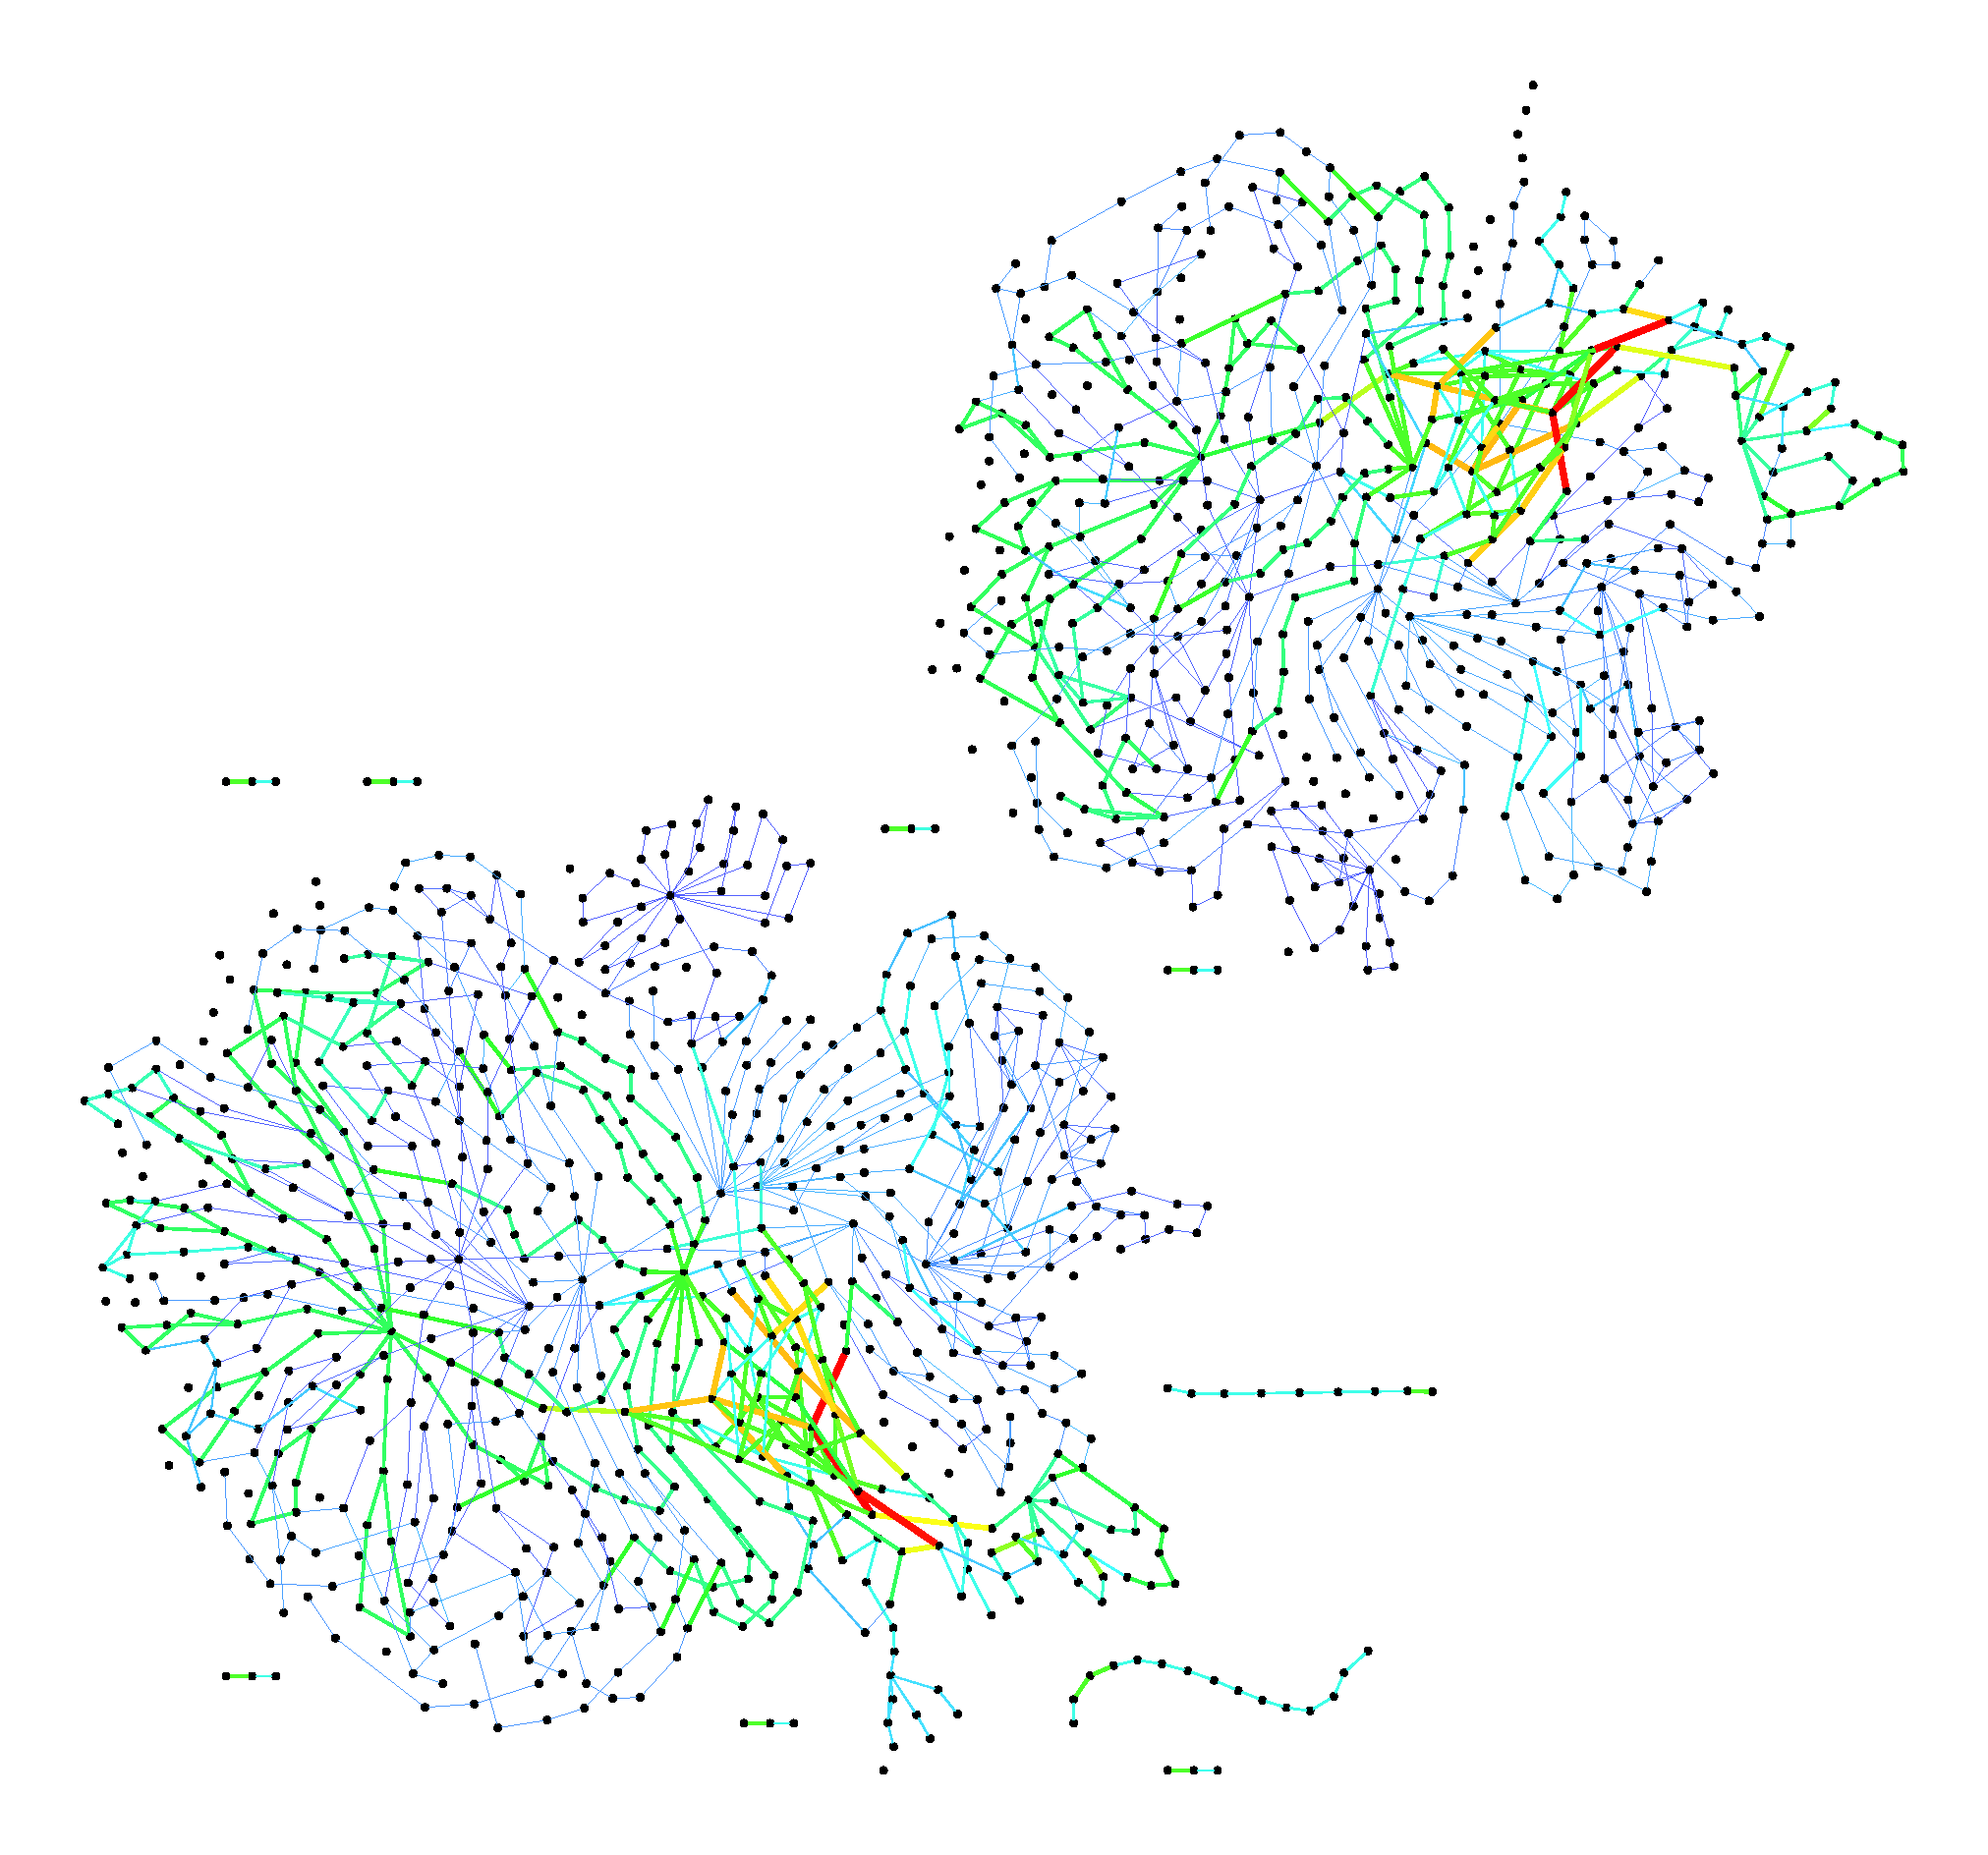
\includegraphics[clip=true,width=0.5\textwidth]{figs/s9234}
\caption{Heatmap of messages sent during the ISCAS'89 s9234 simulation}
\end{figure}

\begin{figure}[h]\label{fig:s9234_histo}
\centering
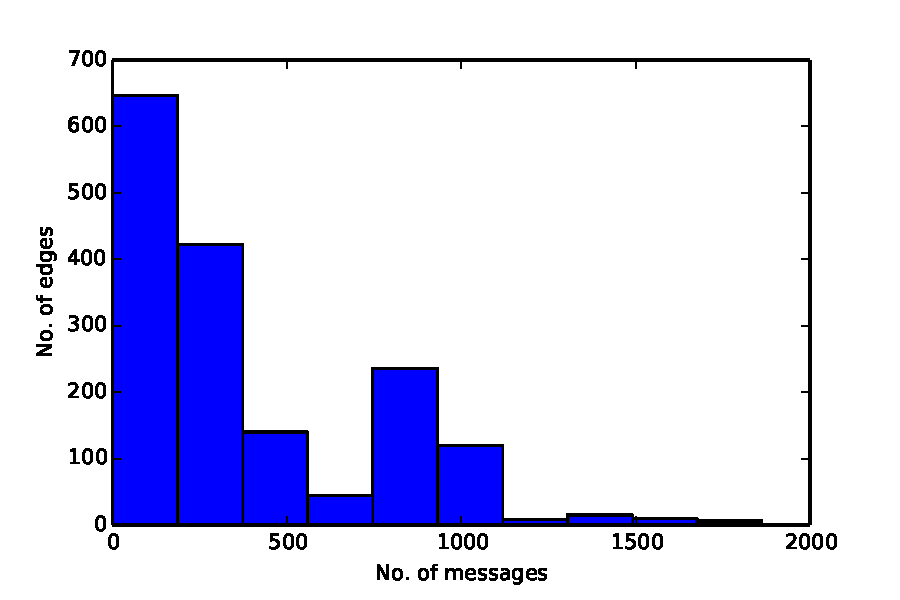
\includegraphics[clip=true,width=0.5\textwidth]{figs/s9234_histo}
\caption{Histogram of edge weights for ISCAS'89 s9234 simulation}
\end{figure}

\section{Partitioning Statistics Graphs}

The problem of partitioning the graph \(G\) into \(k\) partitions is referred to as \emph{k-way partitioning}. The goal is to partition the set of vertices \(V\) into the subsets \(V_1, V_2, \ldots, V_k\), with the constraint that \(V_i \cap V_j = \emptyset\) when \(i \neq j\). In order to balance load effectively, it is desirable to choose partitions such that \(|V_i|=n/k\). Additionally, the number of edges with incident vertices in different partitions should be minimized.

The library chosen to perform this partitioning is METIS, which is capable of performing multilevel recursive bisection and multilevel k-way partitioning on graphs \cite{karypis-98}. Several other partitioning libraries were considered, including PaToH, by Catalyürek and Aykanat \cite{catalyurek-11}; Chaco, by Hendrickson \cite{hendrickson-94}; and Scotch, by Chevalier and Pellegrini \cite{chevalier-08}. Ultimately, METIS was chosen due to its highly compatible ANSI C implementation, its open licensing, and its impressive performance, both in speed and in quality of partitions.

Of the various partitioning algorithms supported by METIS, its multilevel k-way partitioning algorithm was chosen due the high quality partitions produced. This algorithm works by \emph{coarsening} the graph by collapsing vertices and edges together to successively reduce its size. Once the size of the graph has been reduced to a small enough size, the small graph is partitioned and then uncoarsened into a partition of the original graph \cite{karypis-98}.

Multilevel k-way partitioning can achieve very good results. Figure~\ref{fig:s5378_4rr} shows the model from Figure~\ref{fig:s9234} partitioned into four partitions using a random algorithm that distributes the objects evenly between partitions in a round-robin manner, without regard to any graph edges. This random algorithm results in a graph in which \(75.83\%\) of edges weights cross between partitions. In contrast, Figure~\ref{fig:s5378_4part} shows the same graph partitioned into four partitions using the multilevel k-way algorithm described above. In this case, only \(1.38\%\) of edge weights cross between partitions. Graphs of all models studied in this thesis can be found in Appendix~\ref{appendixA}.

\begin{figure}[ht]\label{fig:s5378_4rr}
\centering
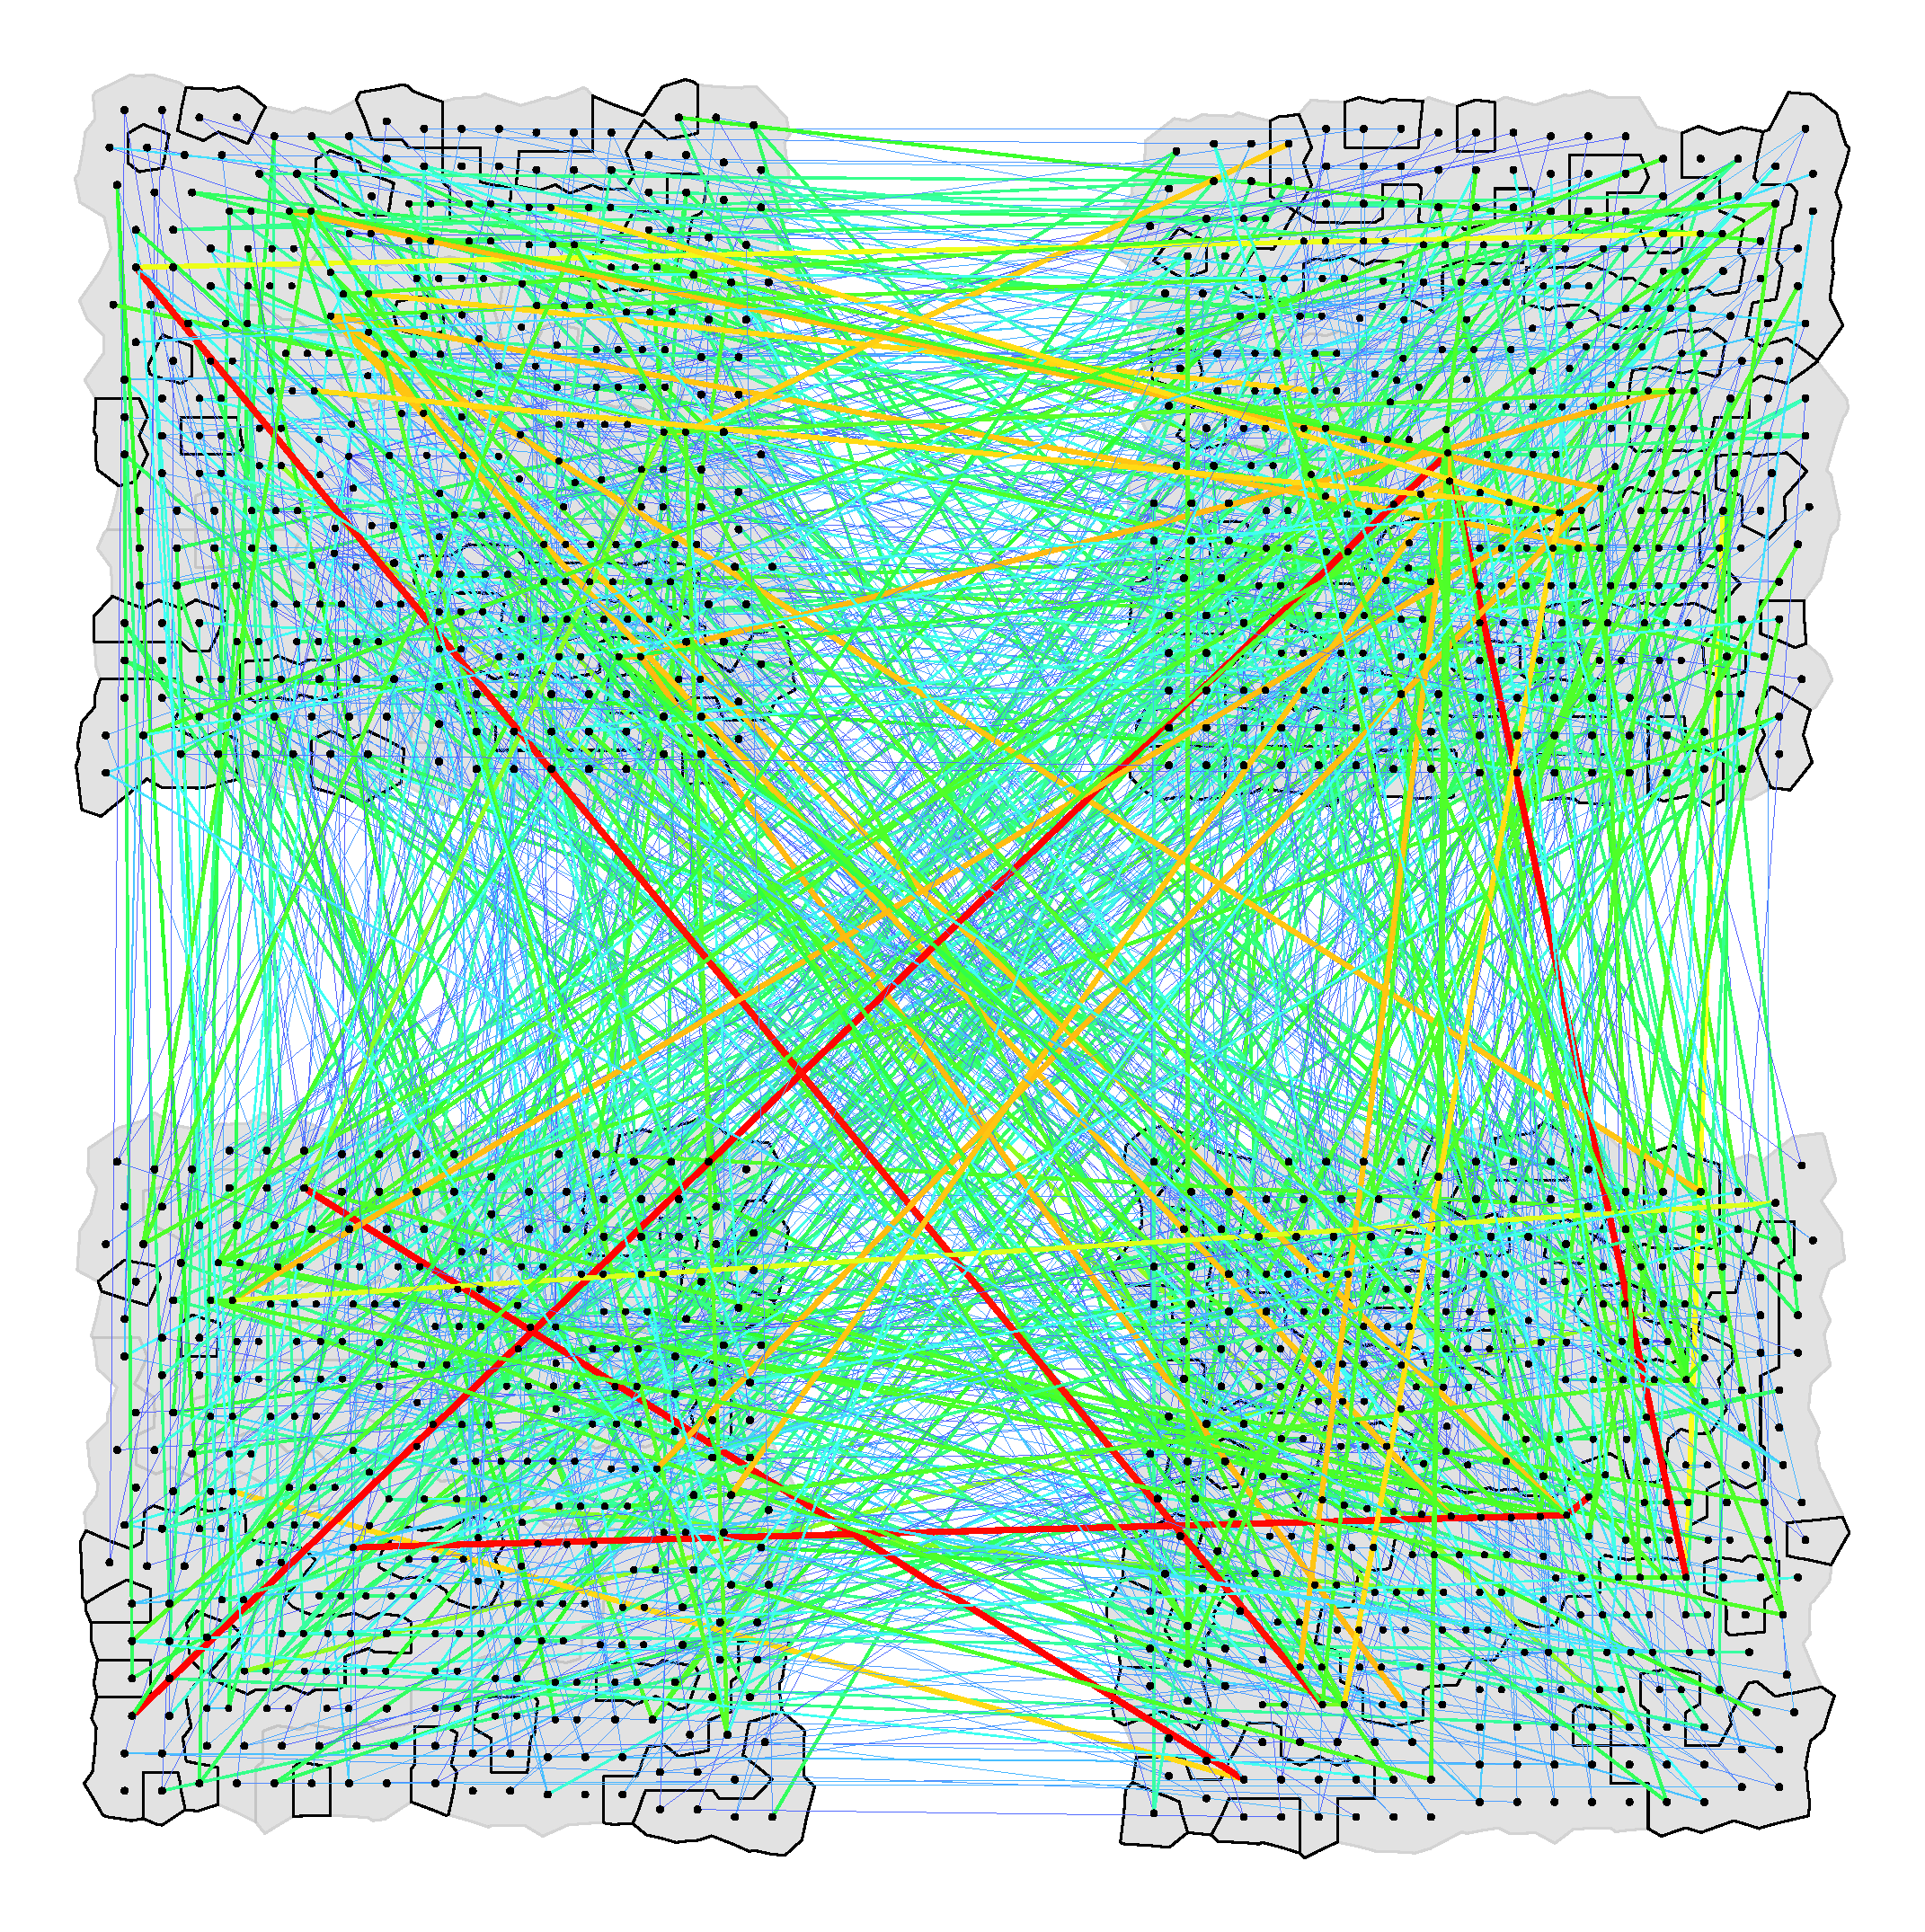
\includegraphics[clip=true,width=0.5\textwidth]{figs/s9234_4rr}
\caption{Heatmap of messages sent during the ISCAS'89 s9234 simulation, partitioned randomly into four partitions}
\end{figure}

\begin{figure}[ht]\label{fig:s5378_4part}
\centering
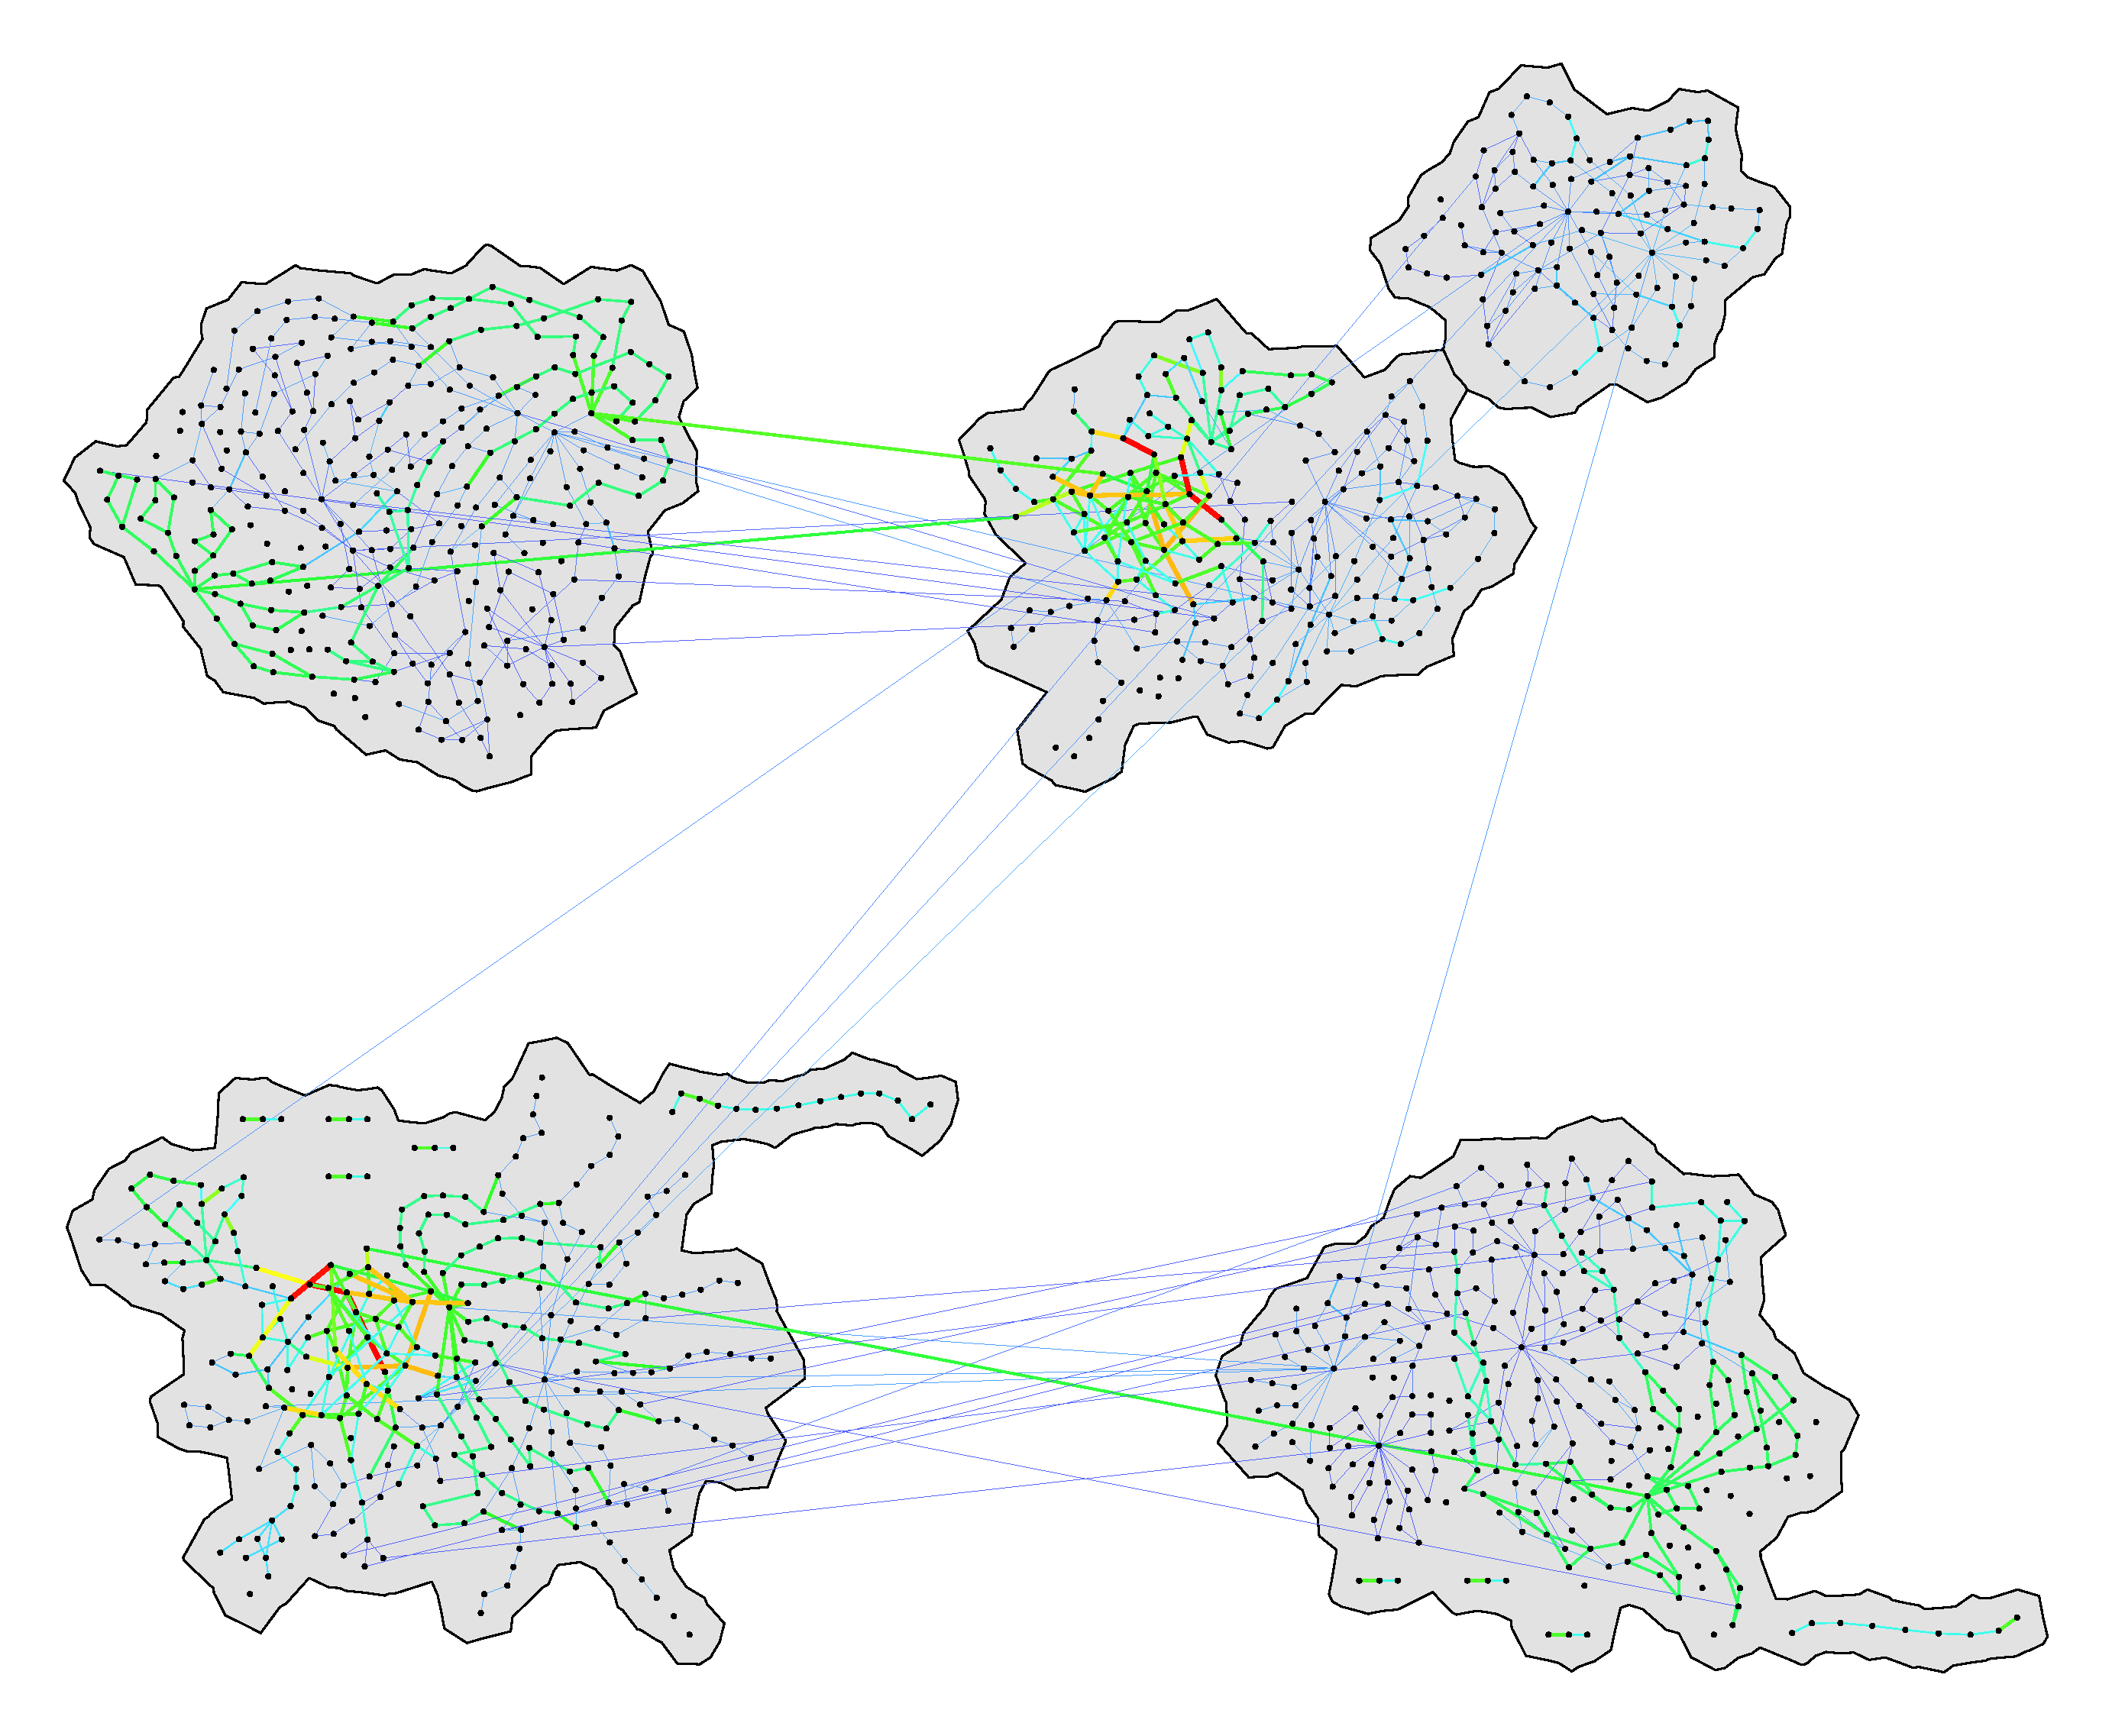
\includegraphics[clip=true,width=0.5\textwidth]{figs/s9234_4part}
\caption{Heatmap of messages sent during the ISCAS'89 s9234 simulation, partitioned into four partitions using the profile guided algorithm}
\end{figure}

\chapter{Implementation Details}\label{implementationDetails}

This chapter describes the details of the implementation of Profile Guided Partitioning in the \textsc{warped} kernel. In the first section, the user procedure for using the Profile Guided Partitioning is outlined. In the following section, the method used to collect statistics is detailed. Finally, the modifications to the \textsc{warped} kernel required for run-time configurable partitioning are described and the details of profile guided partitioning in \textsc{warped} are given.

\section{Procedure for Using Profile Guided Partitioning in \textsc{warped}}

To use the Profile Guided Partitioning functionality in \textsc{warped}, a two-step process was chosen. First, profile data is collected during a sequential simulation run and stored in an intermediate file on disk. This statistics file is then read by \textsc{warped} when run in a parallel configuration in order to perform partitioning. It would be possible to perform profiling automatically in one step, which would save a small amount of user intervention, but there are a number of drawback to automatic partitioning that led to the choice of the current procedure.

Firstly, profiling takes time. By saving the results to disk a user is able to perform profiling once, then use the collected data for multiple runs. Because the profiling data is independent of the platform used, including the number of simulation nodes, a benchmarking run consisting of multiple system configurations only needs to perform profiling once

Of course, it would be possible to cache the profiling results between simulation runs, even if the profiling was performed automatically. However, the one-step process still has a larger drawback. Some simulation models have a natural termination condition. For example, a VLSI circuit model might read in a fixed-length input vector and terminate once all inputs have propagated through the circuit. Not all models terminate naturally, however. A model of a disease epidemic spreading through a geographic area may not have a natural termination condition. Instead, this model would run until a given GVT value was reached. Even if a model does have a natural termination condition, it may be a very long running simulation. In this case, it is desirable to terminate at a given GVT to save time. Either way, an automated one-step profiling procedure would not be able to automatically determine the termination settings. Because of this, the two-step process in advantageous.

\section{Collecting Profiling Data}\label{sec:collectingProfilingData}

All statistics are collected using the \texttt{GraphStatistics} class in \textsc{warped}. This class implements an undirected graph which can record multiple weights per edge. It supports writing the collected statistics to disk in two different file formats. The first is a Graphviz compatible graph description that can be used to visualize the results. The second is a modification of the graph file format defined by METIS \cite{karypis-11}, and is the format used to perform partitioning. The METIS file format needed to be modified to account be able to map the vertices in the graph back to the corresponding \texttt{SimulationObject}. When the \texttt{SimulationObject}s are created, they are assigned \texttt{OBJECT\_ID}s deterministically. If all objects appeared exactly once in the graph, the vertices could be mapped back to \texttt{SimulationObjects} sequentially without extra information. However, in some models, it is possible that an object never sends or receives events from other objects during the profiling run. METIS does not support vertices with no connected edges, so the object is not recorded in the statistics graph. To compensate for this, comments are inserted into the graph file indicating the \texttt{OBJECT\_ID} of each vertex.

Statistics are collected when \textsc{warped} is configured to use the \texttt{SequentialSimulationManager}. During simulation, the manager records each event that an object sends, incrementing the corresponding edge weight on the graph. It is possible that an object may send an event to itself. These events are legal, but have no effect on partitioning, and so are not recorded. At the end of the simulation, the graph is written to disk. Because the manager simply records the events that are sent during simulation, it requires no knowledge of the model, and so works with all models.


\section{Profile Guided Partitioning in \textsc{warped}}

Prior to this thesis, all partitioning was performed by the \texttt{Application} classes, and so was not configurable. Each \texttt{Application} implementation had to define a method \texttt{getPartitionInfo} that took as a parameter a number of partitions, and returned a number of \texttt{std::vector}s equal to the number of partitions, with each \texttt{std::vector} populated with \texttt{SimulationObjects}. This interface, which combined the act of creating \texttt{SimulationObjects} and partitioning them, was simple to implement. However, it prevented \textsc{warped} from performing its own partitioning, and forced all models to implement their own partitioning algorithm.

To enable run-time configurable partitioning, the \texttt{Application} interface was modified. The act of creating \texttt{SimulationObjects} was moved to a new method, \texttt{getSimulationObjects}, that returns an unpartitioned \texttt{std::vector} of \texttt{SimulationObject}s. Models still have the option of defining custom partitioning by implementing the \texttt{getPartitionInfo} method. This which is now optional and takes as a parameter the previously created \texttt{std::vector} of \texttt{SimulationObject}s.

The class \texttt{PartitionManager} was created to support run time partitioning. Depending on how \textsc{warped} is configured, the \texttt{PartitionManager} will delegate to the custom partitioning algorithm written by the models, if any, or it can ignore the custom algorithm and use one of several built-in algorithms, including the profile guided partitioning algorithm.

The profile guided partitioning algorithm is implemented in the \texttt{ProfileGuidedPartitioner} class. This class reads the graph file described in Section~\ref{sec:collectingProfilingData}. The METIS library is used to perform k-way partitioning on the graph, and the partitioning information is used to assign \texttt{SimulationObject}s to partitions. Any \texttt{SimualtionObject}s not appearing in the graph are assigned evenly to all partitions.

\chapter{Performance Analysis}\label{analysis}

This chapter discusses the performance results of experiments on the Profile Guided Partitioning algorithm implemented in the \textsc{warped} PDES kernel. The first section explains the objectives of the analysis. The next two sections discuss the simulation models used in this analysis. The final section presents the data obtained from the experiments.

\section{Objectives}

The first objective of this analysis is to determine the effectiveness of the Profile Guided Partitioning algorithm in reducing the run time of \textsc{warped} simulations versus the standard naive algorithm. The second objective is to determine if Profile Guided Partitioning is effective on various types of simulation models without using any model-specific knowledge.

\section{The ISCAS'89 Simulation Model}

In 1989, the International Symposium on Circuits and Systems released a set of digital circuit descriptions named the ISCAS'89 Benchmarks. These circuits have been widely used as a standard set of circuits to study VLSI systems and simulators. The benchmark consists a number of circuits of varying sizes and complexities. Each circuit description is a list of components including inputs, outputs, logic gates (AND, NOT, NOR, etc.), and D Flip-Flops. The connections for all components are given, with many logic gates having more than two inputs. For this thesis, three of the ISCAS'89 circuits are studied: s5378, s9234, and s38584.1. Although high-level descriptions for most ISCAS'89 circuits do not exist, statistics on the components of each circuit can be found in Table~\ref{tab:iscasStats} \cite{brglez-89}.

\begin{table}[h]
\centering
\begin{tabular}{@{}llllll@{}}
\toprule
Circuit  & No. of Inputs & No. of Outputs & No. of Logic Gates & No. of Flip-Flops & Description    \\ \midrule
s5378    & 35            & 49             & 2779               & 179               & Unknown        \\
s9234    & 19            & 22             & 9772               & 597               & Real Chip Scan \\
s38584.1 & 38            & 304            & 19253              & 1426              & Real Chip Scan \\ \bottomrule
\end{tabular}
\caption{Characteristics of the ISCAS'89 benchmark circuits examined in this paper}
\label{tab:iscasStats}
\end{table}

\section{The RAID Simulation Model}\label{raidDiscussion}

The RAID model simulates a RAID-5 Disk Array \cite{hennessy-12}. RAID is an acronym for Redundant Array of Independent Disks, and is a set of algorithms for extending a logical storage volume across multiple physical disks. Each RAID algorithm is called a \emph{RAID level}, with each level providing increases in performance, data resiliency in the face of disk failure, or both. RAID-5 is a RAID level that provides both data resiliency and performance improvements by \emph{striping} data across multiple disks, and calculating parity information that can be used to reconstruct lost data in the case of disk failure. RAID arrays are typically ran through a \emph{RAID controller}, which is responsible for performing any calculations necessary to handle reading and writing to the array. The RAID simulation model supports modeling of multiple types of physical disks, as well as various configurations of controllers and processes that generate disk activity. The configuration used for performance analysis in this thesis consists of 32 Fujitsu disks, 8 controllers, and 96 processes.

\section{Experimental Results}

All benchmarks were run on a Beowulf cluster of quad-core, Hyper-Threaded Intel Xeon processors running at 2.33GHz. Simulations were run on 2, 4, and 8 nodes using both the Profile Guided Algorithm, and a random algorithm that distributes objects equally to each partition in a round-robin manner without using any extra information. Non-threaded \textsc{warped} was used in its default configuration for all benchmarks. Specifically, a periodic state manager with a period of ten was used. An aggressive cancellation strategy was used with default Anti-Messages. Optimistic Fossil Collection and DVFS were not used. MPICH2 version 1.4 was used as the MPI implementation. \textsc{warped} was built with the g++ compiler with the \texttt{-02} optimization flag.

The results are summarized in Table~\ref{tab:benchmarks}. Profile Guided Partitioning performs significantly better than naive partitioning in all cases, with the speedup ranging from \(1.59\times\) up to \(6.04\times\), depending on the configuration. In some models, the speed up increases with the number of nodes, while in others the speedup remains constant or decreases as the number of nodes increases.

\begin{table}[h]\label{tab:benchmarks}
\centering
\begin{tabular}{@{}lllll@{}}
\toprule
Model             & No. of Nodes & Random & Profile Guided & Speedup           \\ \midrule
ISCAS89: s5378    & 2            & 15.57  & 6.19           & \(2.51\times\)    \\
                  & 4            & 9.12   & 4.25           & \(2.15\times\)    \\
                  & 8            & 6.77   & 3.20           & \(2.11\times\)    \\ \midrule
ISCAS89: s9234    & 2            & 64.76  & 10.73          & \(6.04\times\)    \\
                  & 4            & 35.39  & 7.23           & \(4.89\times\)    \\
                  & 8            & 23.23  & 13.37          & \(1.74\times\)    \\ \midrule
ISCAS89: s38584.1 & 2            & 64.92  & 40.92          & \(1.59\times\)    \\
                  & 4            & 28.05  & 11.76          & \(2.39\times\)    \\
                  & 8            & 13.25  & 3.87           & \(3.42\times\)    \\ \midrule
RAID              & 2            & 103.79 & 20.41          & \(5.09\times\)    \\
                  & 4            & 46.16  & 9.78           & \(4.72\times\)    \\
                  & 8            & 26.22  & 4.86           & \(5.40\times\)    \\ \bottomrule
\end{tabular}
\caption{Simulation Run Time (in seconds) and Speedup for the different partitioning algorithms}
\end{table}

The differences in scaling of speedup factors across the different models are significant. The fact that the scaling differs so significantly even for different circuits of the same ISCAS model suggests that the structure of the statistics graph --- and hence the structure of the simulation --- is the primary factor in determining the potential performance. Graphs of all models used can be found in Appendix~\ref{appendixA}.

The speedup gained by using Profile Guided Partitioning on the RAID model is fairly independent of the number of nodes used, remaining around \(5\times\) for all tested number of nodes. This is logical based on the structure of the RAID model. Each RAID controller is connected to a number of disks and processes that communicate with each other. However, each controller and its associated disks and processes form a cluster of objects which does not communicate with other clusters. Because of this regular, disjoint structure, it is possible to partition the simulation such that no events cross partition boundaries.

The various ISCAS circuits present more complicated graphs, and show a variety of speedup scaling behaviors. Due to the fact that the ISCAS model is based on real-world circuits, the graphs are much less regular than the RAID benchmark. Table~\ref{tab:eventCrossings} shows the percentage of events crossing partition boundaries for the various models. With Profile Guided Partitioning, the number of events crossing partitions increases by a small, consistent amount as the number of partitions increases. The scaling of performance, however seem uncorrelated to the scaling of the fraction of events crossing partitions.

\begin{table}\label{tab:eventCrossings}
\centering
\begin{tabular}{@{}llll@{}}
\toprule
Model              & No. of Nodes & Random  & Profile Guided \\ \midrule
ISCAS'89: s5378    & 2            & 49.56\% & 1.95\%         \\
                   & 4            & 75.16\% & 3.86\%         \\
                   & 8            & 89.07\% & 6.54\%         \\ \midrule
ISCAS'89: s9234    & 2            & 48.91\% & 0.15\%         \\
                   & 4            & 72.76\% & 0.94\%         \\
                   & 8            & 86.93\% & 2.95\%         \\ \midrule
ISCAS'89: s38584.1 & 2            & 49.38\% & 0.17\%         \\
                   & 4            & 75.33\% & 0.61\%         \\
                   & 8            & 87.29\% & 1.16\%         \\ \midrule
RAID               & 2            & 49.24\% & 0.00\%         \\
                   & 4            & 73.88\% & 0.00\%         \\
                   & 8            & 86.19\% & 0.00\%         \\ \bottomrule
\end{tabular}
\caption {Recorded fraction of events crossing partitions for various models and partitioning strategies}
\end{table}

\begin{figure}
\centering
\benchbar{103.79}{46.16}{26.22}{20.41}{9.87}{4.86}
\caption {Run time of RAID simulation}
\end{figure}

\begin{figure}
\centering
\benchbar{15.56}{9.12}{6.76}{6.19}{4.24}{3.20}
\caption {Run time of ISCAS'89 simulation using the s5378 circuit}
\end{figure}

\begin{figure}
\centering
\benchbar{64.76}{35.39}{23.23}{10.73}{7.23}{13.37}
\caption {Run time of ISCAS'89 simulation using the s9234 circuit}
\end{figure}

\begin{figure}
\centering
\benchbar{64.92}{28.05}{13.25}{40.92}{11.76}{3.87}
\caption {Run time of ISCAS'89 simulation using the s38584.1 circuit}
\end{figure}

\chapter[Conclusions \& Future Research]{Conclusions and Suggestions for Future Research}\label{conclusion}

This chapter presents conclusions for the research presented in this thesis. This first section gives a summary of the results. The second section discusses some possibilities for future research based on this thesis.

\section{Summary of Findings}

The performance of Profile Guided partitioning was measured relative to a naive partitioning algorithm for a number of simulation models. The models included a simulation of a RAID disk array, and a number of digital circuits that are part of the ISCAS'89 benchmark. All simulations were run on an Intel Xeon Beowulf cluster.

The Profile Guided Partitioning algorithm was found to perform significantly better than the naive algorithm, with certain configurations exhibiting up to a six-fold speedup. The runtime of all models scales well when run with the Profile Guided Partitioning algorithm, although the speedup over the naive algorithm is inconsistent. The speedup of the Profile Guided Partitioning over the naive algorithm increases for some models as the number of partitions increases, while the speedup decreases for some models. However, even the worst speedup is still a \(1.59\times\) improvement.

\section{Suggestions for Future Work}

The inconsistent speedups seen in the various simulation models invites more investigation. There are a number of possible explanations for this behavior. It is possible that performance speedups could be made more consistent if a different statistic was used to assign weights to the edges in the profiling graph. Because rollbacks are a significant source of slowdown in PDES \cite{fujimoto-90}, a different profiling statistic may serve to reduce rollbacks further than the count of events used in this thesis. For example, it may be the case that events sent farther into the future may have a lower probability of causing a rollback than an event that is scheduled to occur soon after it was created. In this case, it may be beneficial to assign higher weights to events that have a shorter delay.

Since it is possible to collect statistics on a short run of a simulation, then use these gathered statistics to partition a longer simulation run, it would also be worth investigating the relationship between the length of the profiling run and the performance of the final simulation. This relationship would be extremely dependent on the model, however. Simulation models that exhibit steady-state behavior, such as the RAID simulation presented in Section~\ref{raidDiscussion}, would likely only need a very small amount of profiling. In contrast, models that exhibit dynamic behavior over the course of a simulation would likely perform poorly when partitioned with an insufficient amount of profiling data.

\bibliography{refs}
\bibliographystyle{ieeetr} \markright{ }

\appendix
\chapter{Graphs of Partitioned Models}\label{appendixA}

This appendix captures the heatmap images of the simulation models used in the
investigations of this thesis. In particular, sets of heatmap images for the following
simulation models are presented:


\begin{enumerate}

  \item RAID,
  \item s5378 (from the ISCAS '89 model set),
  \item s9234 (from the ISCAS '89 model set), and
  \item s38584 (from the ISCAS '89 model set).

\end{enumerate}

\noindent

For each model, four images are shown that correspond to: (i) an unpartitioned configuration, (ii) a two partition configuration, (ii) a four partition configuration, and (iv) an eight partition configuration. The partitions are generated by the METIS software as discussed in Chapter 4. The partitions shown are exactly the partitions used in the performance analysis results discussed in Chapter 6.

\begin{figure}
\centering
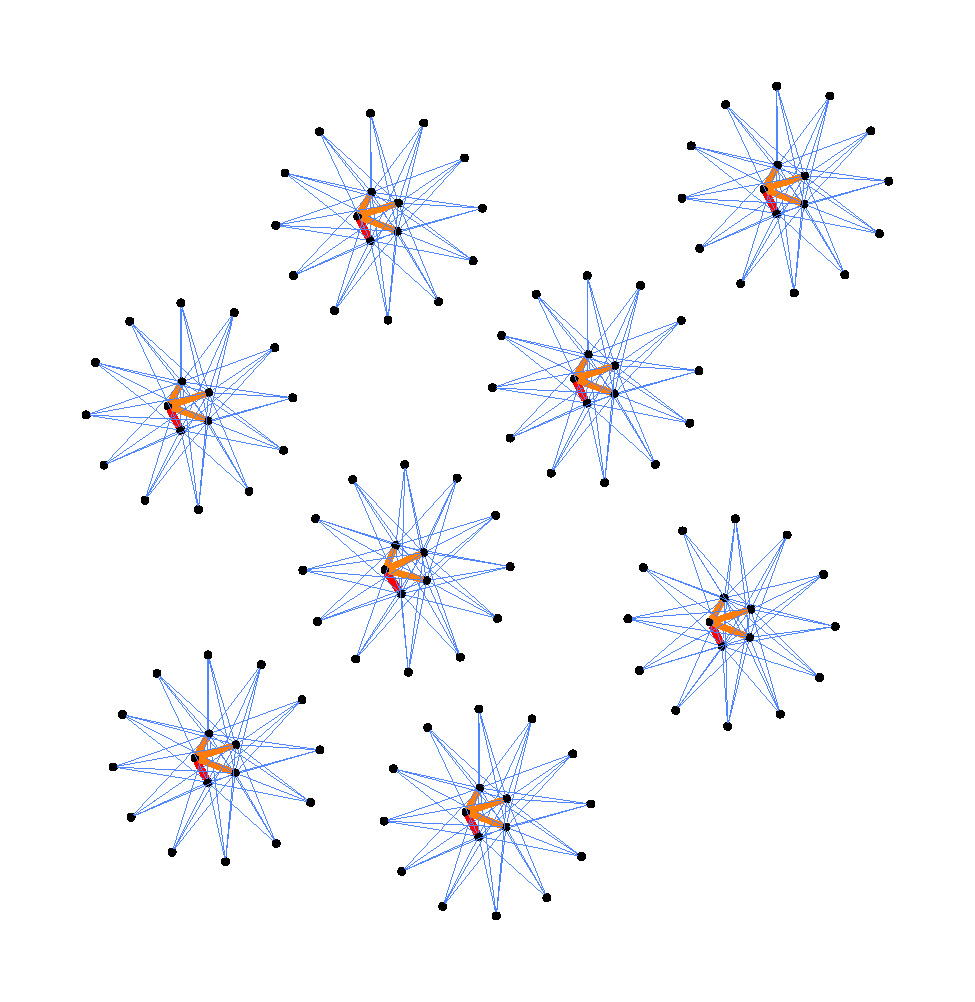
\includegraphics[width=\textwidth,height=0.9\textheight,keepaspectratio]{figs/RAID}
\caption{Heatmap of messages sent during the RAID simulation.}
\end{figure}

\begin{figure}
\centering
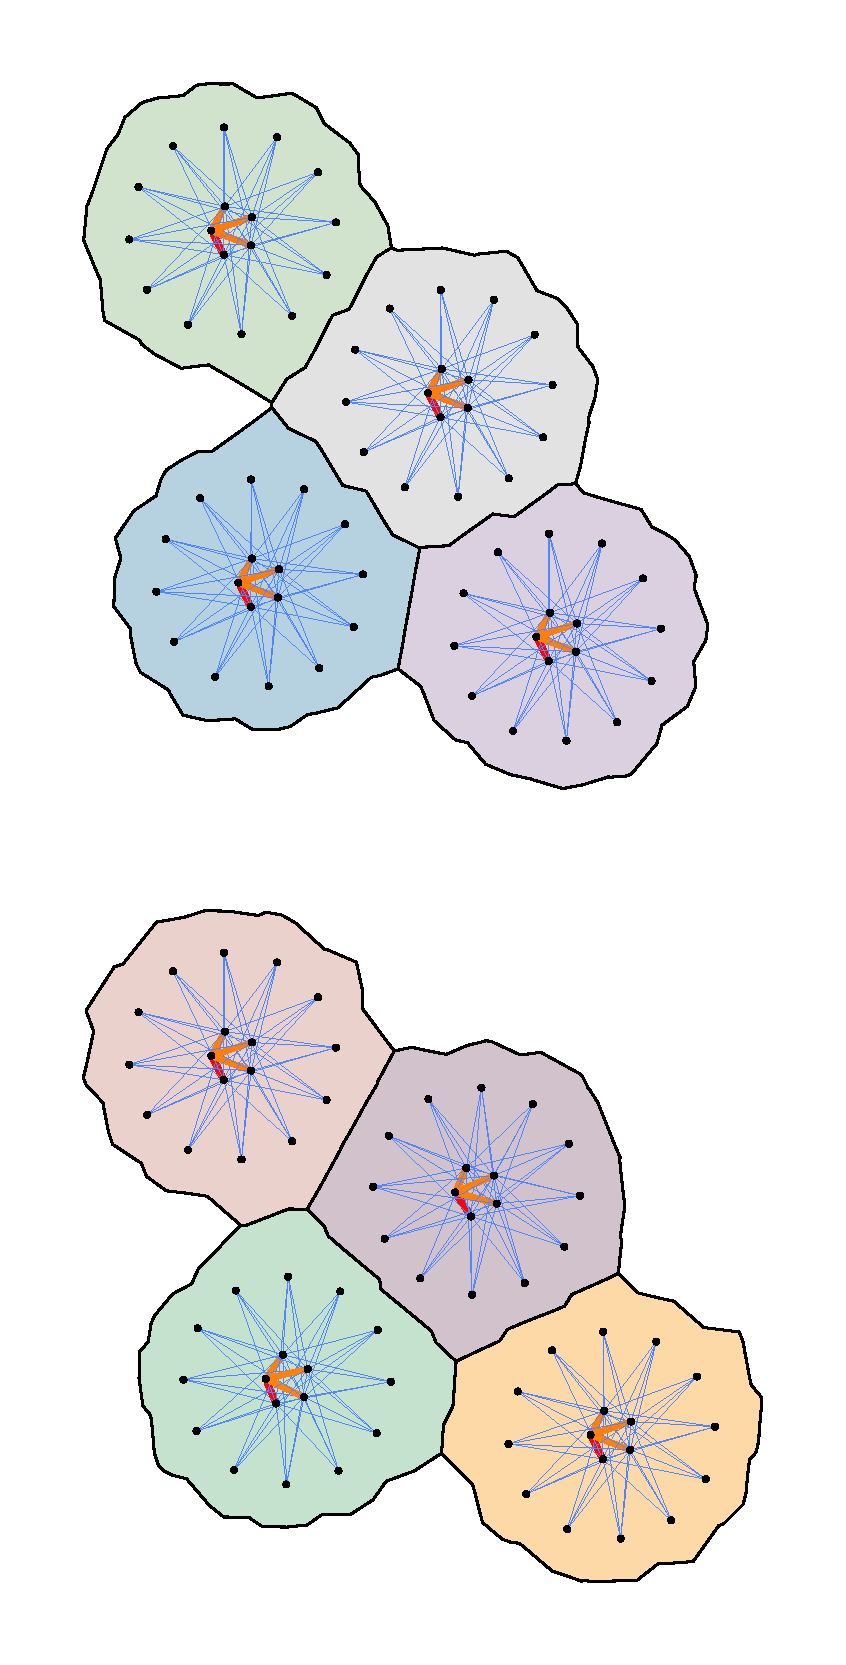
\includegraphics[width=\textwidth,height=0.9\textheight,keepaspectratio]{figs/RAID_2part}
\caption{Heatmap of messages sent during the RAID simulation, partitioned into two partitions using the profile guided algorithm.}
\end{figure}

\begin{figure}
\centering
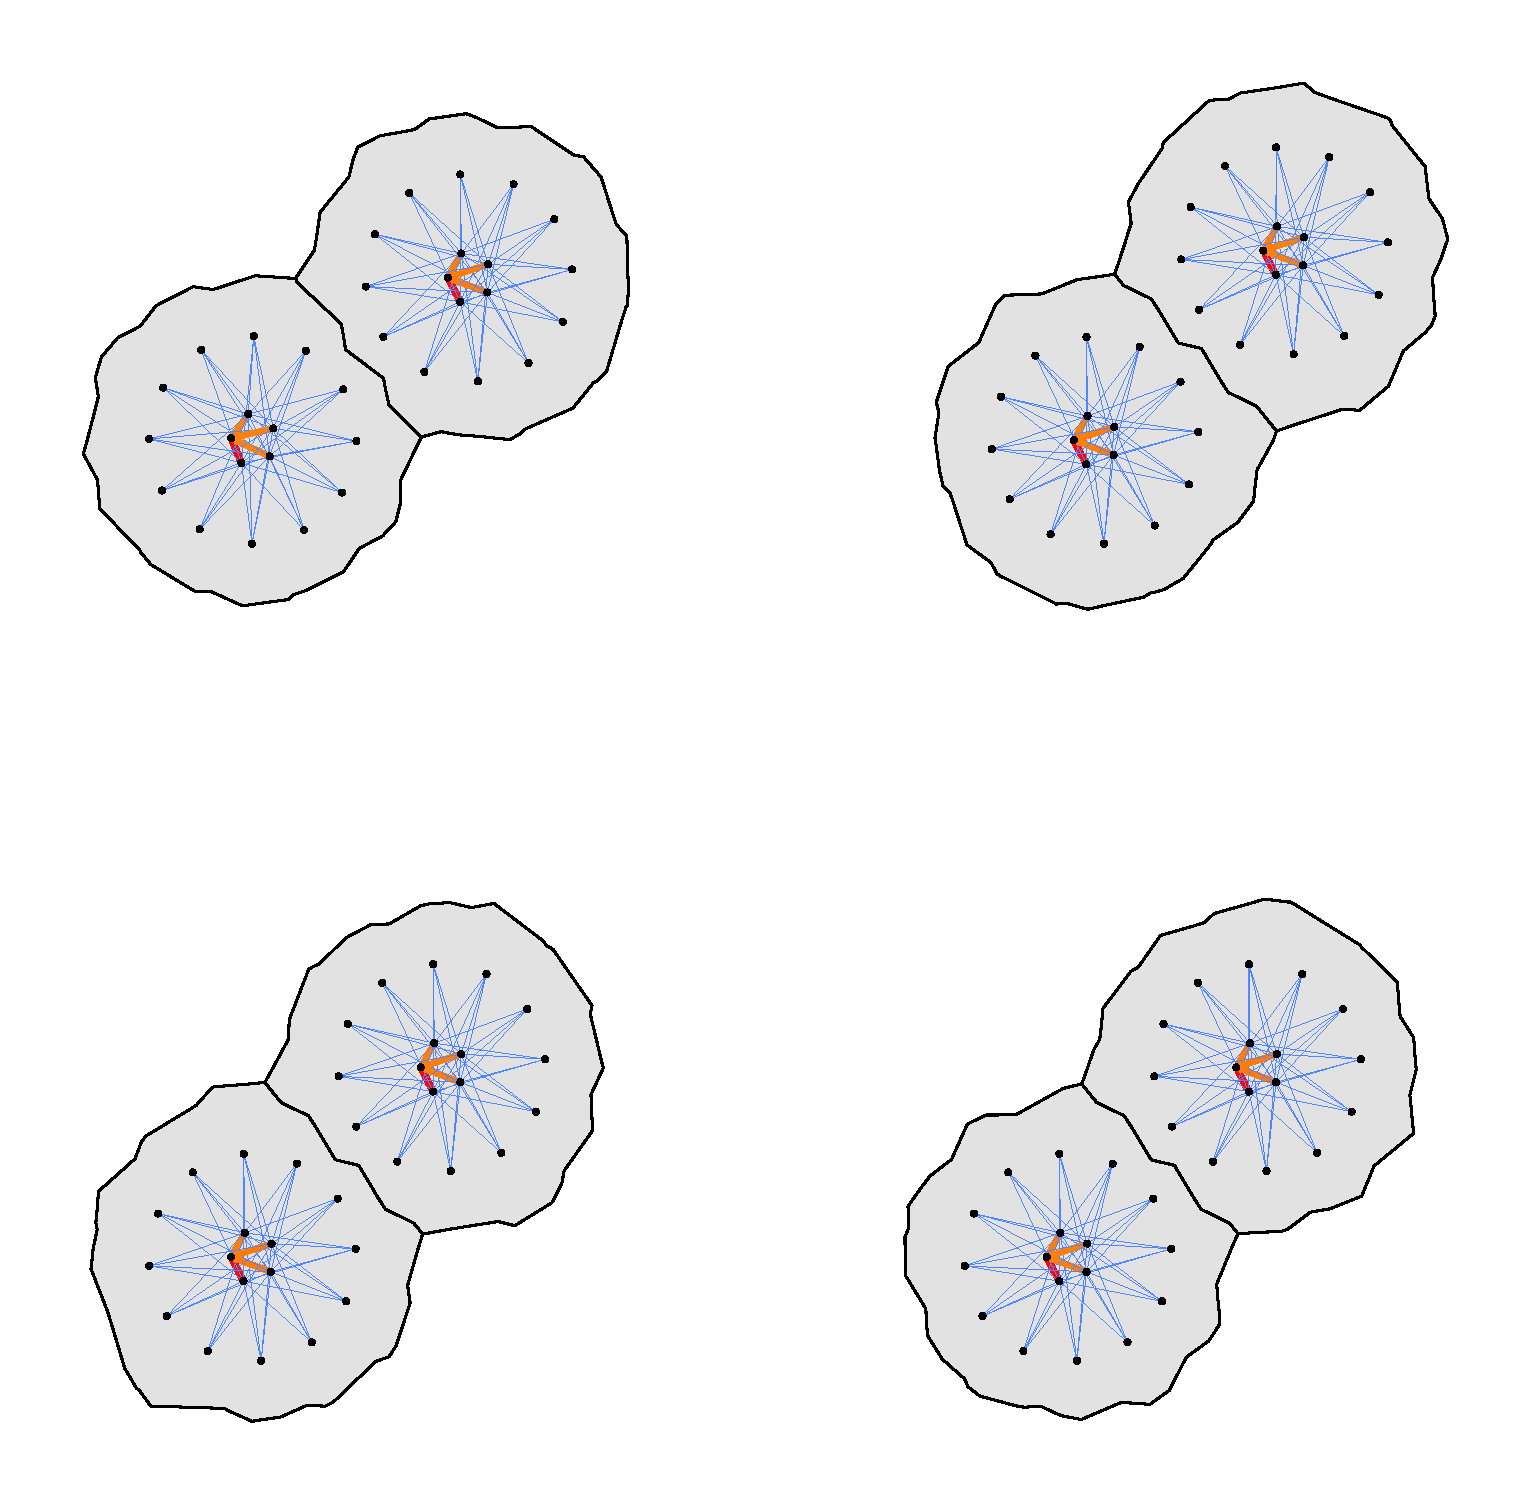
\includegraphics[width=\textwidth,height=0.9\textheight,keepaspectratio]{figs/RAID_4part}
\caption{Heatmap of messages sent during the RAID simulation, partitioned into four partitions using the profile guided algorithm.}
\end{figure}

\begin{figure}
\centering
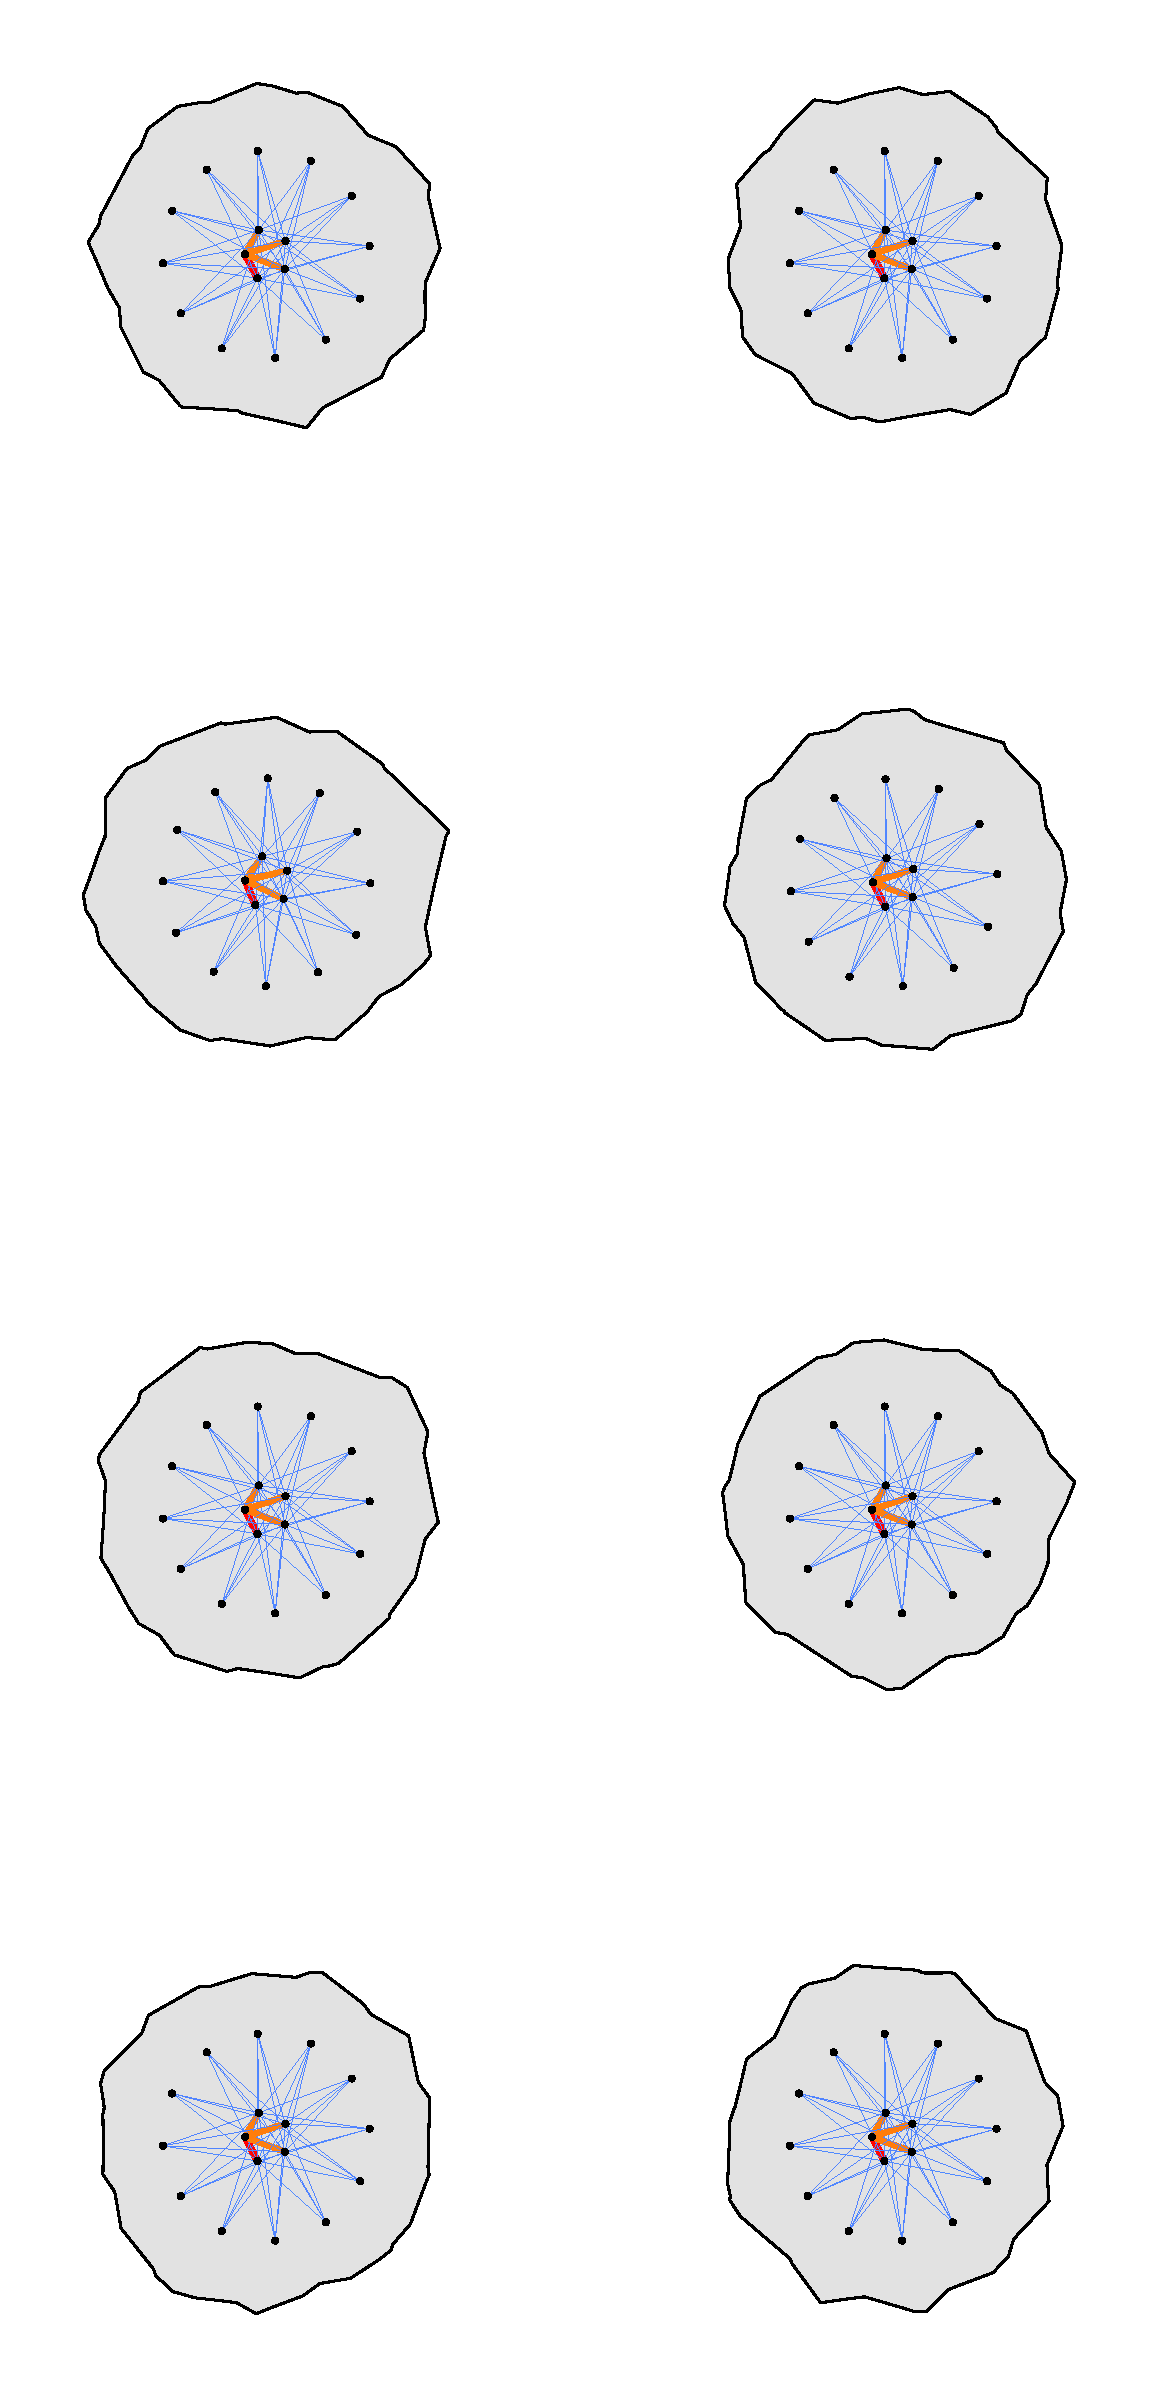
\includegraphics[width=\textwidth,height=0.9\textheight,keepaspectratio]{figs/RAID_8part}
\caption{Heatmap of messages sent during the RAID simulation, partitioned into eight partitions using the profile guided algorithm.}
\end{figure}

\begin{figure}
\centering
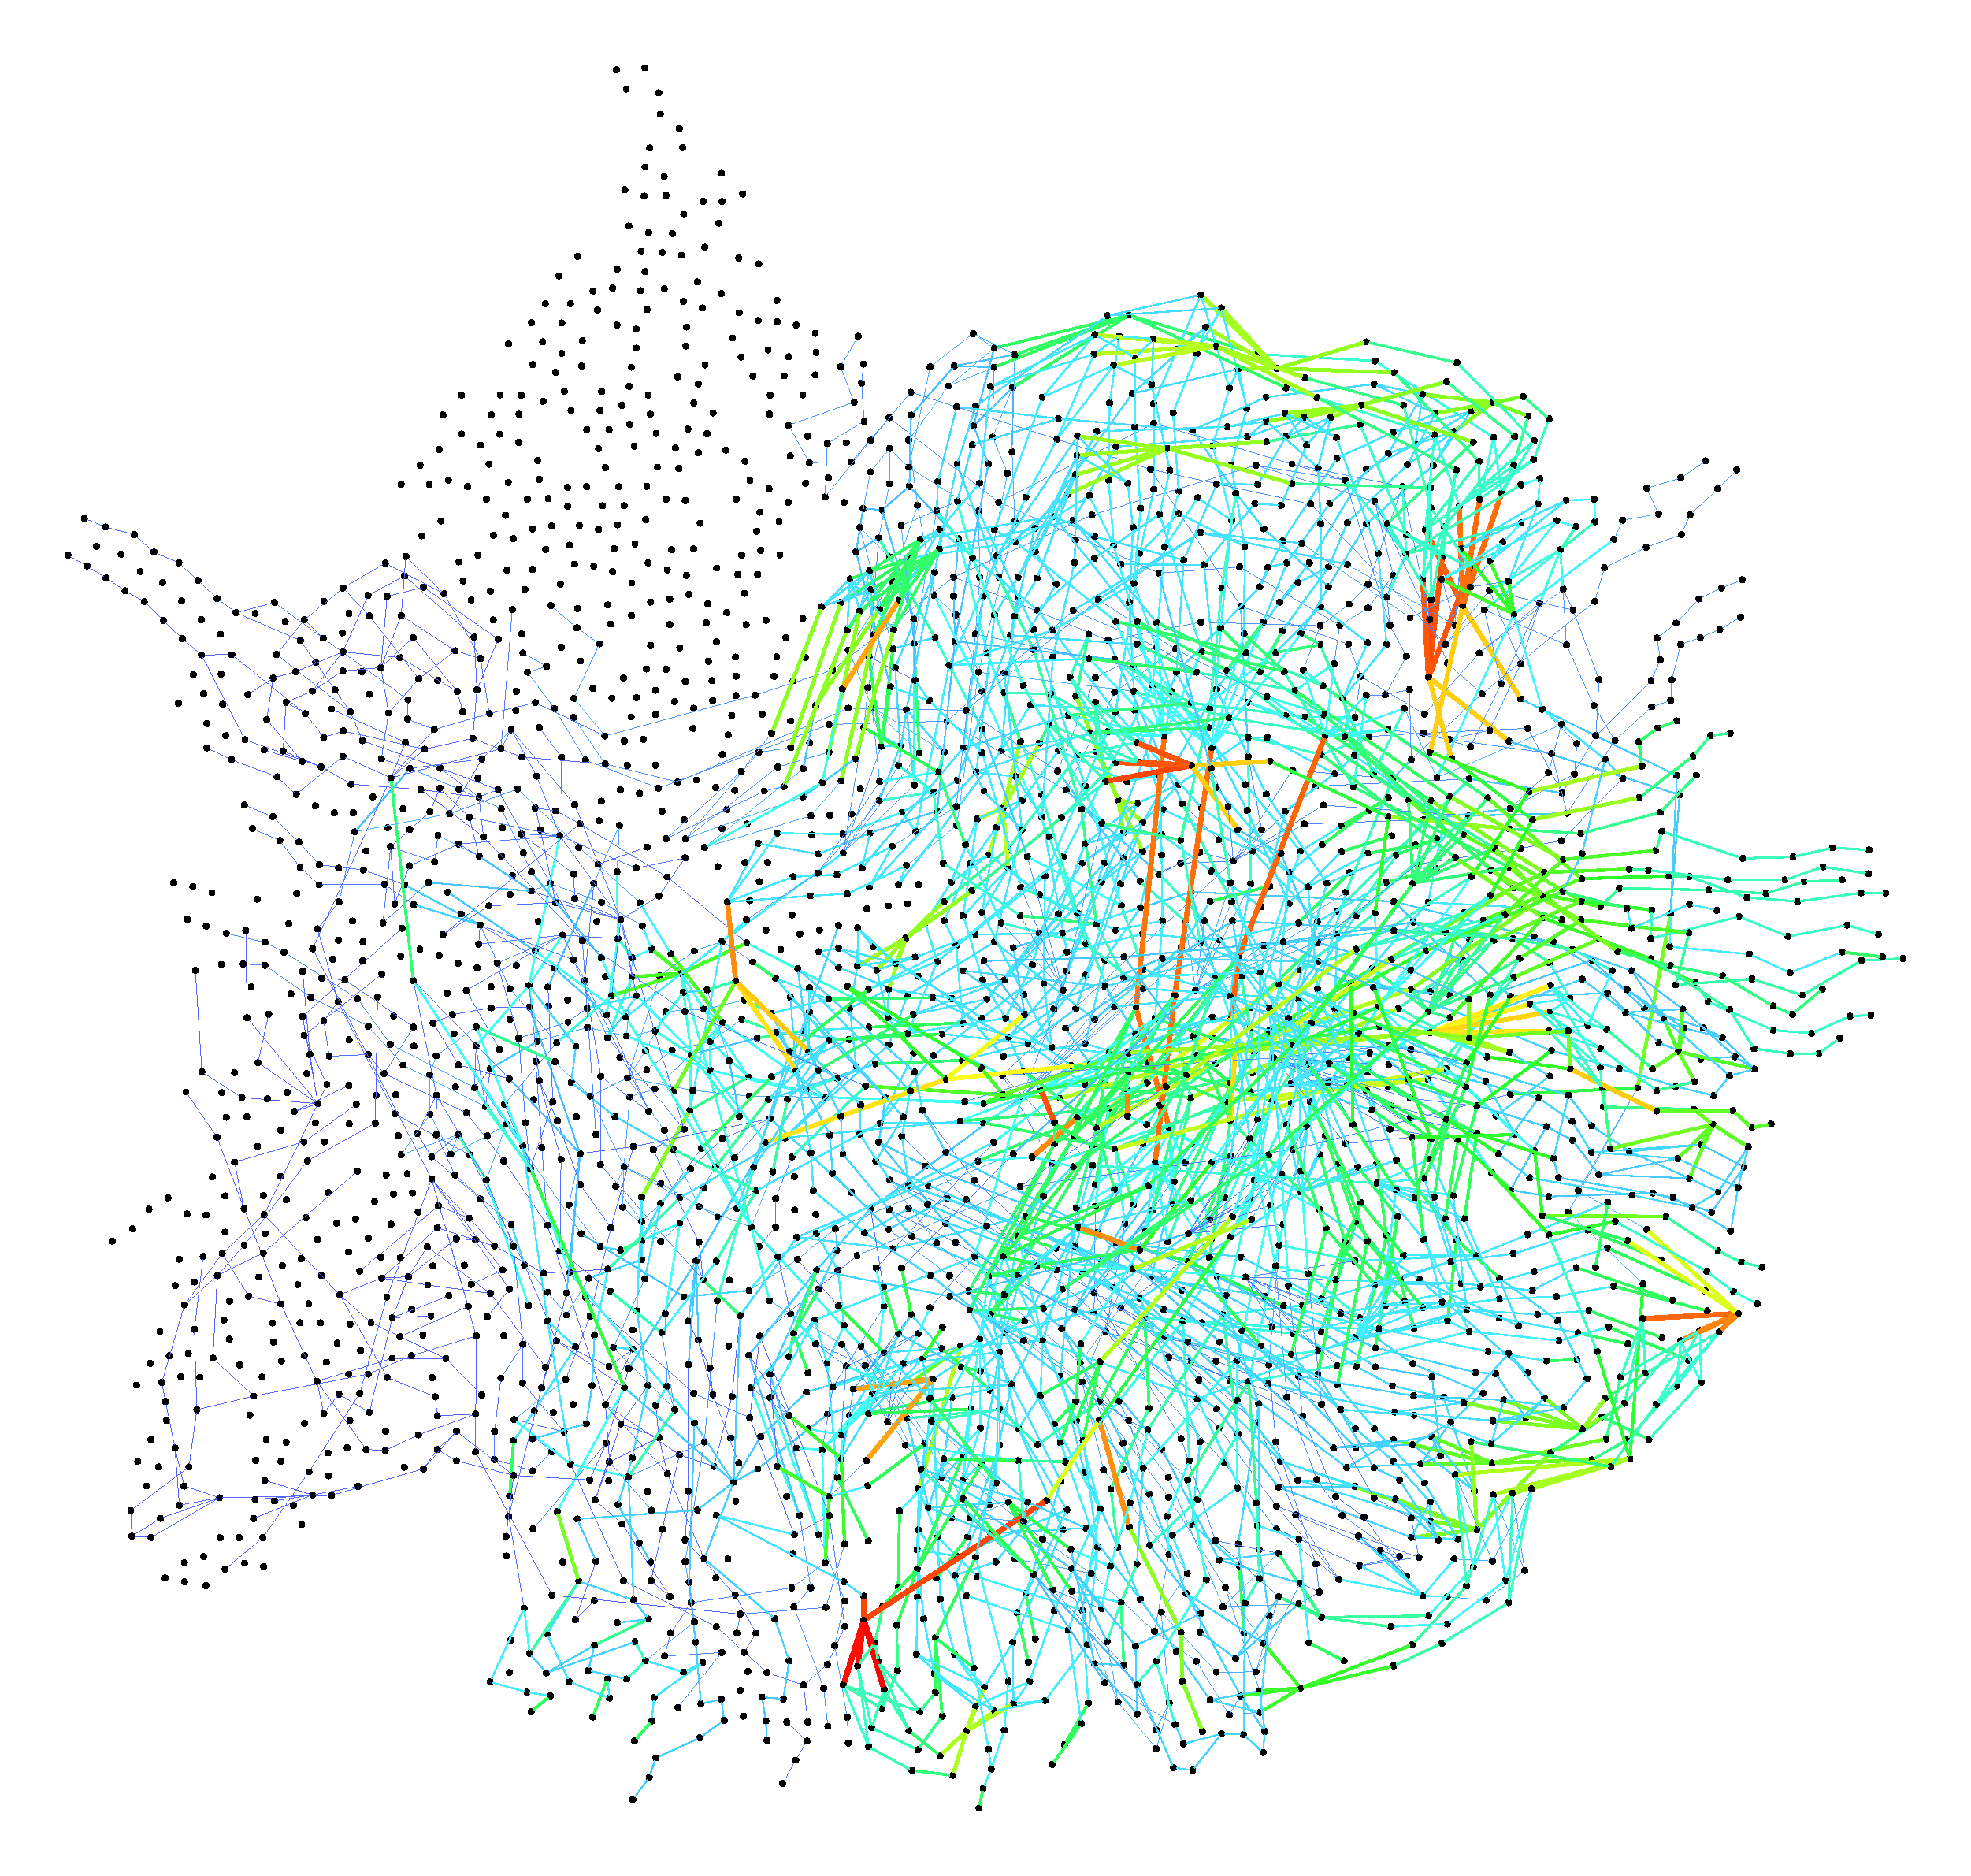
\includegraphics[width=\textwidth,height=0.9\textheight,keepaspectratio]{figs/s5378}
\caption{Heatmap of messages sent during the ISCAS'89 s5378 simulation.}
\end{figure}

\begin{figure}
\centering
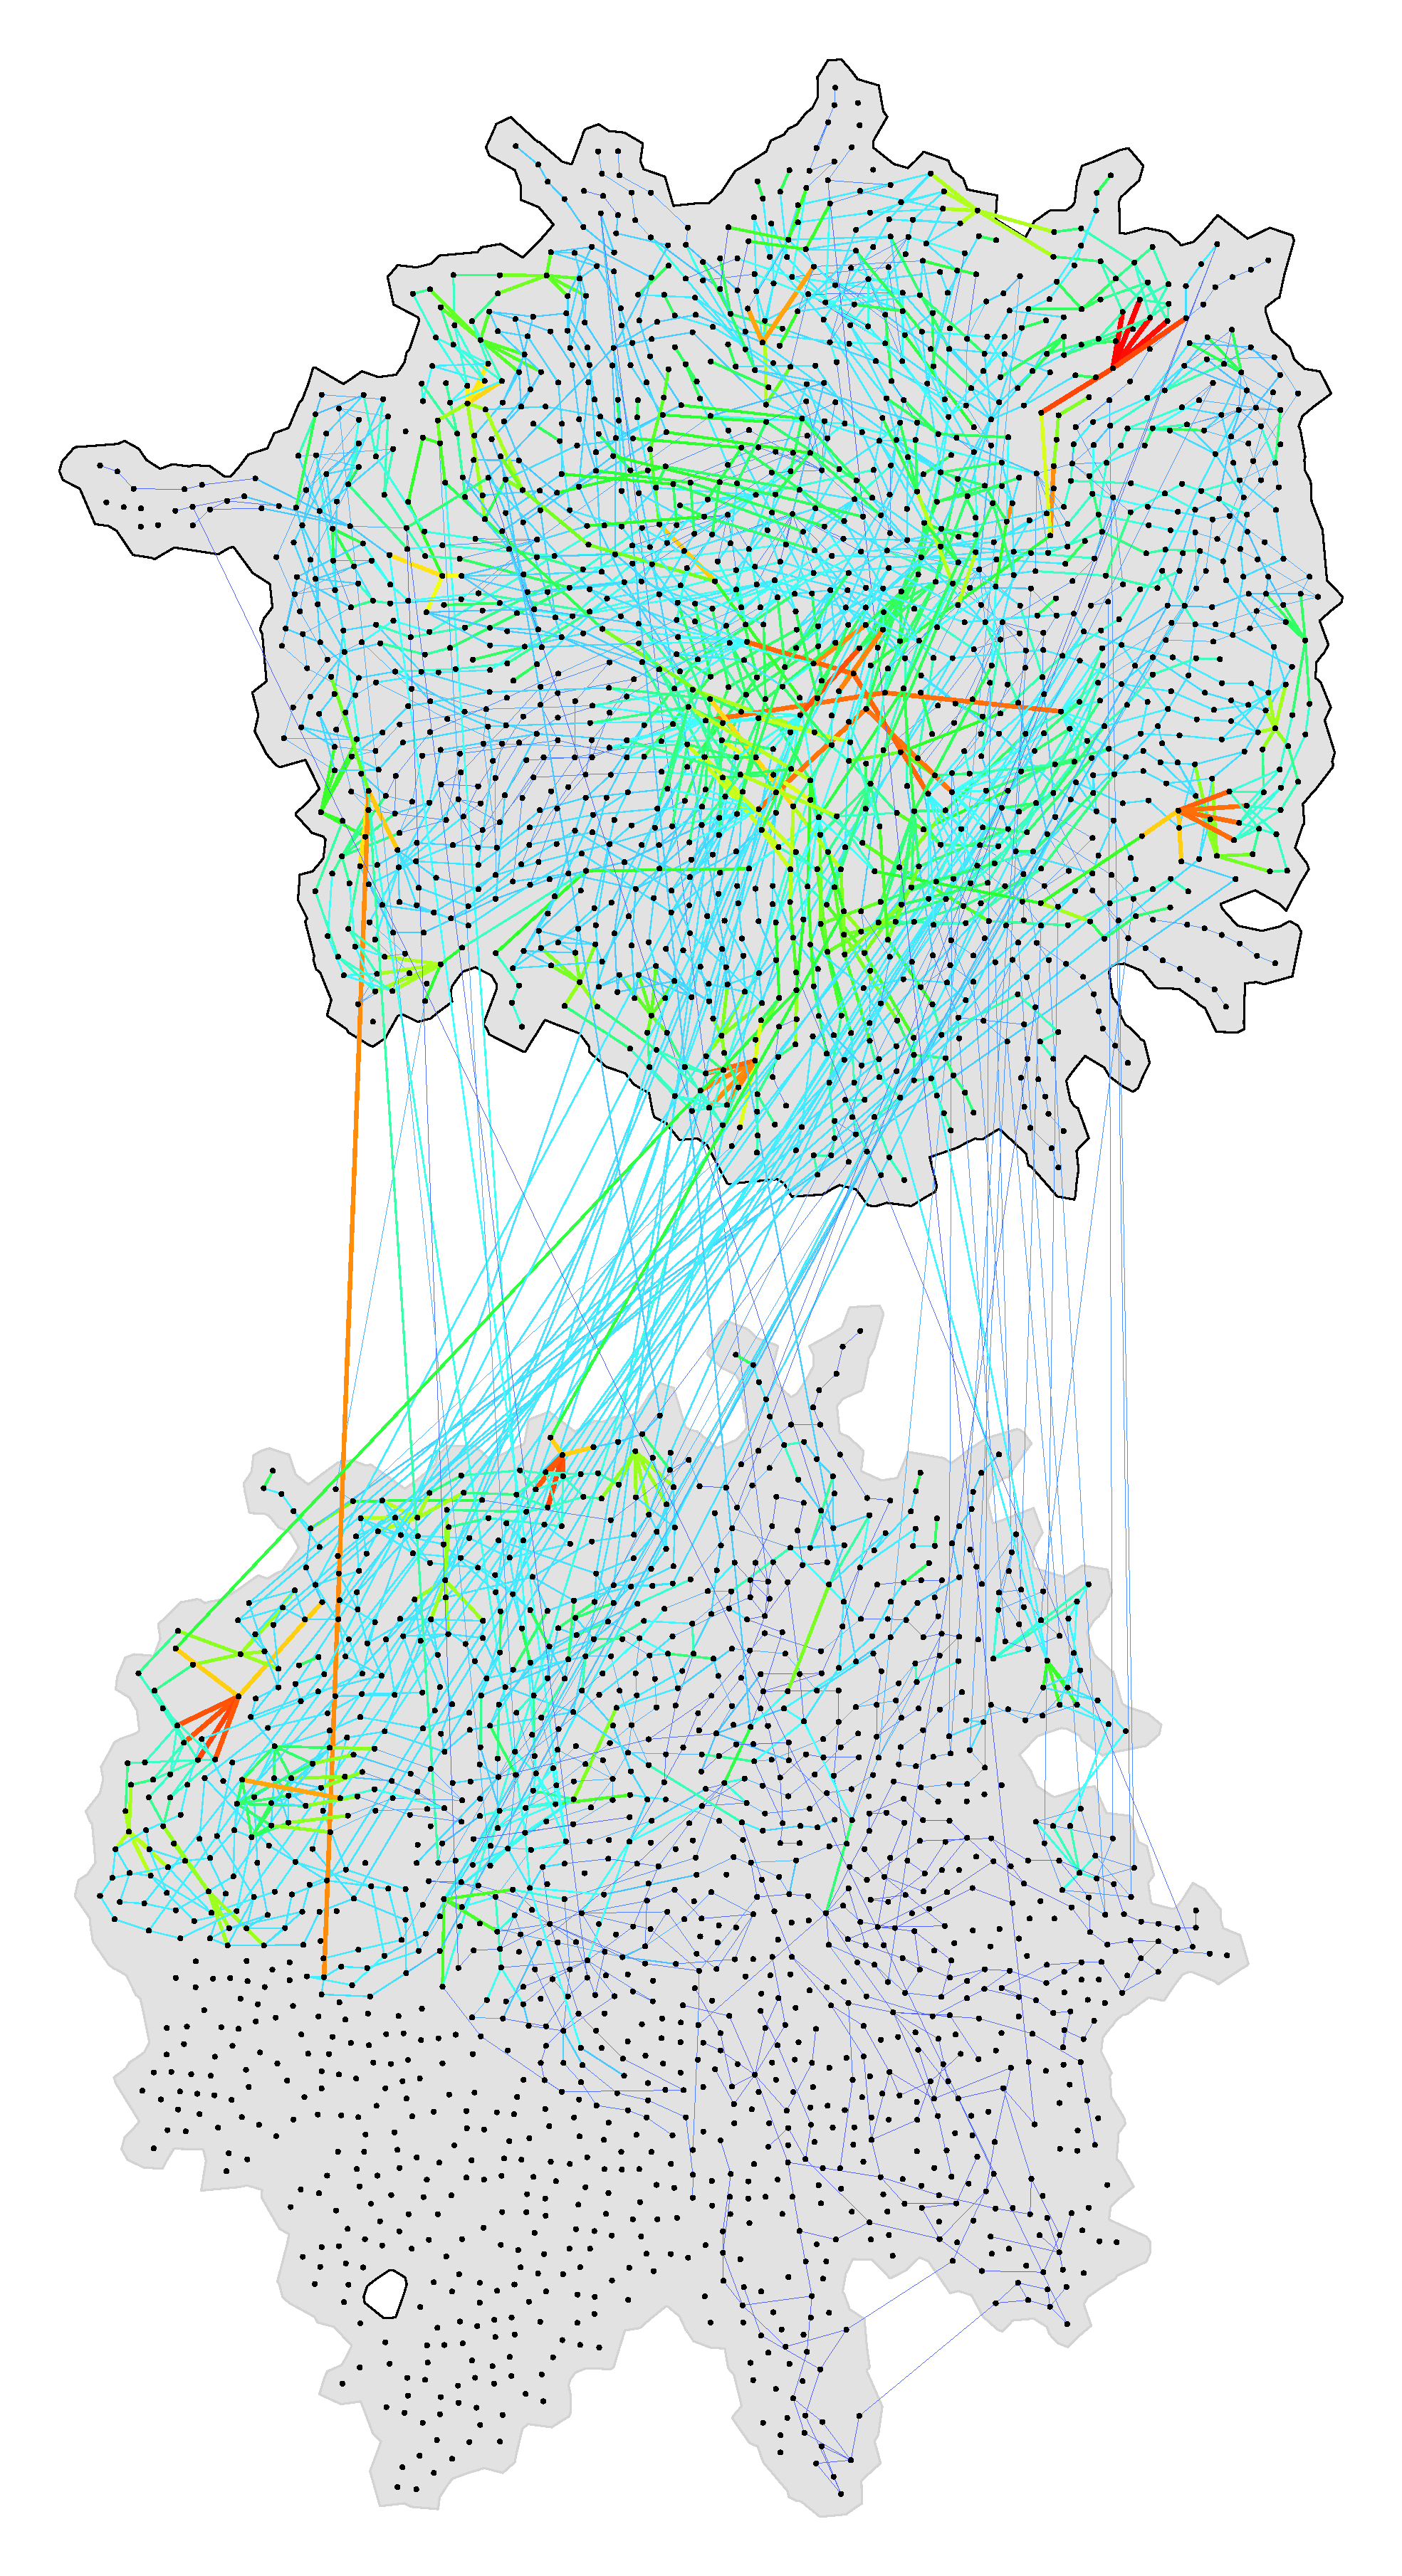
\includegraphics[width=\textwidth,height=0.9\textheight,keepaspectratio]{figs/s5378_2part}
\caption{Heatmap of messages sent during the ISCAS'89 s5378 simulation, partitioned into two partitions using the profile guided algorithm.}
\end{figure}

\begin{figure}
\centering
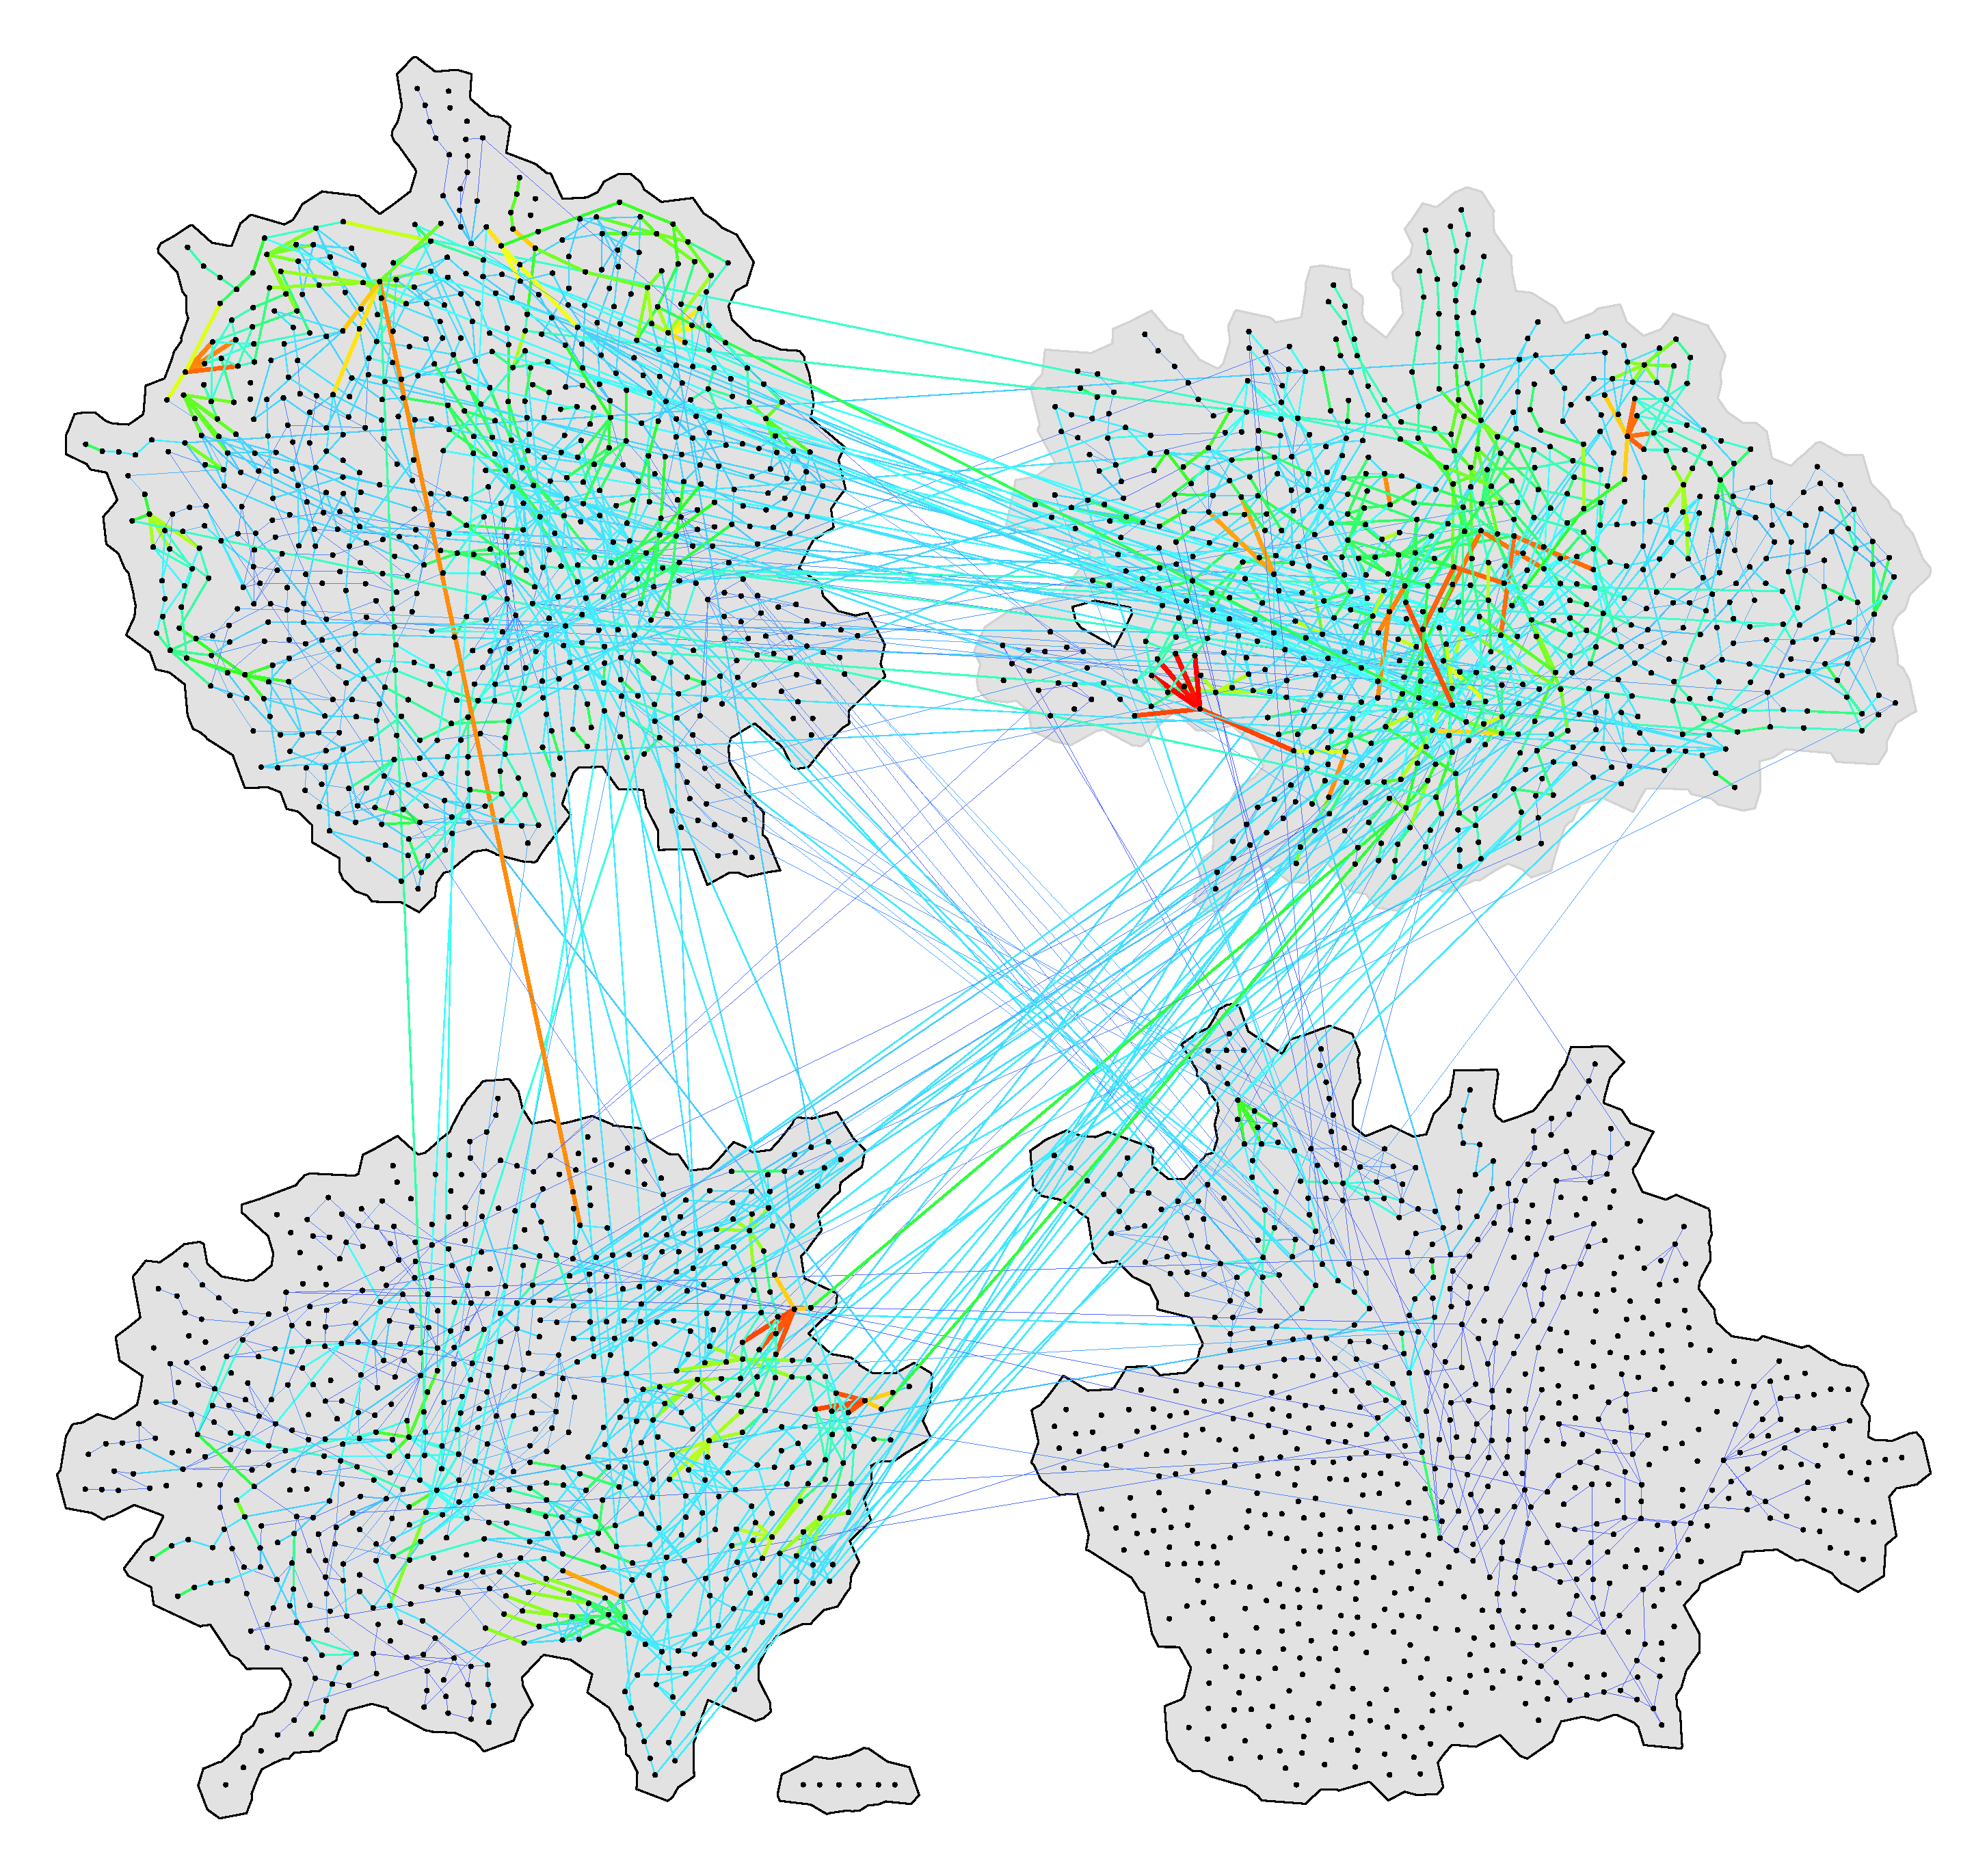
\includegraphics[width=\textwidth,height=0.9\textheight,keepaspectratio]{figs/s5378_4part}
\caption{Heatmap of messages sent during the ISCAS'89 s5378 simulation, partitioned into four partitions using the profile guided algorithm.}
\end{figure}

\begin{figure}
\centering
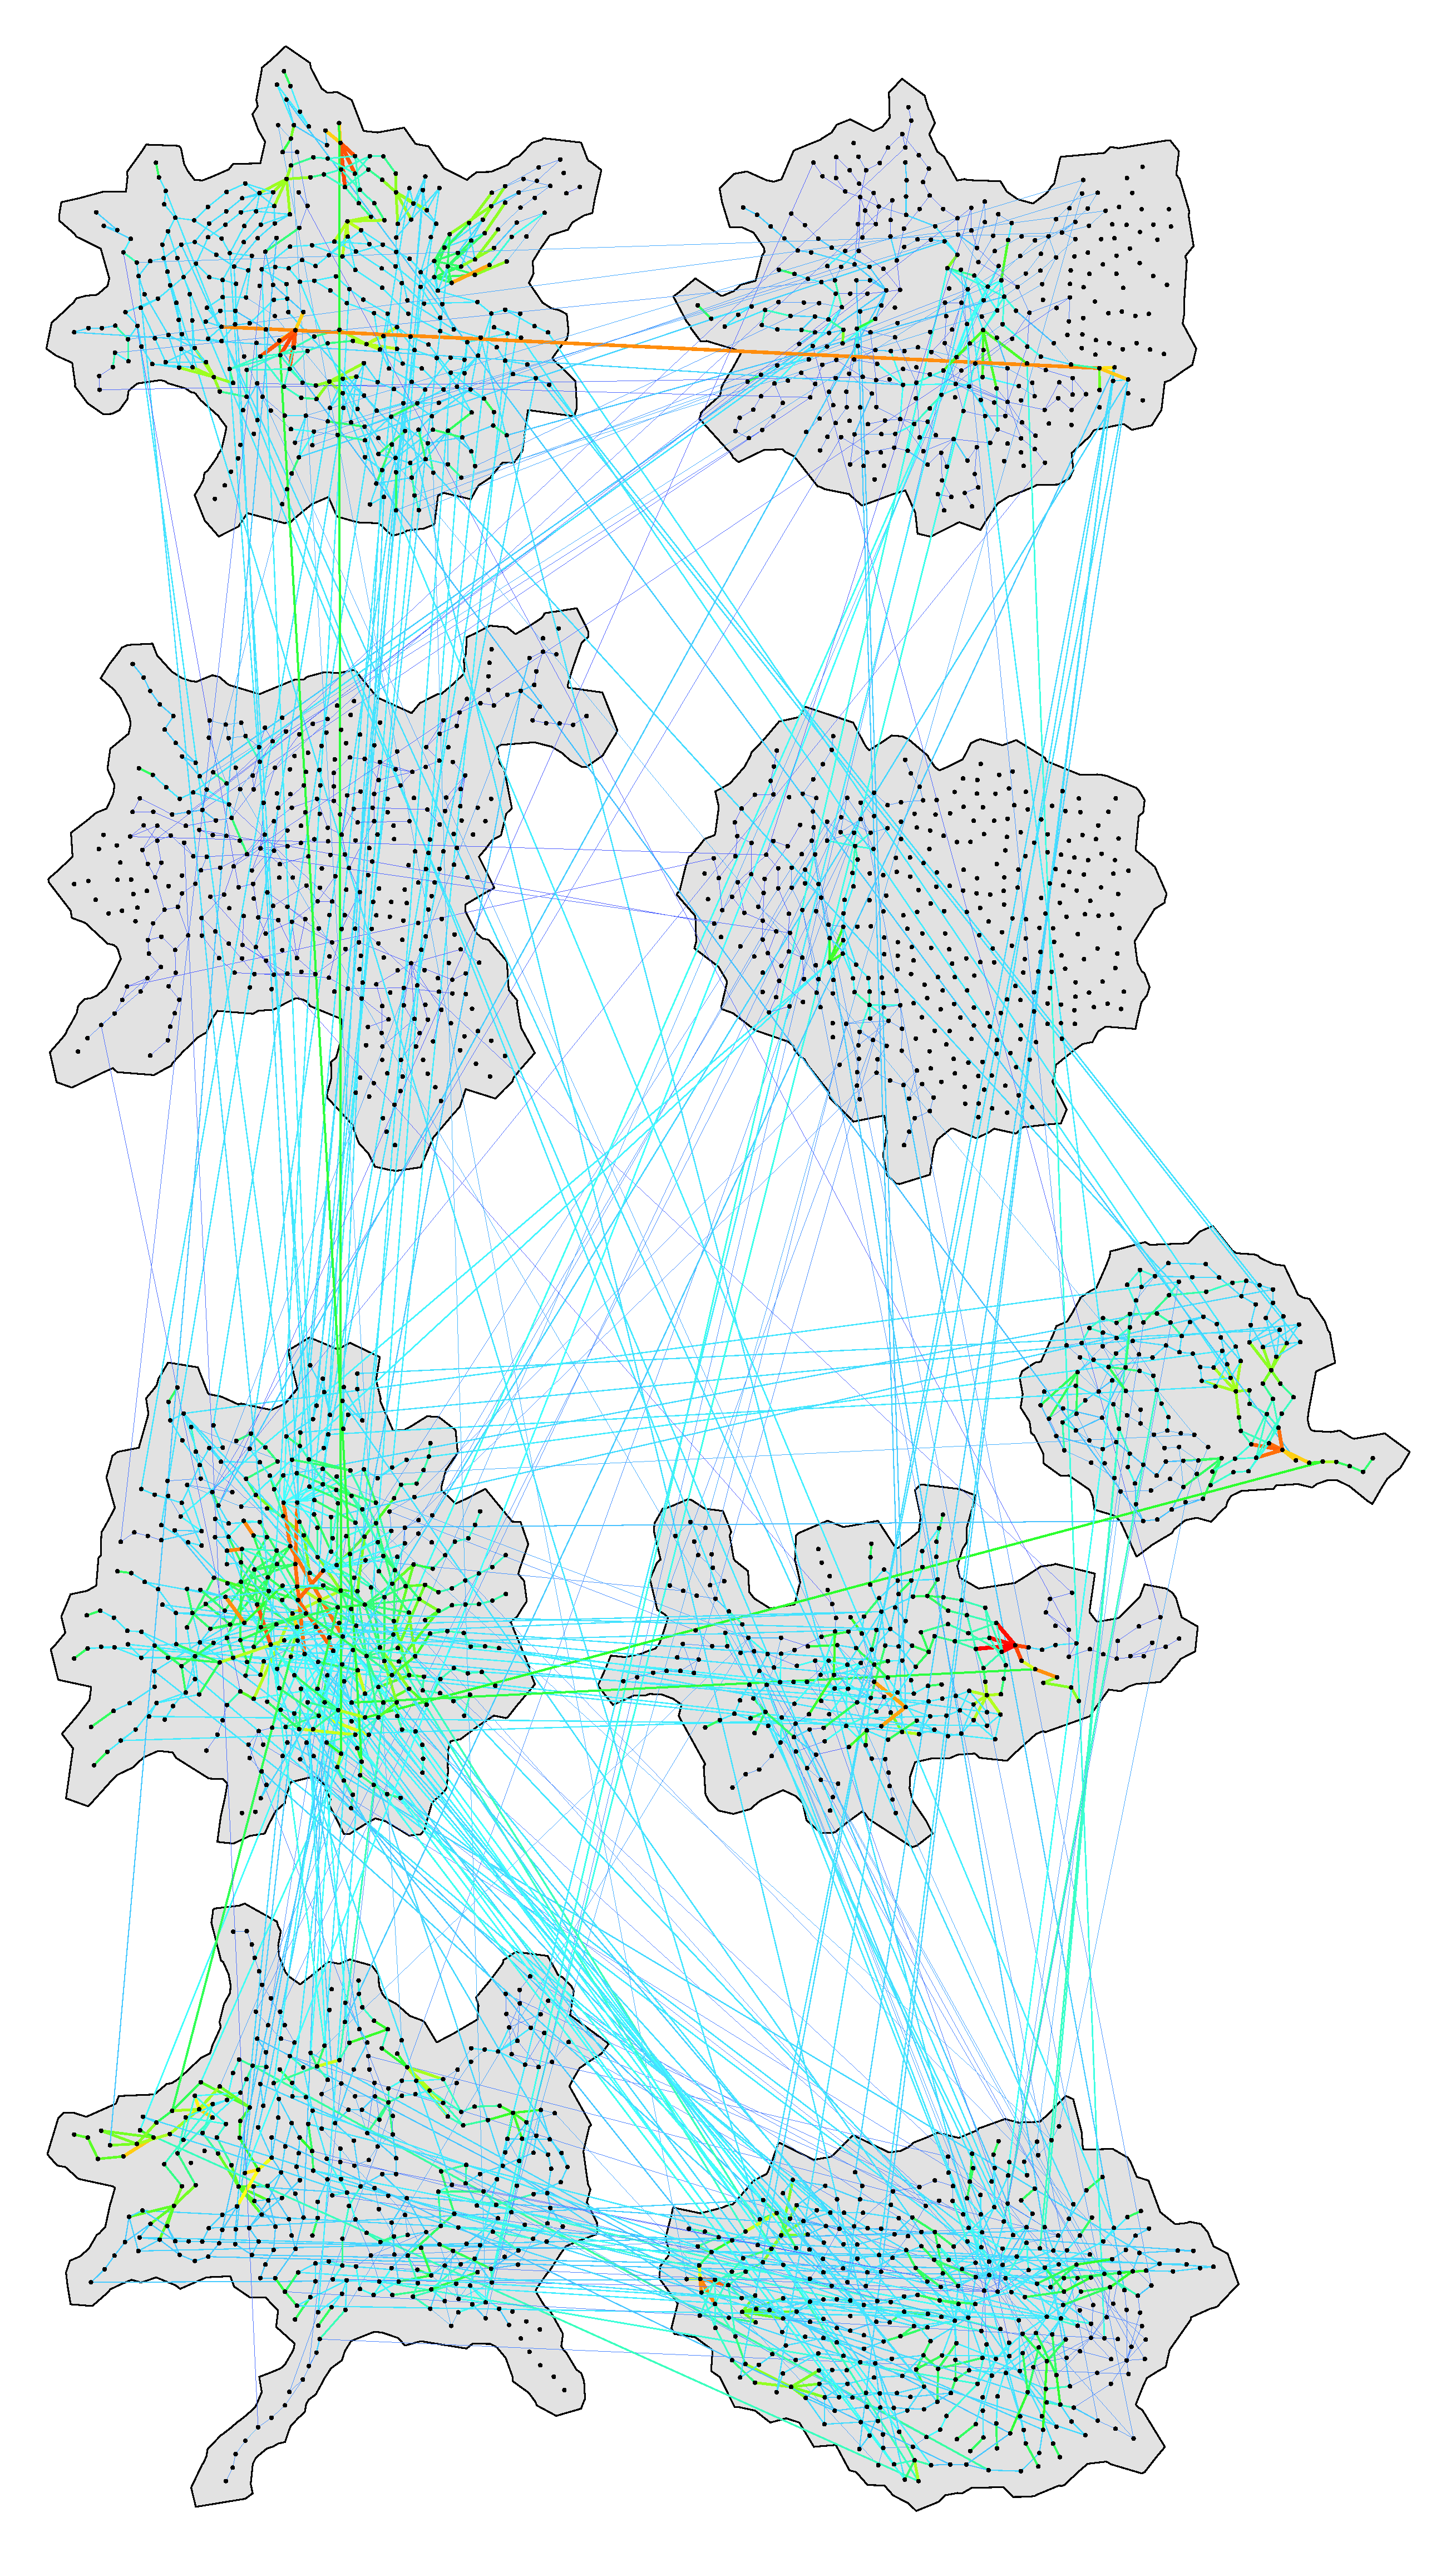
\includegraphics[width=\textwidth,height=0.9\textheight,keepaspectratio]{figs/s5378_8part}
\caption{Heatmap of messages sent during the ISCAS'89 s5378 simulation, partitioned into eight partitions using the profile guided algorithm.}
\end{figure}

\begin{figure}
\centering
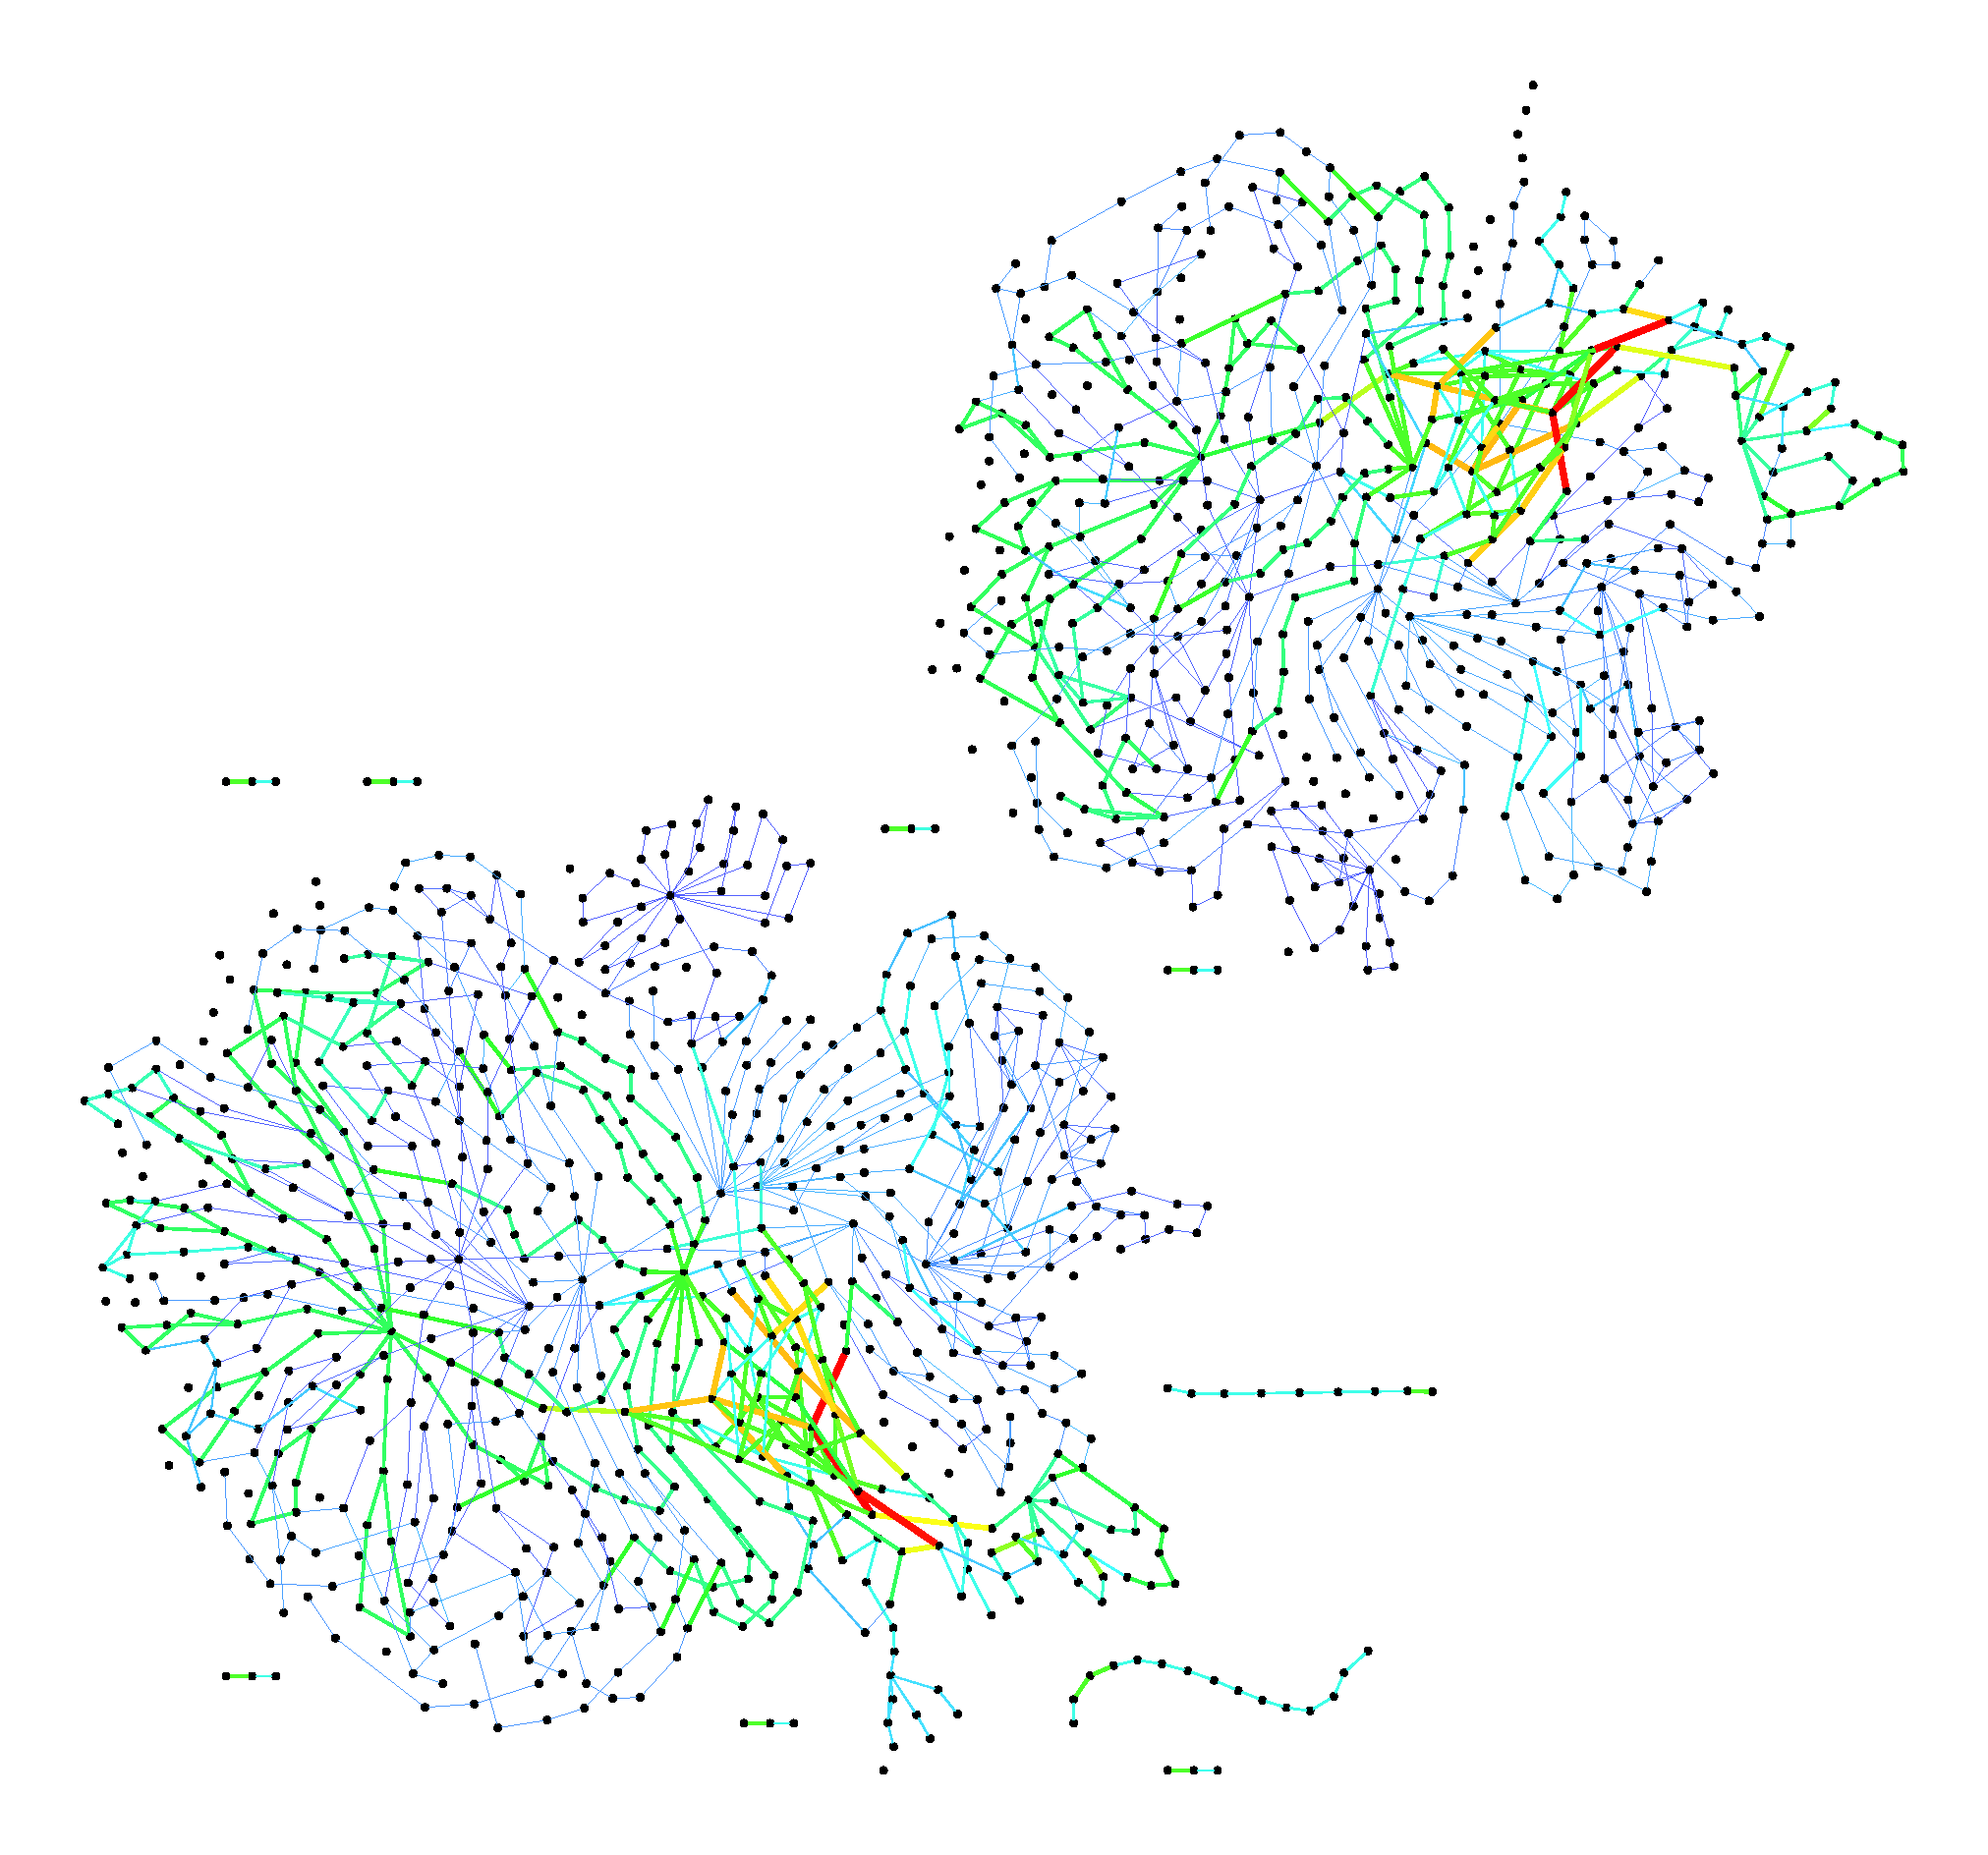
\includegraphics[width=\textwidth,height=0.9\textheight,keepaspectratio]{figs/s9234}
\caption{Heatmap of messages sent during the ISCAS'89 s9234 simulation.}
\end{figure}

\begin{figure}
\centering
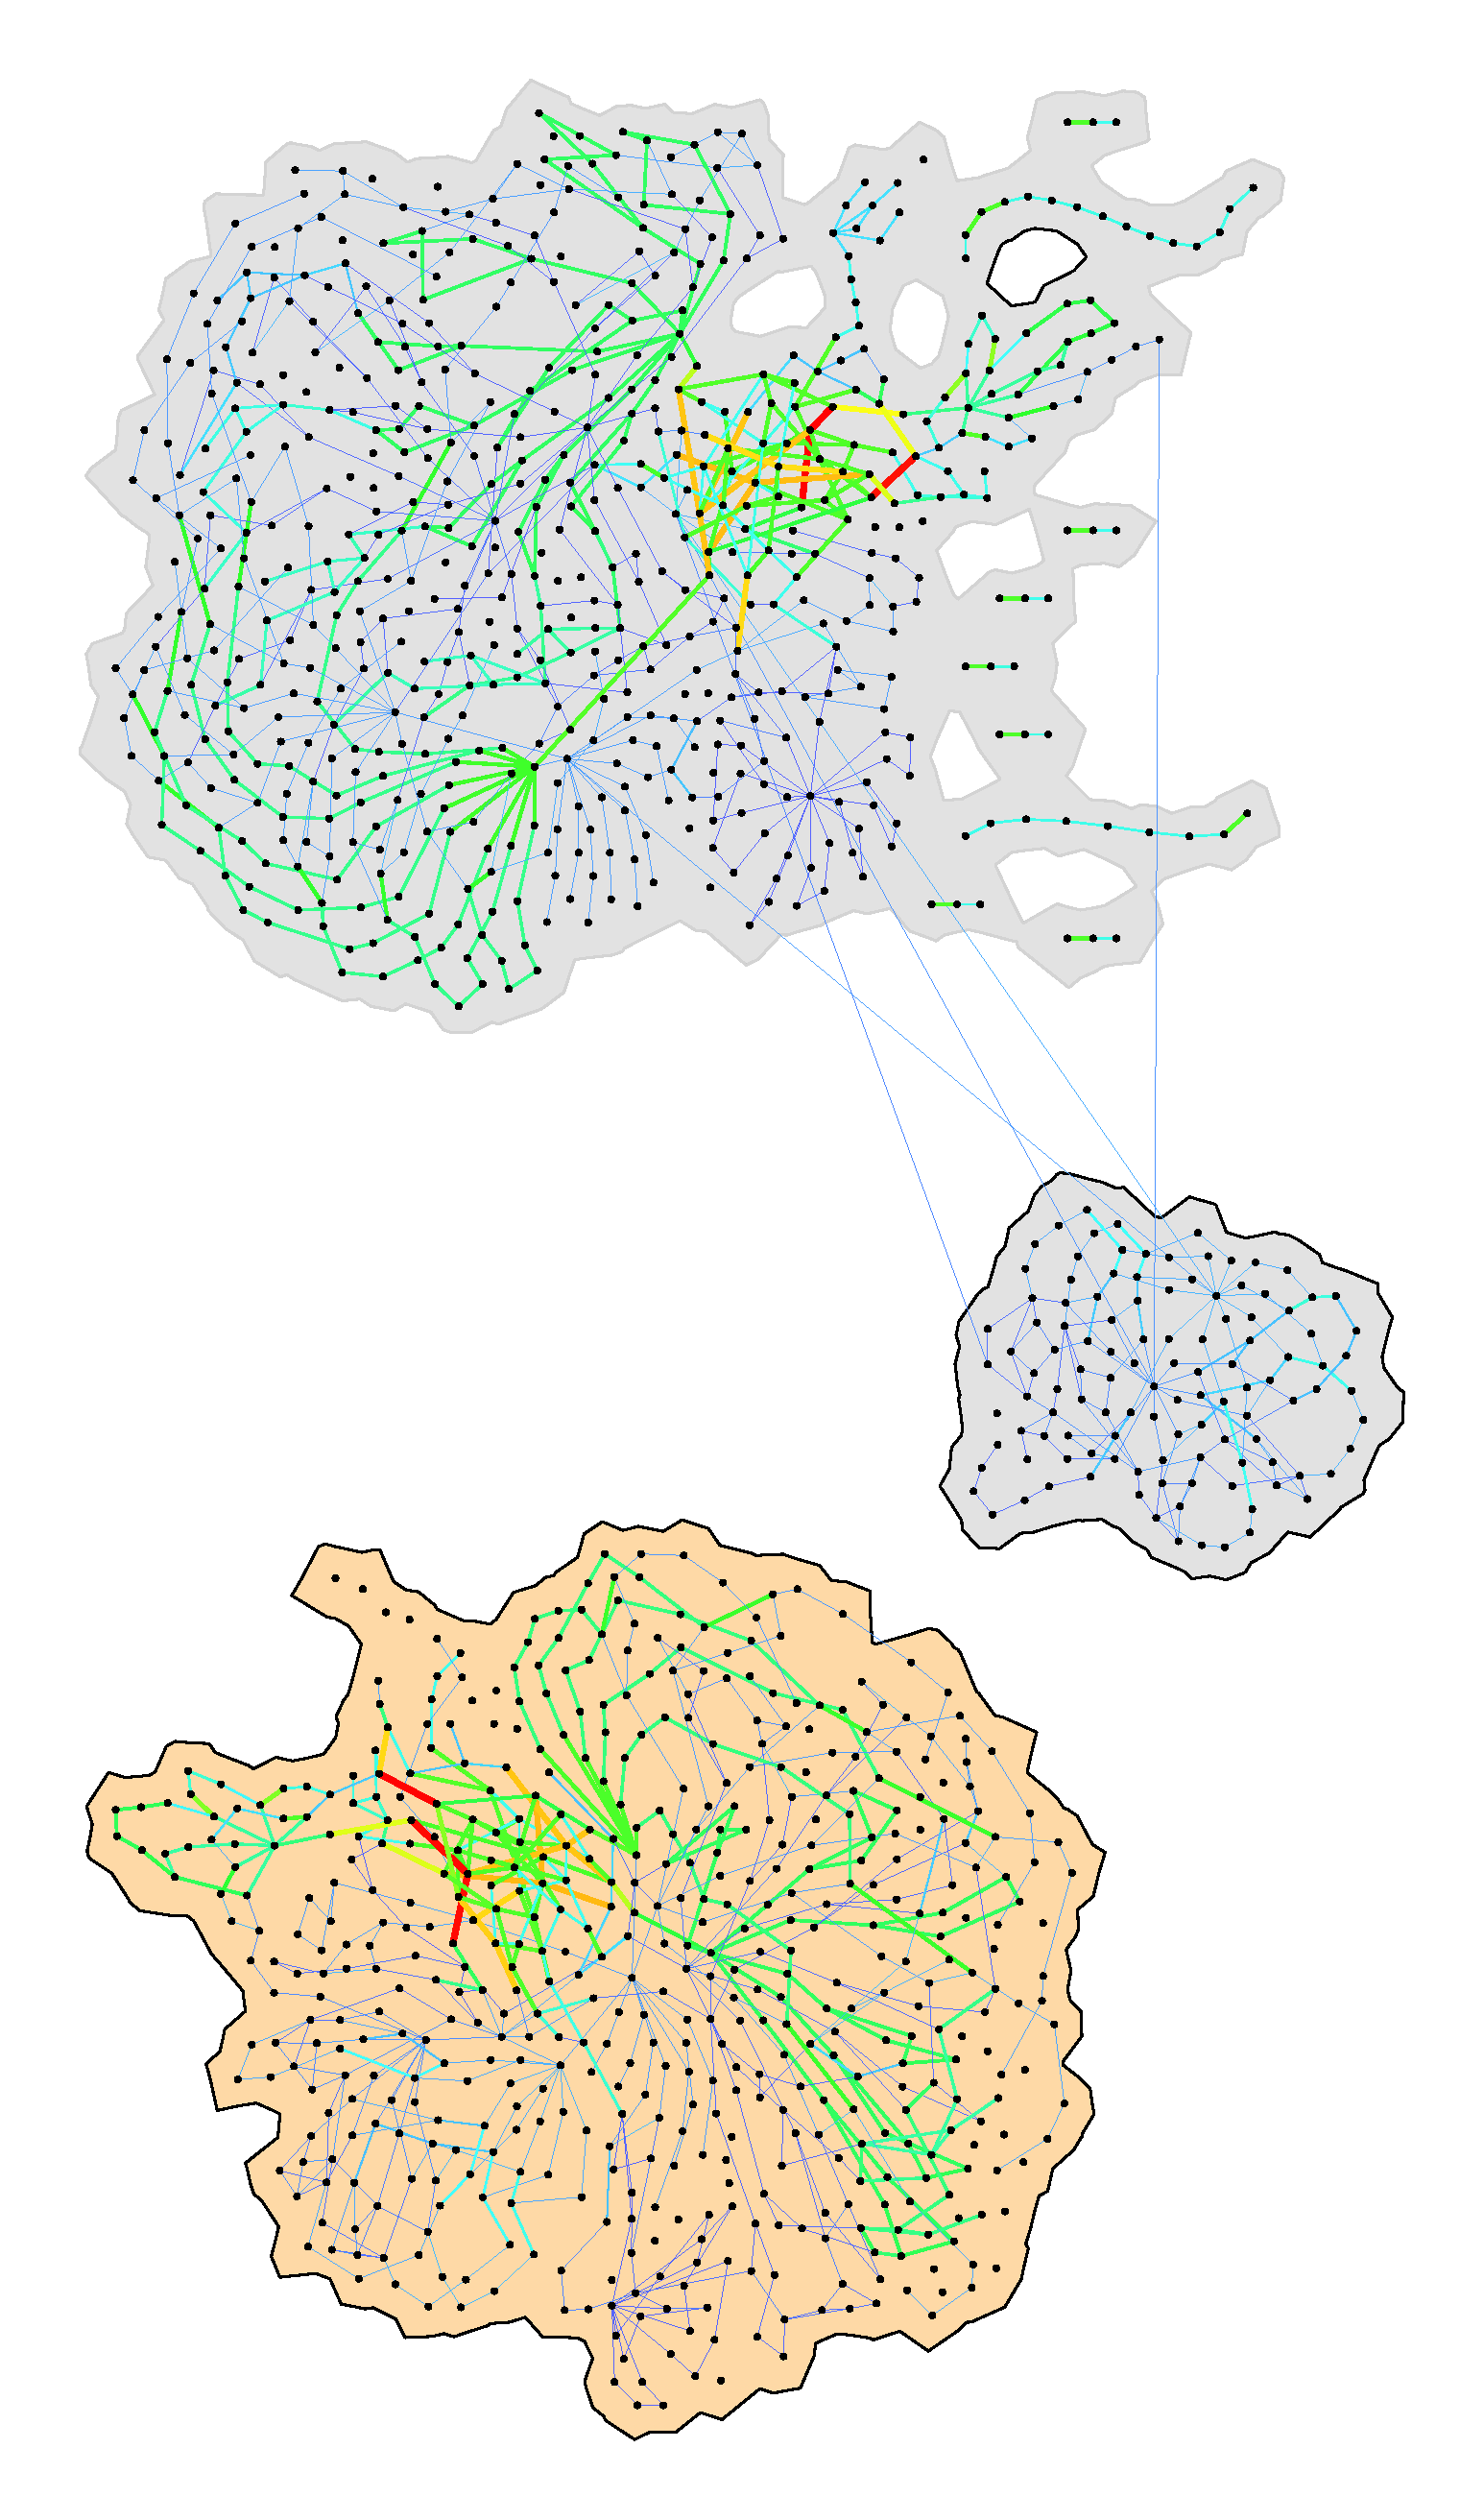
\includegraphics[width=\textwidth,height=0.9\textheight,keepaspectratio]{figs/s9234_2part}
\caption{Heatmap of messages sent during the ISCAS'89 s9234 simulation, partitioned into two partitions using the profile guided algorithm.}
\end{figure}

\begin{figure}
\centering
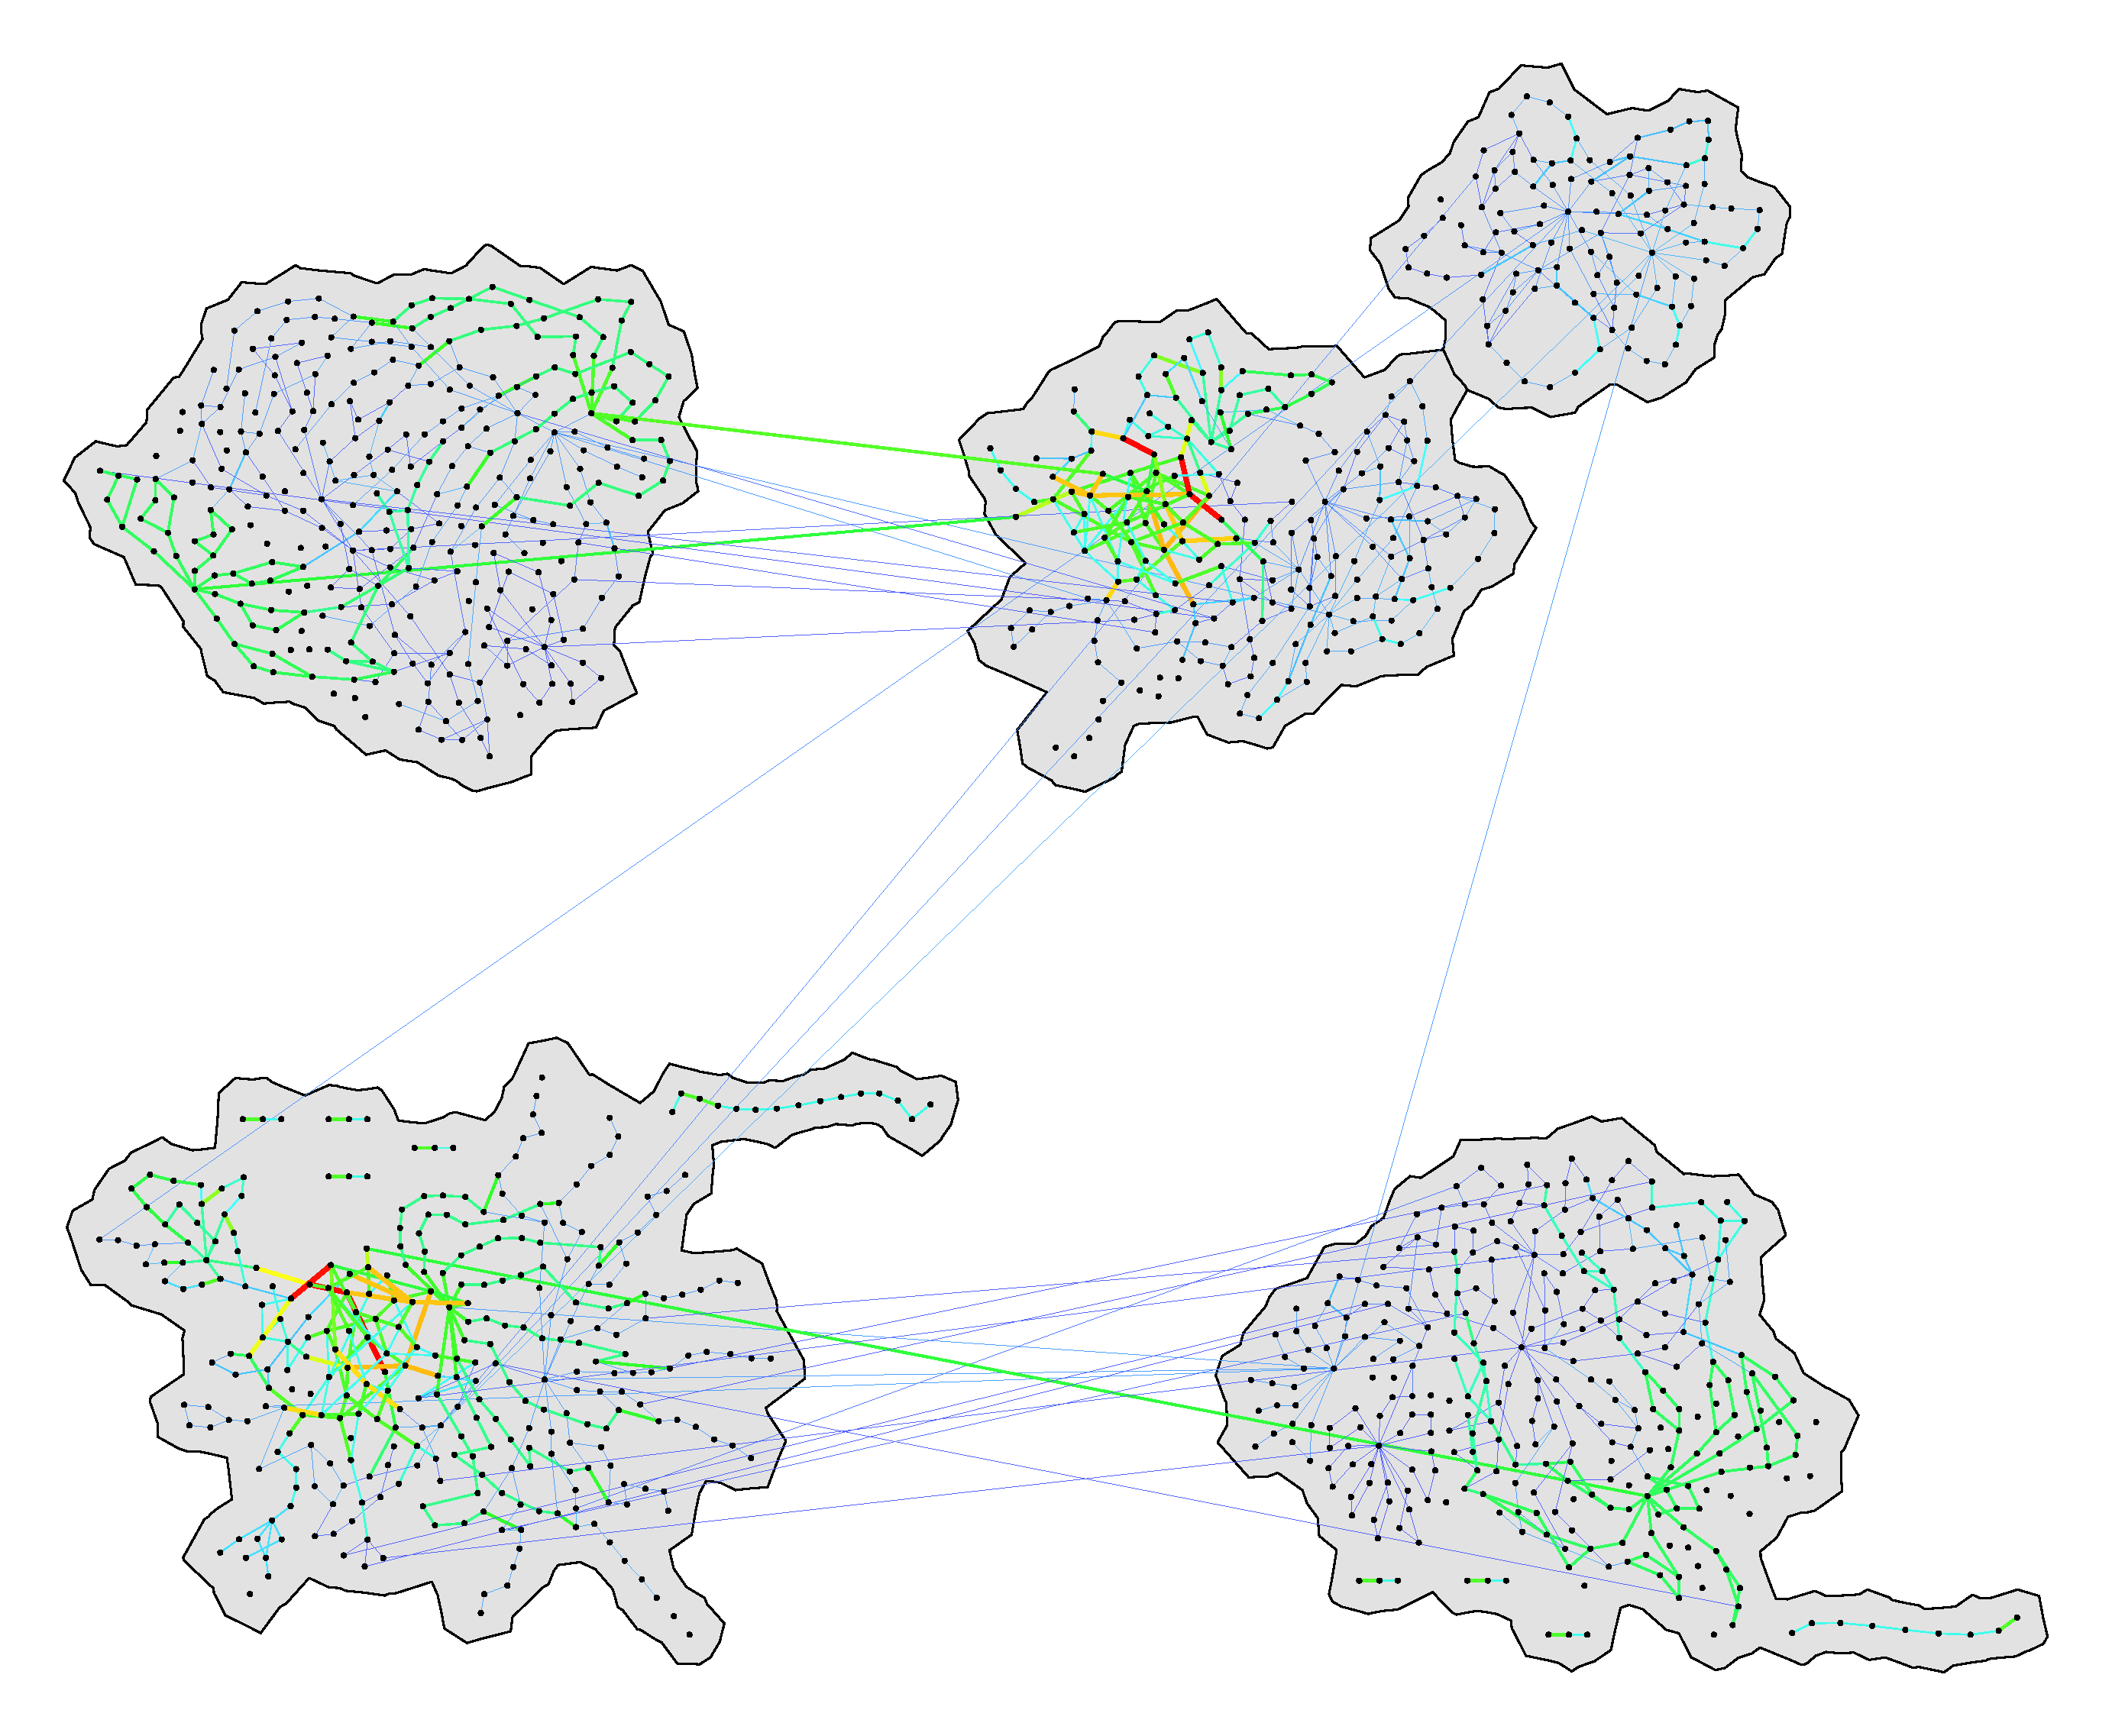
\includegraphics[width=\textwidth,height=0.9\textheight,keepaspectratio]{figs/s9234_4part}
\caption{Heatmap of messages sent during the ISCAS'89 s9234 simulation, partitioned into four partitions using the profile guided algorithm.}
\end{figure}

\begin{figure}
\centering
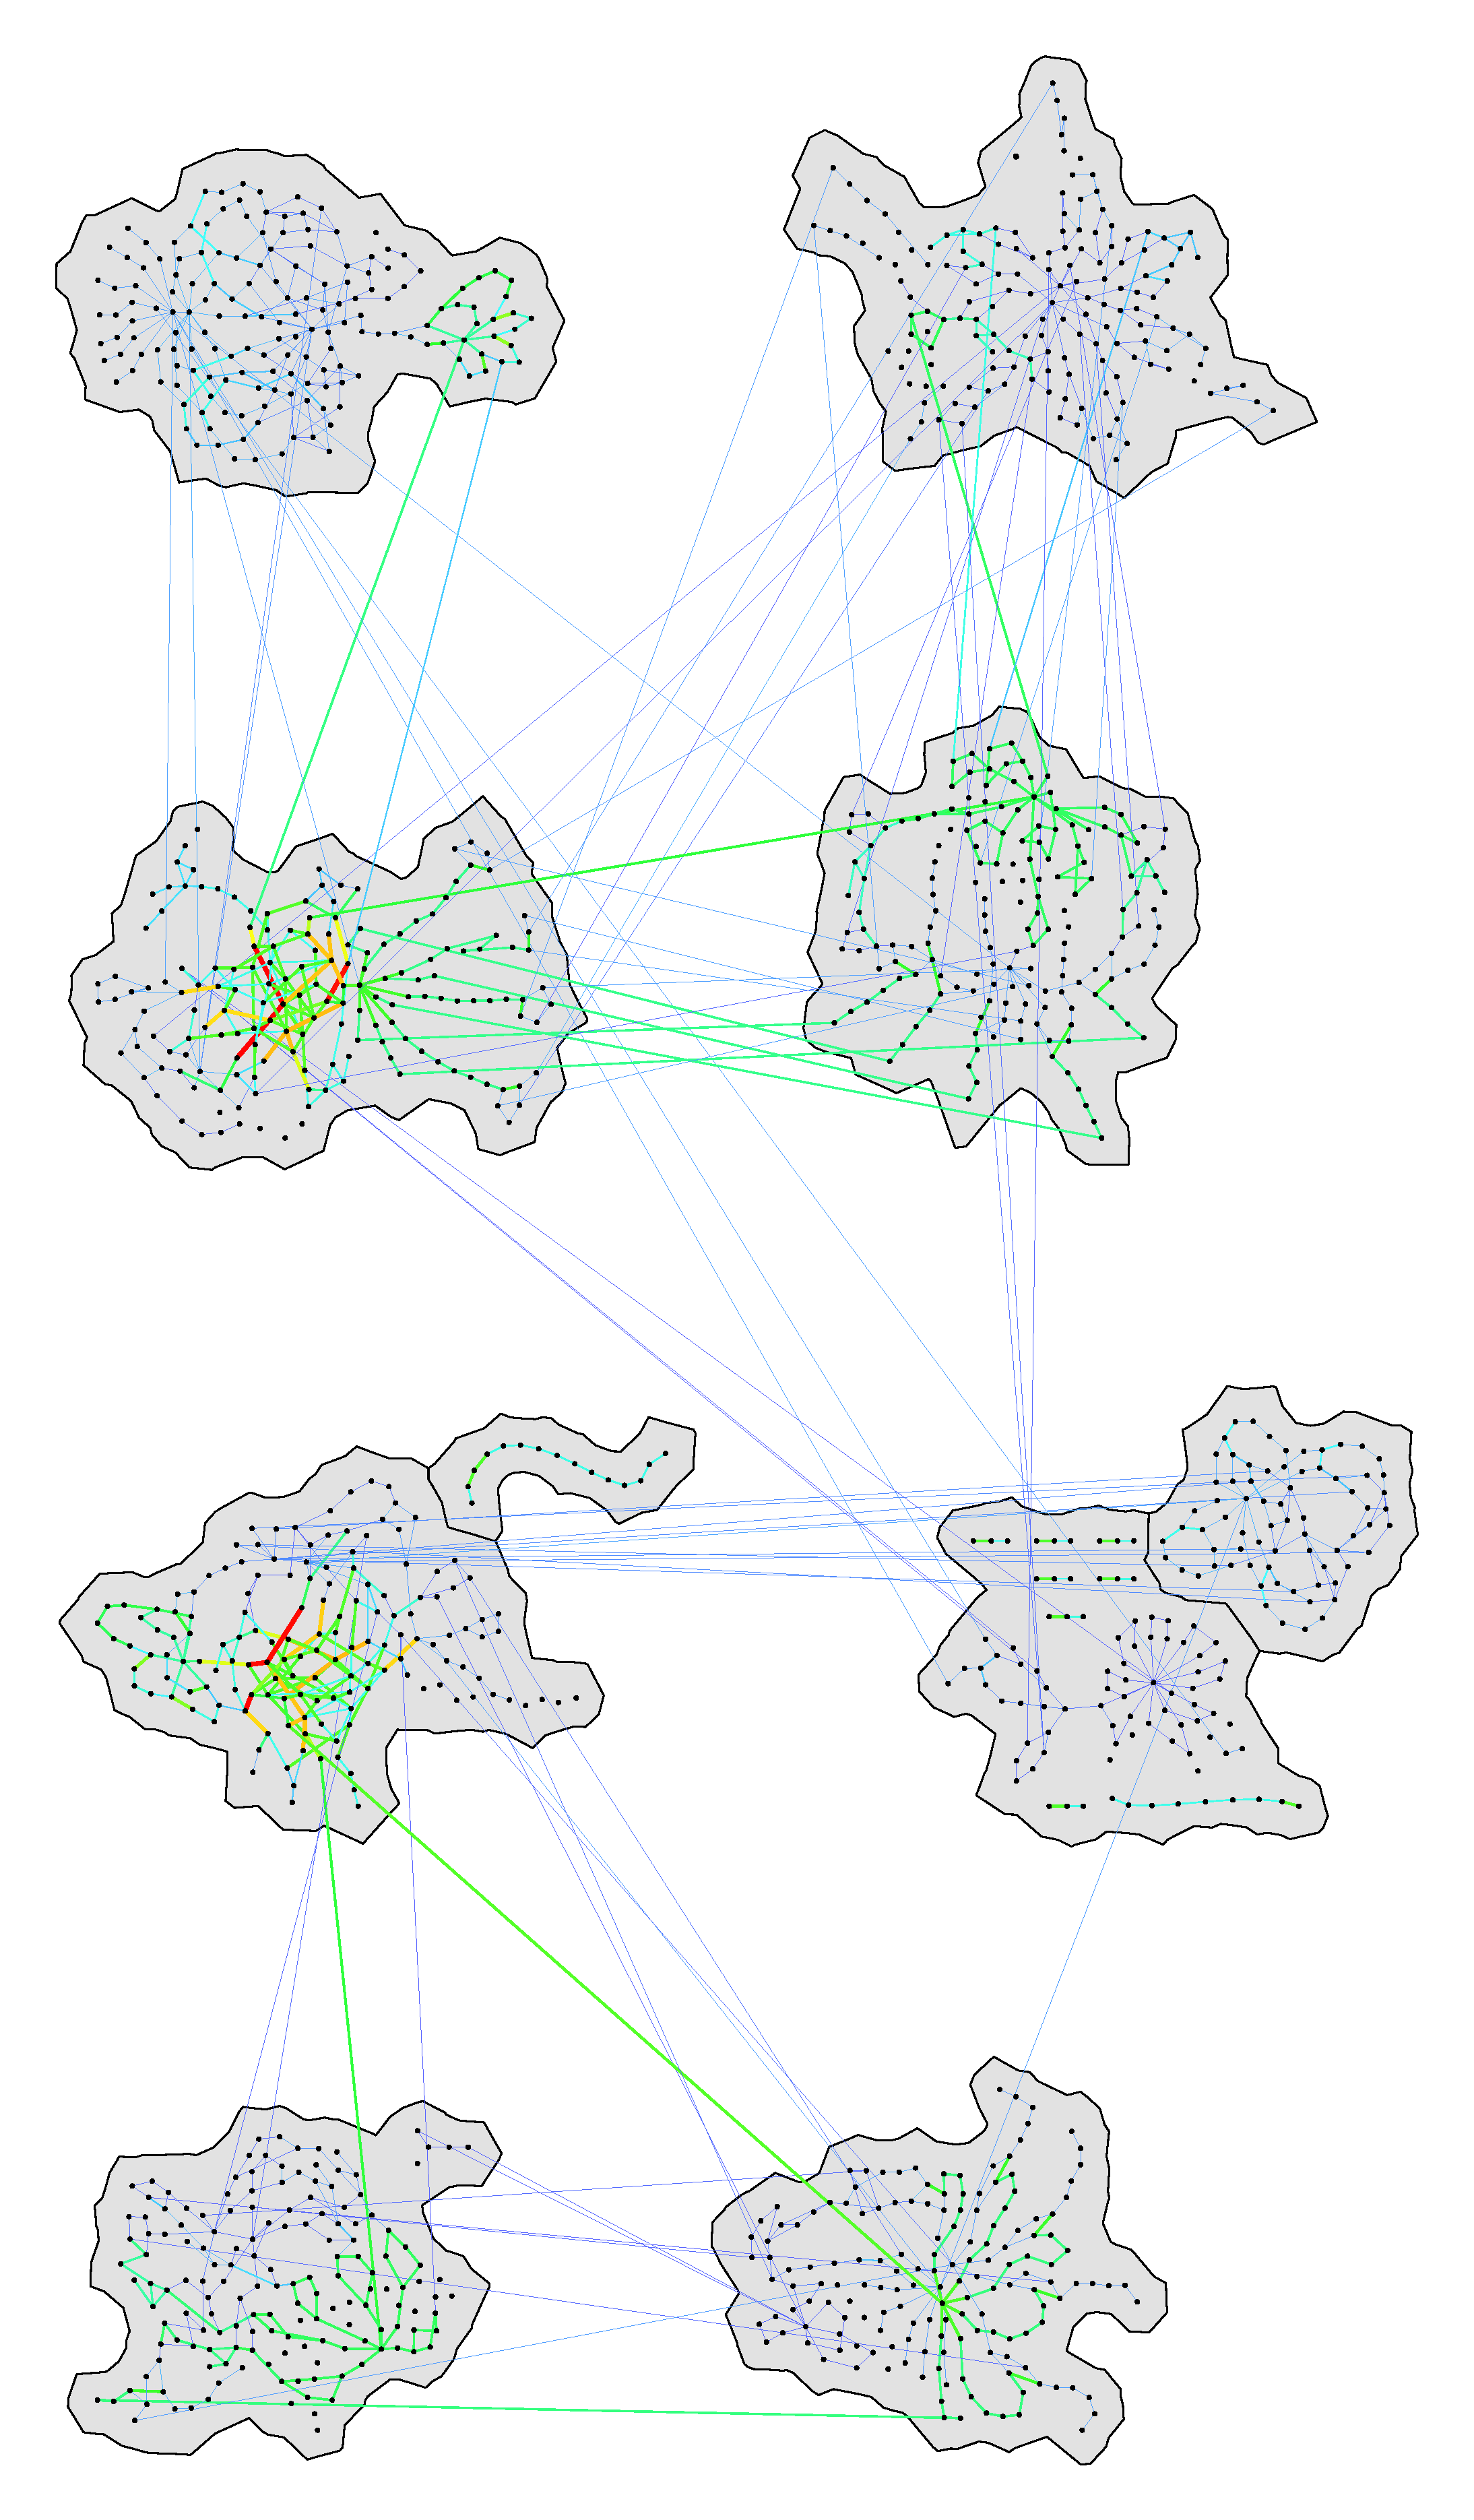
\includegraphics[width=\textwidth,height=0.9\textheight,keepaspectratio]{figs/s9234_8part}
\caption{Heatmap of messages sent during the ISCAS'89 s9234 simulation, partitioned into eight partitions using the profile guided algorithm.}
\end{figure}

\begin{figure}
\centering
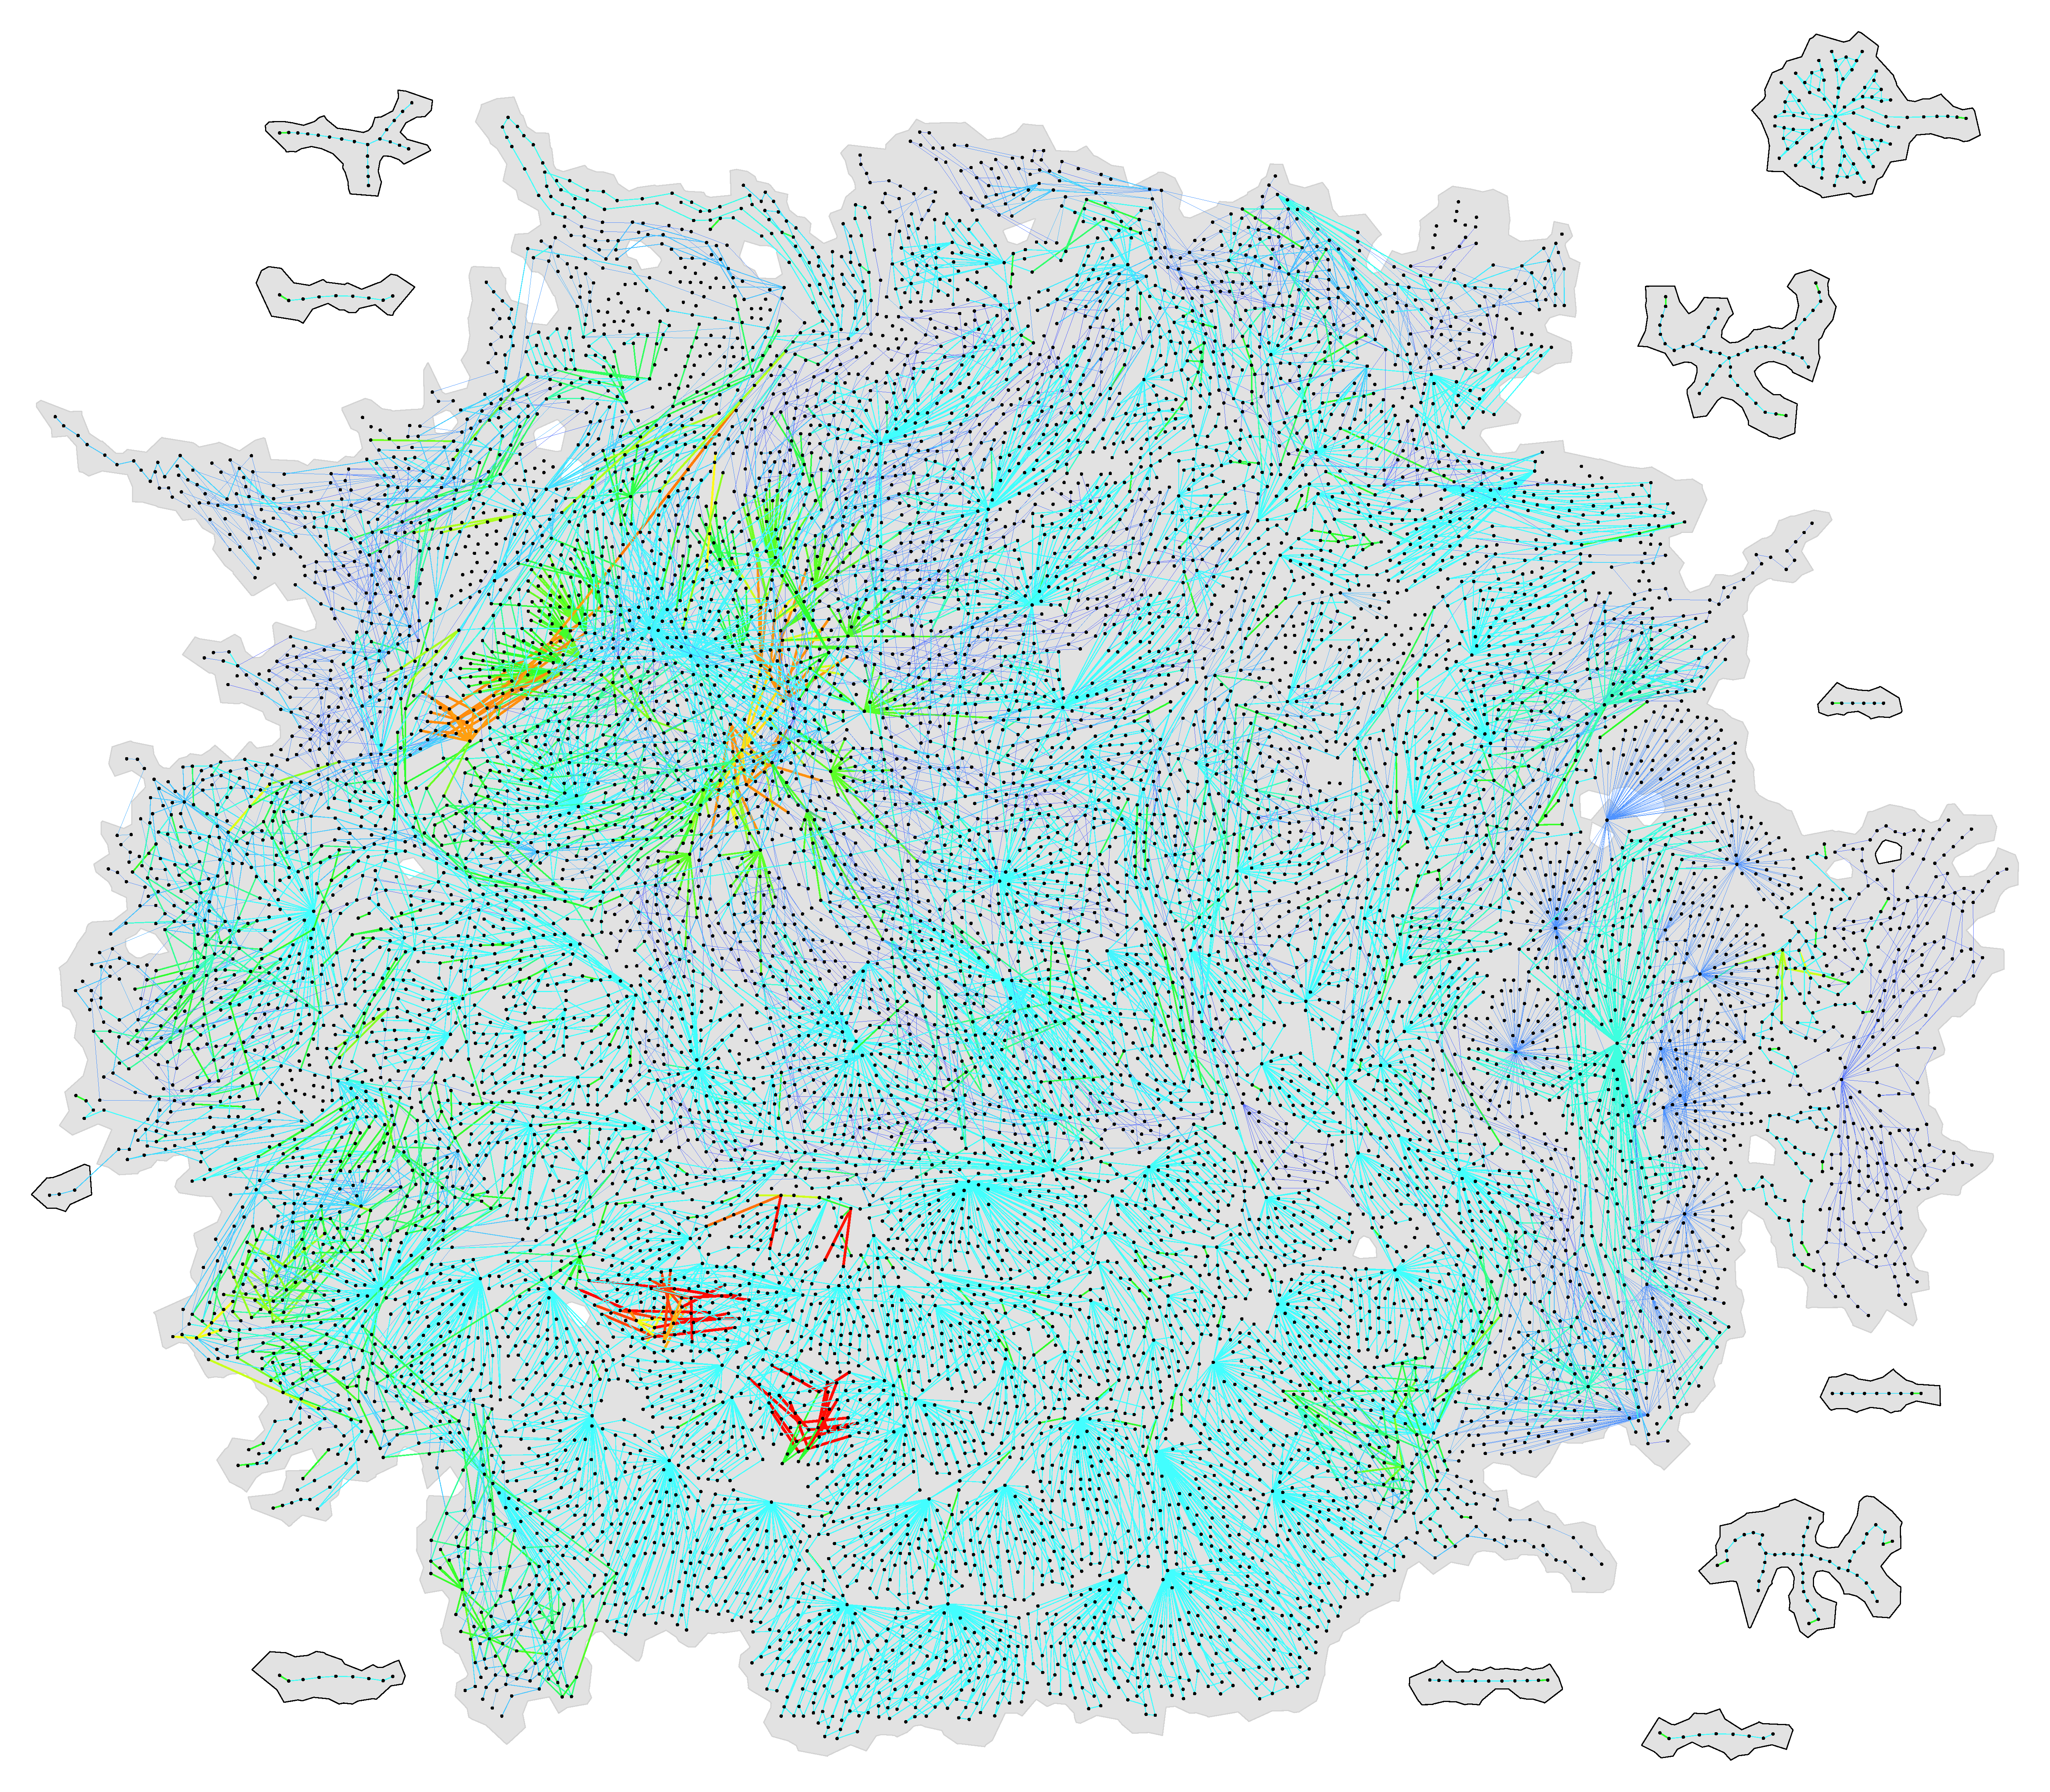
\includegraphics[width=\textwidth,height=0.9\textheight,keepaspectratio]{figs/s38584}
\caption{Heatmap of messages sent during the ISCAS'89 s38584 simulation.}
\end{figure}

\begin{figure}
\centering
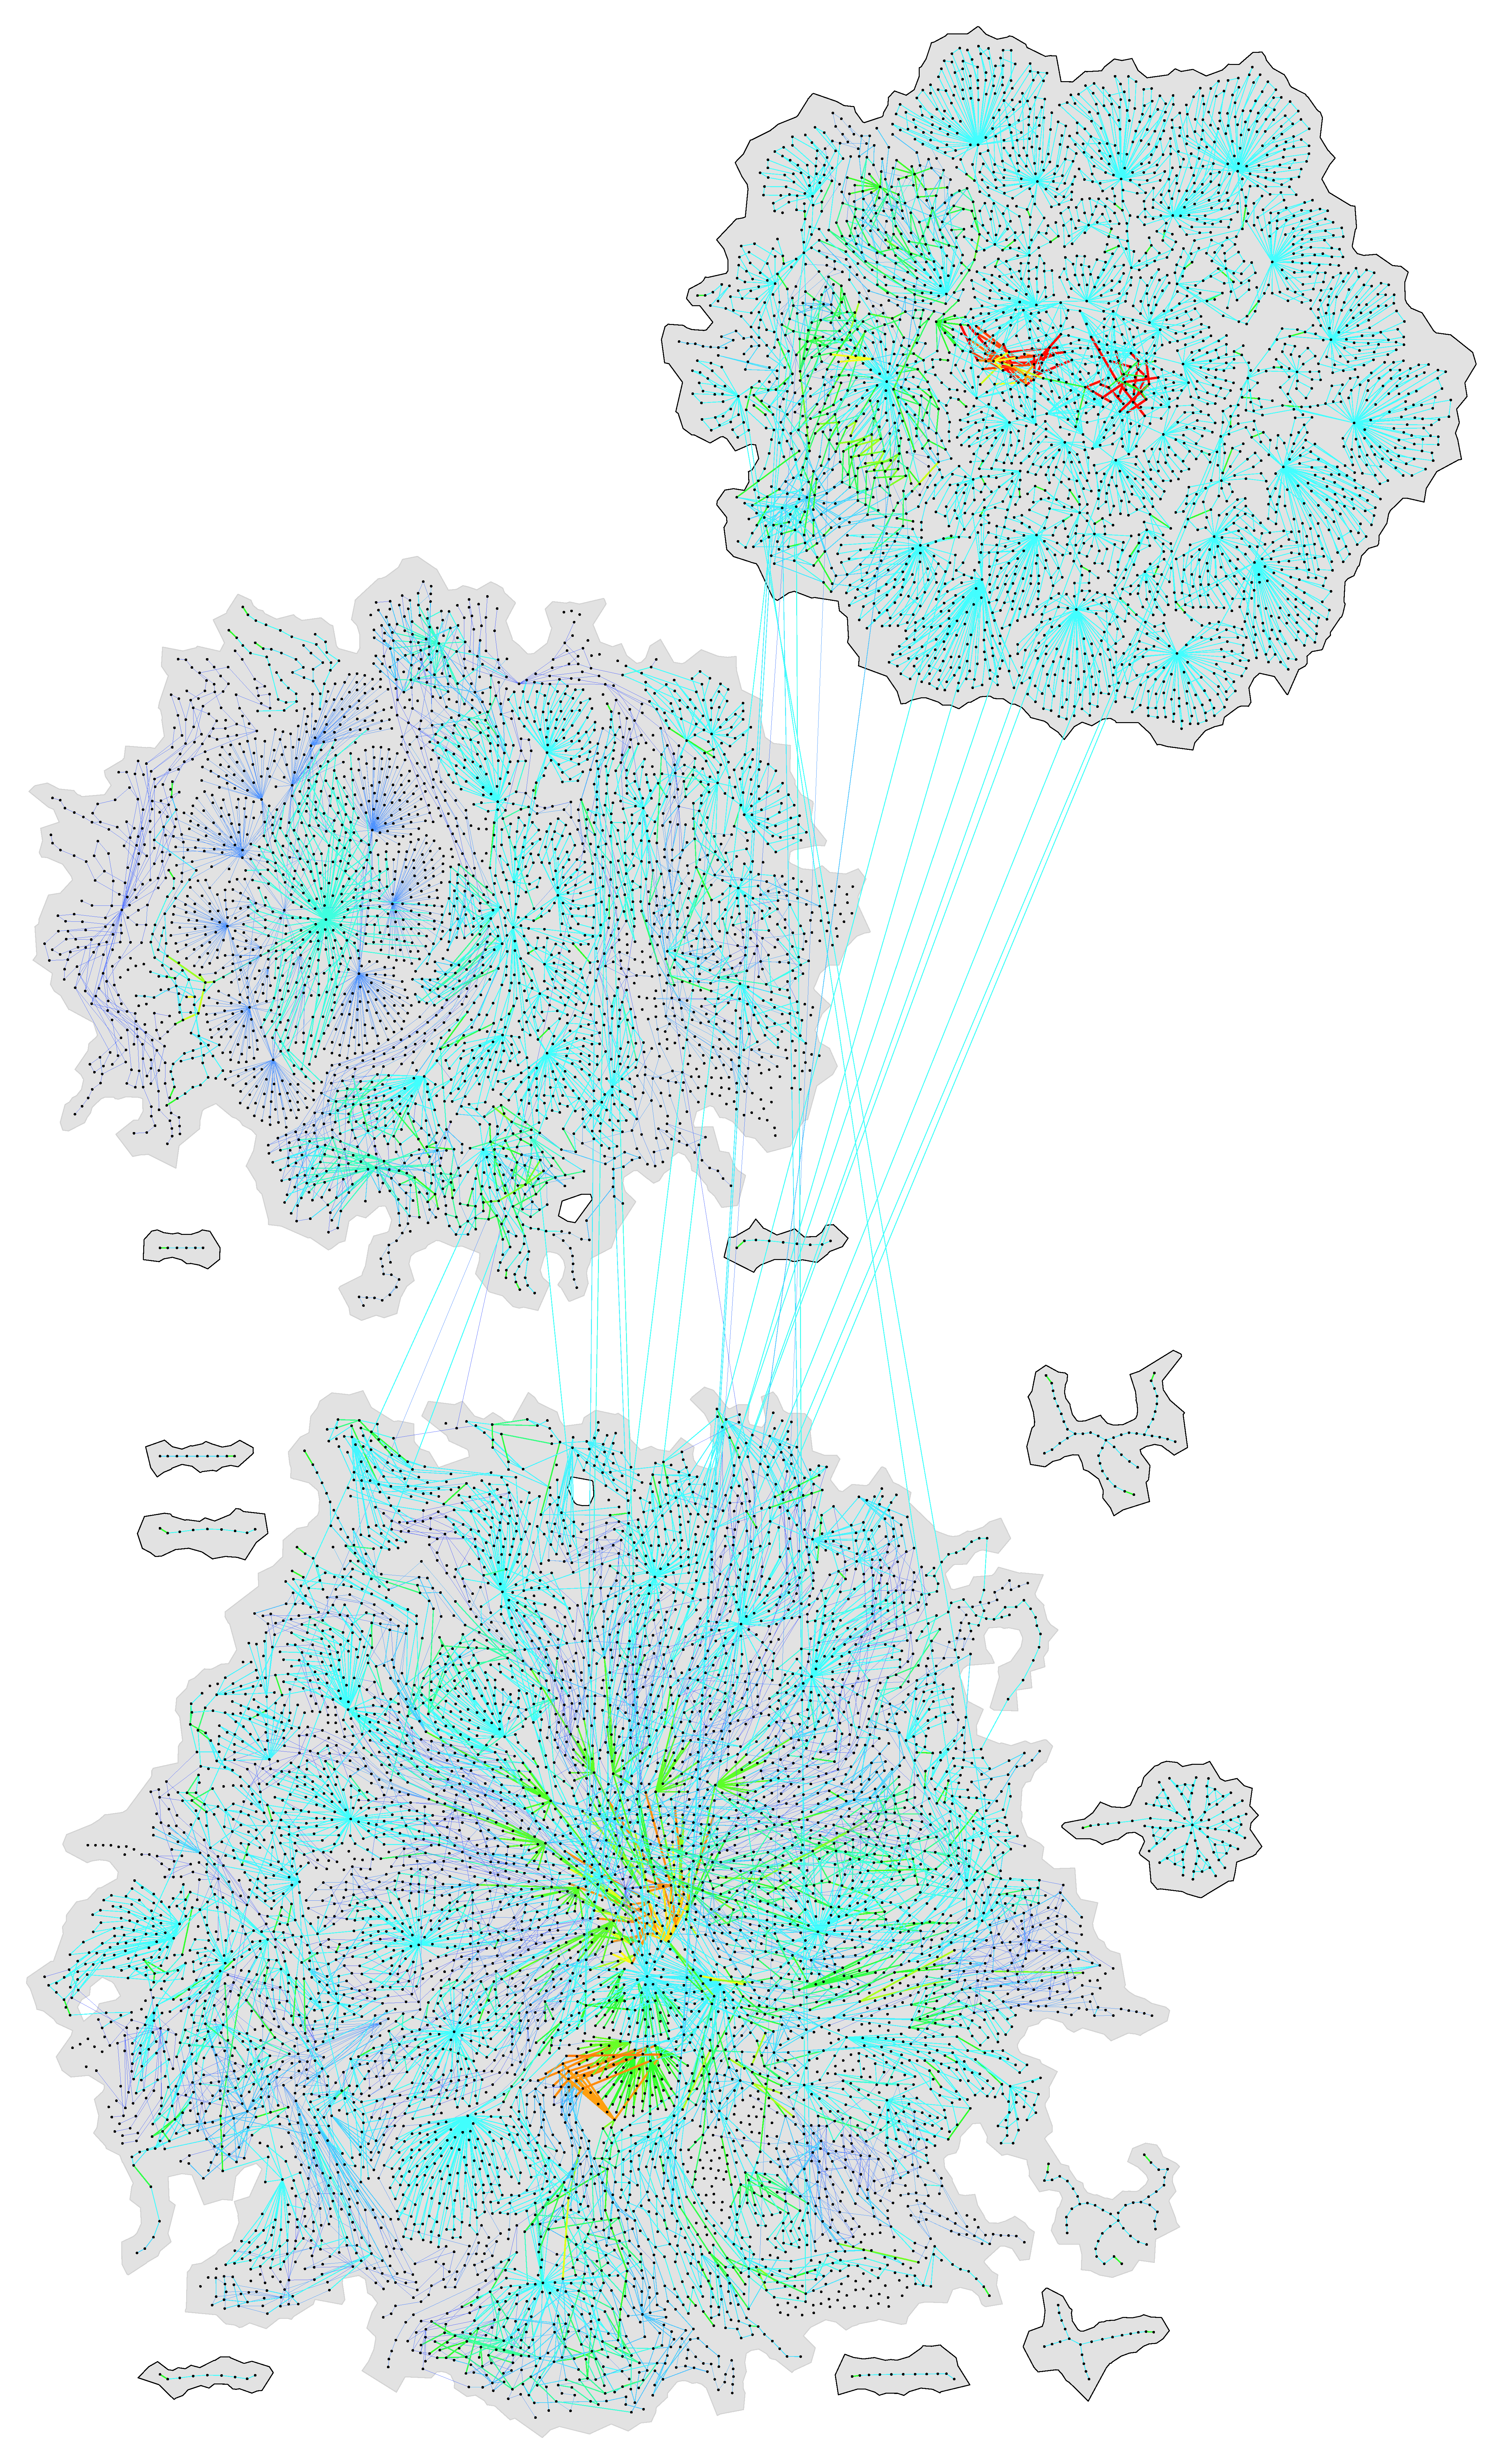
\includegraphics[width=\textwidth,height=0.9\textheight,keepaspectratio]{figs/s38584_2part}
\caption{Heatmap of messages sent during the ISCAS'89 s38584 simulation, partitioned into two partitions using the profile guided algorithm.}
\end{figure}

\begin{figure}
\centering
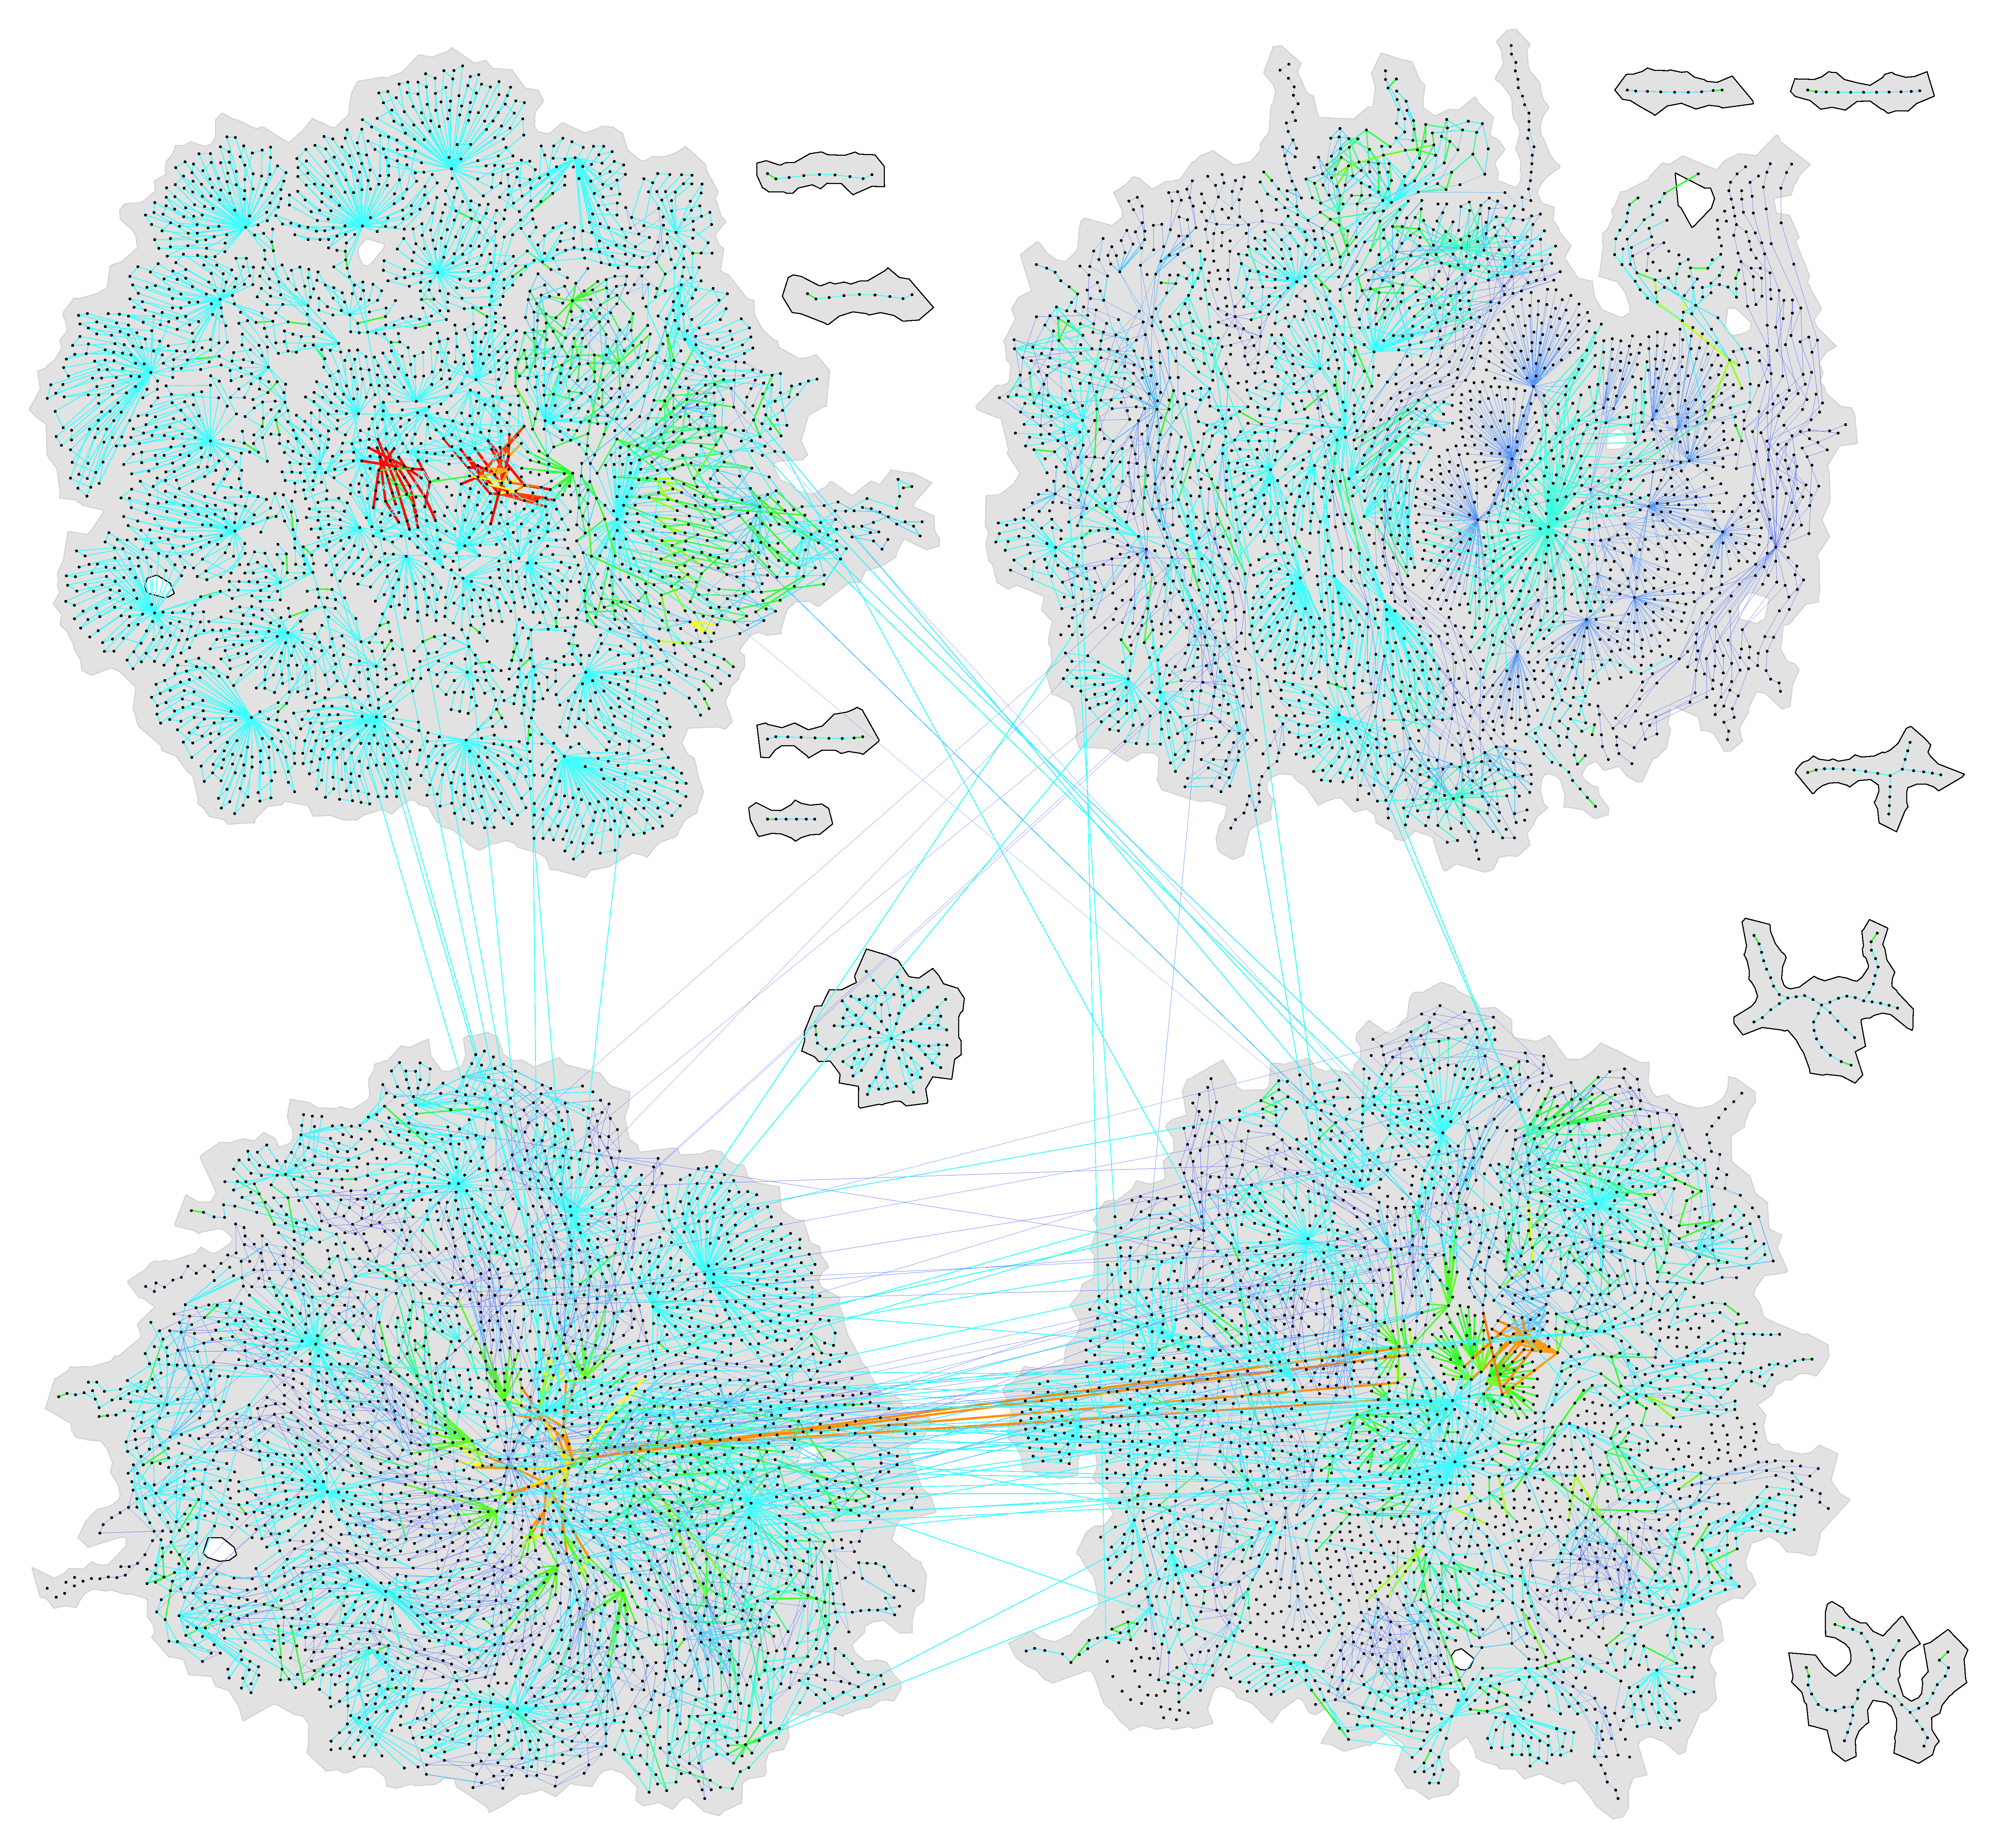
\includegraphics[width=\textwidth,height=0.9\textheight,keepaspectratio]{figs/s38584_4part}
\caption{Heatmap of messages sent during the ISCAS'89 s38584 simulation, partitioned into four partitions using the profile guided algorithm.}
\end{figure}

\begin{figure}
\centering
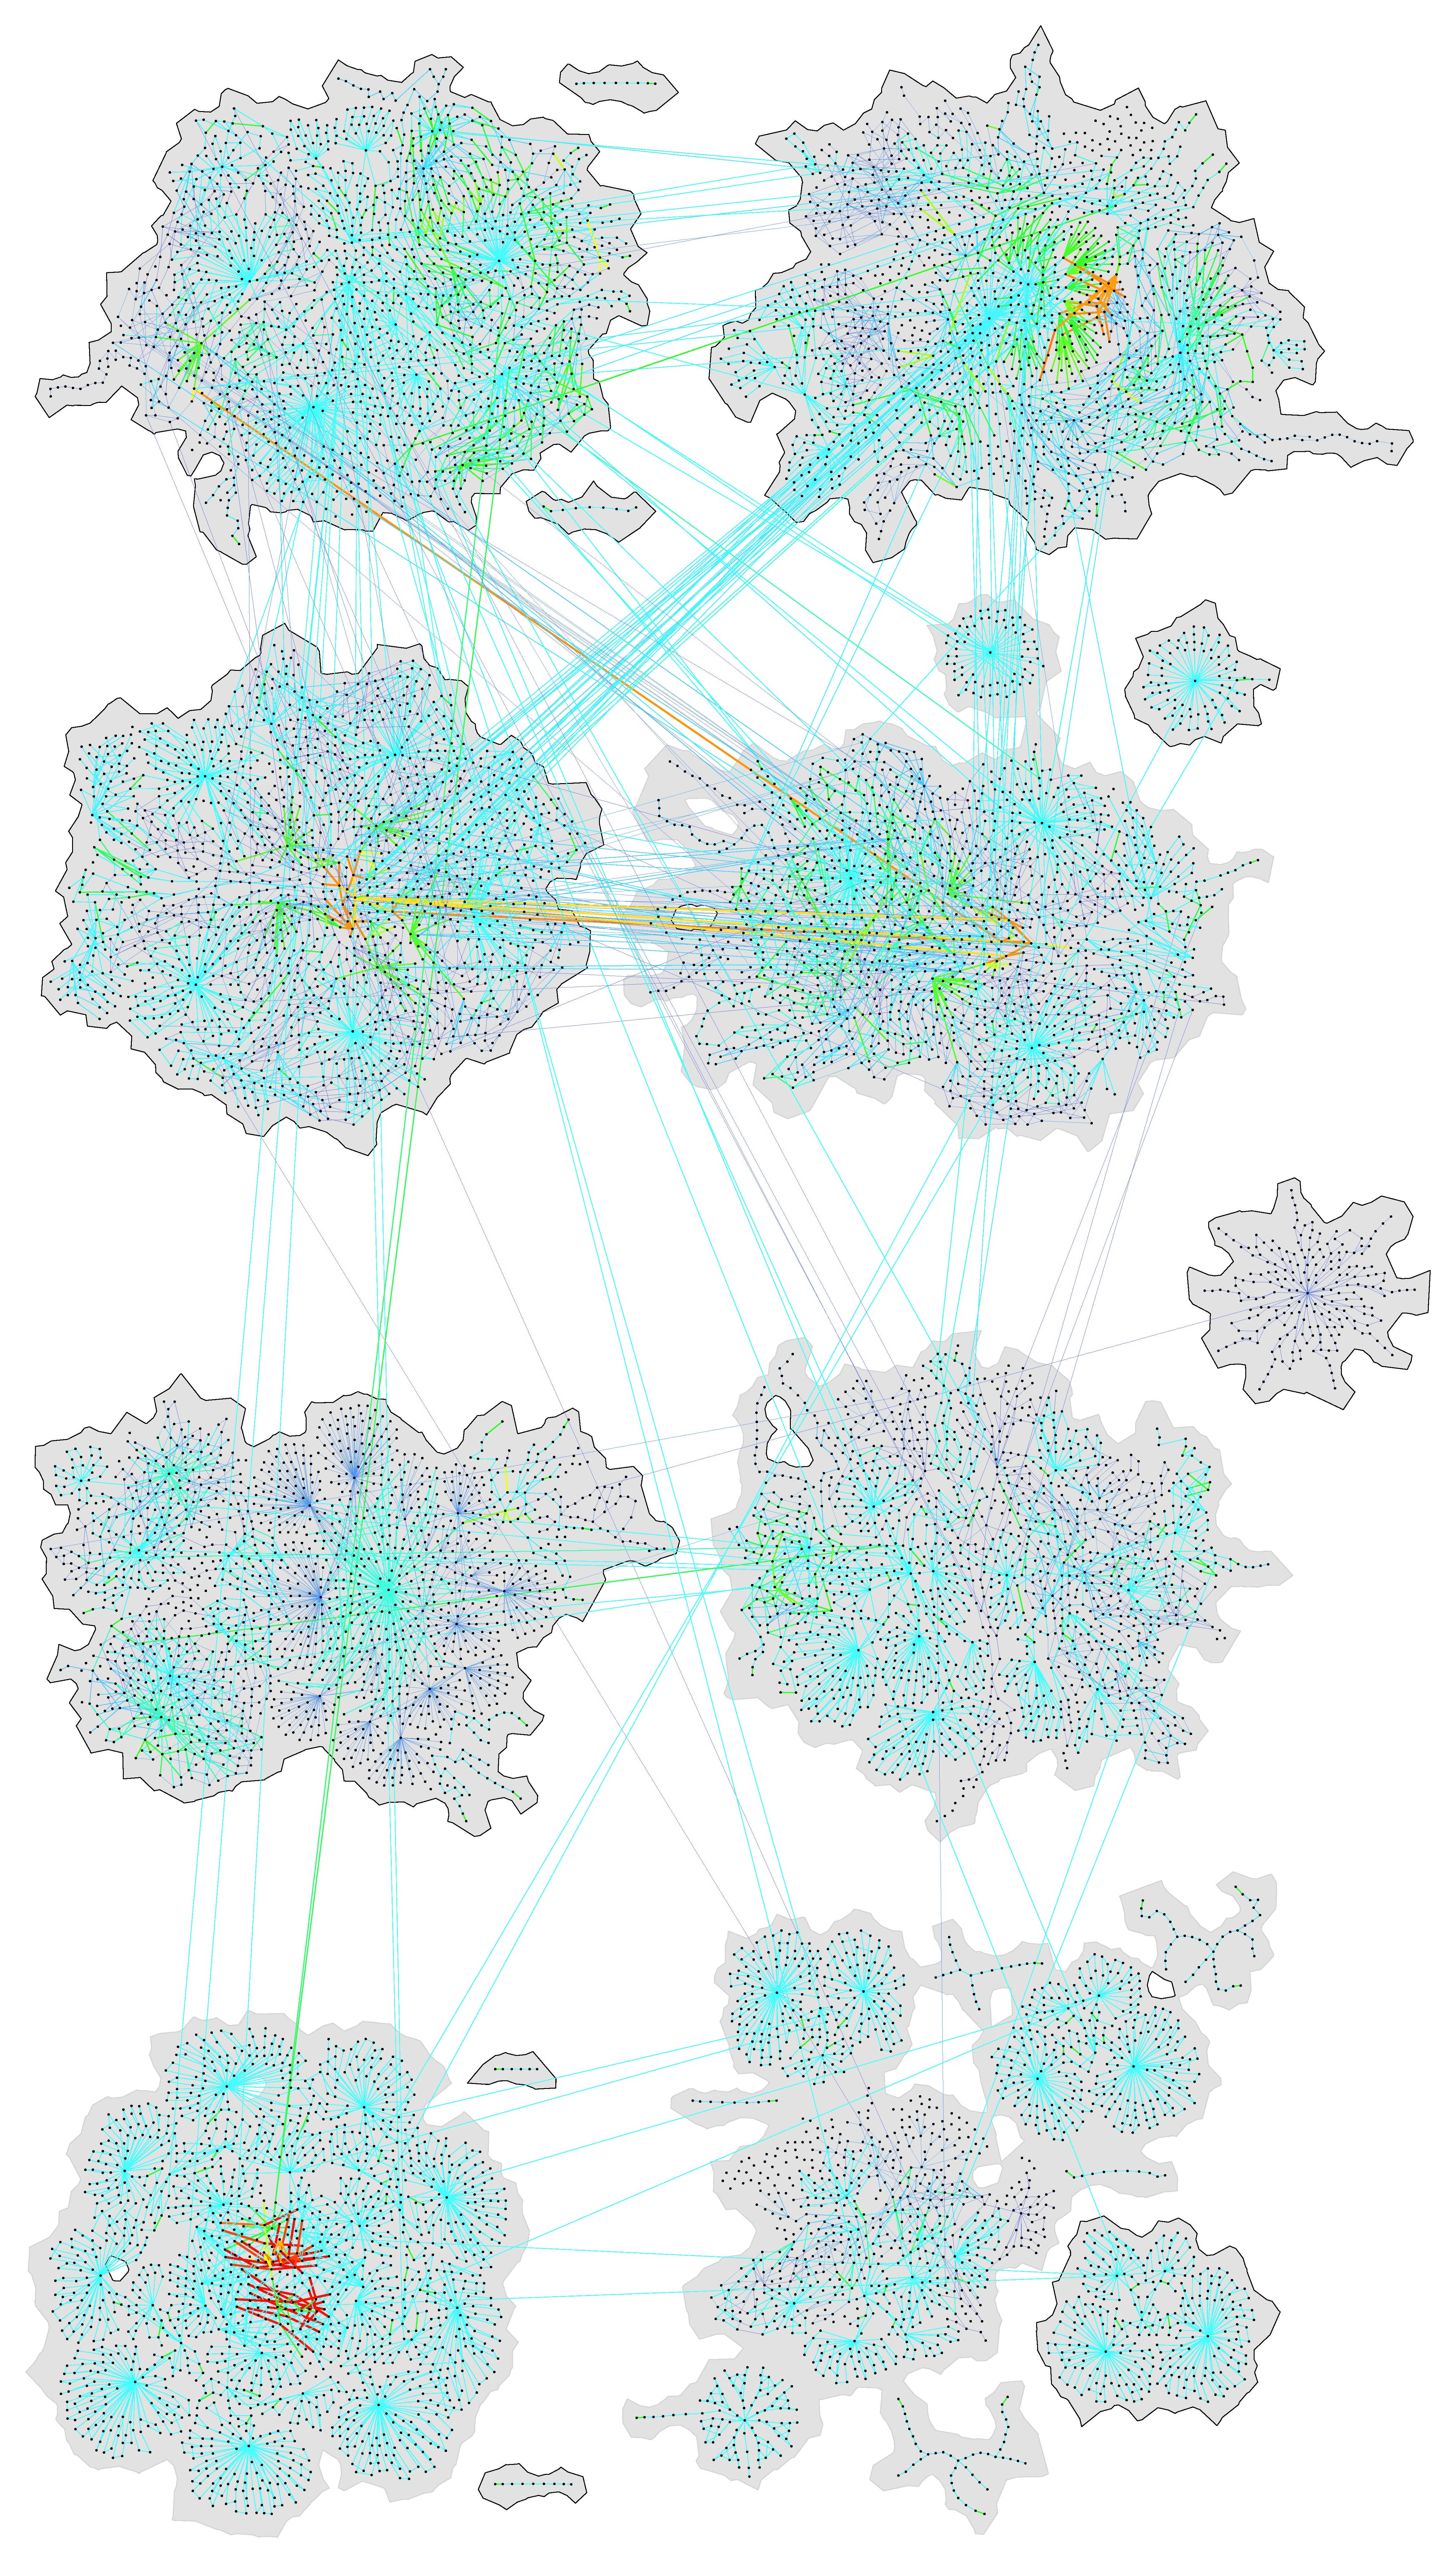
\includegraphics[width=\textwidth,height=0.9\textheight,keepaspectratio]{figs/s38584_8part}
\caption{Heatmap of messages sent during the ISCAS'89 s38584 simulation, partitioned into eight partitions using the profile guided algorithm.}
\end{figure}

\end{document}
